%\documentclass[11pt]{article}
\documentclass{article}
 
%encoding
%--------------------------------------
\usepackage[utf8]{inputenc}
\usepackage[T1]{fontenc}
%--------------------------------------
 
%Portuguese-specific commands
%--------------------------------------
\usepackage[portuguese]{babel}
%\usepackage[english]{babel}
%--------------------------------------
 
%Hyphenation rules
%--------------------------------------
\usepackage{hyphenat}
\hyphenation{mate-mática recu-perar}

%--------------------------------------
%\usepackage[top=2cm, bottom=2cm, left=2cm, right=2cm]{geometry}
\usepackage[table]{xcolor}% http://ctan.org/pkg/xcolor

\usepackage{fullpage}
%\usepackage[color]{vdmlisting}
\usepackage[hidelinks]{hyperref} 
\usepackage{longtable}
\usepackage{indentfirst}
\usepackage{graphics}
\usepackage{graphicx}
\usepackage{float}
\usepackage{enumitem}
\usepackage{wrapfig}
\usepackage{listings}
%\usepackage{natbib}
\usepackage{multirow}
\usepackage[table]{xcolor}
\usepackage{rotating}
\usepackage{placeins}
\usepackage{csquotes}
\usepackage{framed}

\usepackage{textcomp}
\usepackage{amsmath}
\DeclareRobustCommand{\perthousand}{%
  \ifmmode
    \text{\textperthousand}%
  \else
    \textperthousand
  \fi}

\hypersetup{colorlinks=true,linkcolor=blue,urlcolor=blue}

\usepackage{caption}
\captionsetup[table]{name=Tabela}

\usepackage{listings}
\lstset{language=C++, 
	numbers=none,
	firstnumber=1,
	numberfirstline=false,
    basicstyle=\linespread{0.8}\ttfamily,
    keywordstyle=\color{blue}\ttfamily,
	showstringspaces=false,
    stringstyle=\color{red}\ttfamily,
    commentstyle=\color{green}\ttfamily,
	identifierstyle=\color{darkgray}\ttfamily,
    morecomment=[l][\color{magenta}]{\#},
	tabsize=4,
    breaklines=true
}

\usepackage[
backend=biber,
sorting=ynt
]{biblatex}
\addbibresource{refs.bib}

\usepackage[margin=0.8in]{geometry}

\usepackage[toc,page]{appendix}

\newlist{legal}{enumerate}{10}
\setlist[legal]{label*=\arabic*.}

\newcommand\Tstrut{\rule{0pt}{2.6ex}}       % "top" strut
\newcommand\Bstrut{\rule[-0.9ex]{0pt}{0pt}} % "bottom" strut
\newcommand{\TBstrut}{\Tstrut\Bstrut} % top&bottom struts
\newcommand{\spheading}[2][10em]{% \spheading[<width>]{<stuff>}
  \rotatebox{90}{\parbox{#1}{\raggedright #2}}}

\begin{document}

\setlength{\voffset}{0.6in}
\addtolength{\topmargin}{-.3in}
\setlength{\textwidth}{17cm}
\setlength{\textheight}{23cm}
\setlength{\parskip}{0.5em}

\title{
\Huge\textbf{Pentago}\linebreak\linebreak
\Large\textbf{Relatório Final}\linebreak\linebreak\linebreak

\includegraphics[height=6cm, width=7cm]{feup.pdf}\linebreak\linebreak
\Large{Mestrado Integrado em Engenharia Informática e Computação} \linebreak \linebreak
\Large{Inteligência Artificial}\linebreak\linebreak
}

\author{\textbf{Grupo}\\ 
Ângela Filipa Pereira Cardoso - 200204375 - angela.cardoso@fe.up.pt \\
Bruno Miguel Dias Madeira - 201306619 - up201306619@fe.up.pt \\
Franscisco José Lopes Veiga- 201201604 - ei12170@fe.up.pt \\\linebreak\linebreak \\ \\ 
 \\ Faculdade de Engenharia da Universidade do Porto \\ Rua Roberto Frias, s\/n, 4200-465 Porto, Portugal  \linebreak\linebreak\linebreak\linebreak
\linebreak\linebreak\vspace{1cm}}
%\date
\maketitle
\thispagestyle{empty}
 
%************************************************************************************************
%************************************************************************************************

\newpage

\tableofcontents

%************************************************************************************************
%************************************************************************************************

%*************************************************************************************************
%************************************************************************************************

\newpage

%---------------------------------------------------------------------%
%---------------------------------------------------------------------%
\section{Objetivo}
 
\subsection{O Jogo Pentago}

O Pentago é um jogo de estratégia para dois jogadores, jogado num tabuleiro $6 \times 6$ dividido em 4 quadrantes $3 \times 3$, que podem ser rodados. Além do tabuleiro, o jogo é composto por 18 peças brancas, que serão usadas por um dos jogadores, e 18 peças pretas, que serão usadas pelo outro.

\begin{table}[H]
\centering
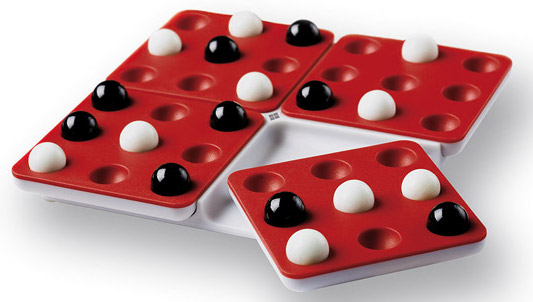
\includegraphics[height=4cm]{images/pentago-board.jpg}
\end{table}

Alternadamente, os jogadores colocam uma peça da sua cor numa casa vazia, e depois rodam um dos quadrantes 90 graus num sentido à escolha. Um jogador ganha o jogo se conseguir colocar 5 peças em linha contínua na horizontal, diagonal ou vertical, antes ou depois da rotação. Há ainda duas situações em que o jogo pode terminar em empate: se após uma rotação ambos os jogadores fizerem 5 em linha simultaneamente; ou se todas as 36 peças forem colocadas no tabuleiro e a última rotação for feita, sem que nenhum jogador obtenha 5 em linha.

Por se tratar de um jogo com regras muito simples, rapidamente se aprende a jogar. No entanto, o facto de se poderem rodar os quadrantes, faz com que por vezes seja difícil ver o objetivo do adversário, e até jogadores mais experientes podem ser derrotados por distrações. Neste sentido, é um jogo interessante, porque não é fácil de dominar.

\subsection{Uma Implementação do Pentago com Inteligência Artificial}

O nosso objetivo neste trabalho foi realizar uma aplicação para jogar Pentago no computador, com especial enfoque na criação de adversários com inteligência artificial. A aplicação permite realizar jogos em três modos distintos: humano vs humano, humano vs computador e computador vs computador. Este último modo, apesar de não ser muito comum em aplicações do mesmo tipo, é bastante útil, porque permite determinar qual a melhor entre duas implementações diferentes do jogador computador.

Dado que o ganho de um jogador corresponde exatamente à perda do outro, o Pentago é um jogo de soma zero. Neste tipo de jogos, o algoritmo minmax e as suas variantes são particularmente adequados, dado que procuram minimizar as perdas e maximizar os ganhos. Para implementar estes algoritmos, é necessário criar heurísticas que dado um tabuleiro avaliem o seu valor do ponto de vista de um dos jogadores. Neste relatório descrevemos as nossas implementações dos algoritmos minmax e as heurísticas que criamos para os jogadores computador. 

%---------------------------------------------------------------------%
%---------------------------------------------------------------------%
\newpage
\section{Especificação}

%!TEX root=main.tex

\subsection{Representação do tabuleiro}

\subsubsection{Array Unidimensional (usada no projeto principal)}

Na representação que decidimos usar um tabuleiro de Pentago é um array unidimensional indexado dado por:
\begin{equation*}
3Qx+18Qy+Px+6Py	\qquad\qquad Qx,Qy\in{0,1} \land x,y\in{0,2}.
\end{equation*}
Onde Qx e Qy indicam qual o quadrante e x e y a posição dentro do quadrante. A figura seguinte ilustra melhor como são mapeados os indexes do array no tabuleiro:

\begin{table}[H]
\centering
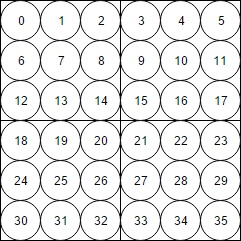
\includegraphics[height=4cm]{images/boardindexes.jpg}
\end{table}

Na prática, no código desenvolvido, não usamos $Qx$ e $Qy$ mas apenas uma única variável para escolher um quadrante quando necessitamos de realizar operações no tabuleiro. A lógica subjacente continua a mesma, apenas mais ofuscada, fazendo a indexação de quadrantes analogamente à leitura de texto (da esquerda para direita e de cima para baixo).

Além do array, na implementação, incluímos também o turno, isto é o próximo a jogar, e o estado da jogada, isto é, colocar peça ou rodar quadrante.

\subsubsection{72 bits - versão ``Pandora''}

Uma das formas de representação do tabuleiro considerada foi como uma estrutura de 72 bits (9 bytes) que podem ser usados, na linguagem de programação usada, com apenas duas variáveis: uma do tipo \verb|long| e outra do tipo \verb|char|. 

Para cada posição do tabuleiro são utilizados 2 bits, sendo que apenas 3 das 4 possíveis configurações de bits seriam usadas. Como o tabuleiro tem 36 posições, ao todo são necessários $2 * 36 = 72$ bits.

Apesar de não ser usada no projeto principal, esta representação foi implementada em \emph{PentagoPandora.cs}~(\ref{PandoraDescricao}).

\subsubsection{55 bits - apenas teorizado}

Removendo simetrias, o número de estados que um jogo de Pentago pode ter é 3.009.081.623.421.558. Isto significa que o número de estados pode ser representado em 52bits, mais alguns extra para representar as simetrias. Se houver um algoritmo que permita inferir os tabuleiros fazendo uso da gama de números de 0 ao valor acima, é possível representar um tabuleiro numa única variável que poderia ser útil para poupar recursos de memória. Tal hipótese levou a algum investimento na consideração das diferentes representações possíveis do tabuleiro.

Uma das forma de representação que conseguimos teorizar necessitaria de apenas 55 bits para representar o tabuleiro, sendo que qualquer estado possível seria identificado por um número único. Ela consiste em considerar todas as possíveis combinações de peças do tabuleiro, sendo que a busca do estado seria feita por ``camadas", inferindo em cada camada informação sobre o tabuleiro que seria usada também nas camadas seguintes. Esta forma teria um número reduzido de estados impossíveis, que representam estados de tabuleiro aparentemente corretos mas que nunca poderiam ser atingidos devido às condições de fim de jogo, sendo por isso bastante compacta. Apesar de poupar memória e ser possível descobrir se 2 estados de tabuleiro são iguais rapidamente, saber qual o tabuleiro que um número representa seria pouco eficiente pelo que a ideia foi descartada do ponto de vista de implementação. Apresentamos contudo uma representação de como se poderia inferir o estado do tabuleiro a partir de um número na gama de 55 bits e qual a fórmula usada no cálculo do número de estados.

\begin{table}[H]
\centering
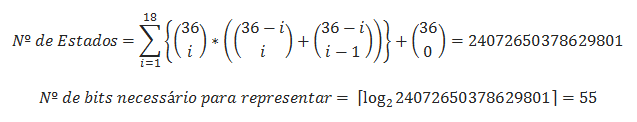
\includegraphics[width=12cm]{images/pentago_rep0.png}

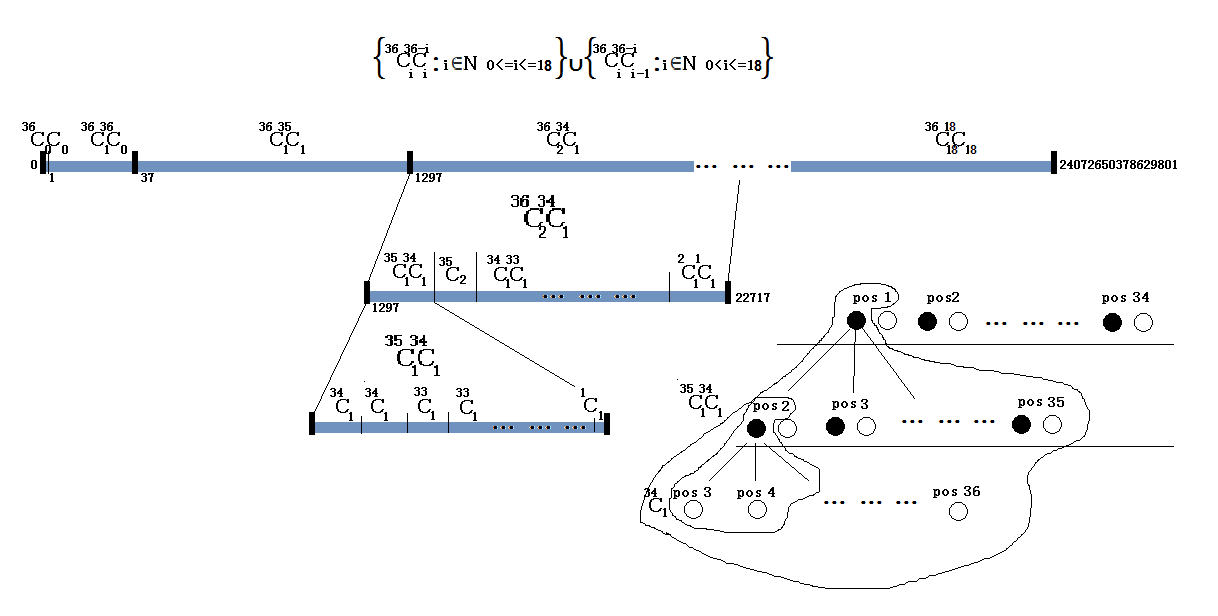
\includegraphics[height=9cm]{images/complex.png}
\end{table}

%!TEX root=main.tex

\subsection{Algoritmos}

\subsubsection{Minmax}

Quando o jogador computador tem que efetuar uma jogada, o algoritmo Minmax determina quais as jogadas possíveis. Cada uma destas jogadas é analisada da seguinte forma:
\begin{itemize}
	\item se tiver sido atingido o nível de profundidade especificado para o algoritmo, é calculado um valor para o tabuleiro, usando uma heurística do ponto de vista do computador;
	\item se a jogada conduzir ao final do jogo, é atribuído um valor ao tabuleiro tendo em conta quem ganhou, isto é, um valor positivo muito alto se ganha o computador ou um valor negativo muito baixo se ganha o adversário. Estes valores, assim como o valor atribuído em caso de empate, podem ser definidos por quem utilize a nossa implementação do Minimax e podem não ser constantes. No caso do Pentado implementado, fazemos uso do valor da profundidade para distinguir entre derrotas e vitórias que ocorrem em diferentes profundidades;
	\item se nenhuma das condições anteriores se verificar, são calculadas todas as jogadas seguintes possíveis e o processo repete-se.
\end{itemize}
Para determinar o valor da jogada original (a decisão que o computador tem que tomar no momento), entra a parte do Minmax propriamente dita:
\begin{itemize}
	\item se for a vez do adversário, o valor do tabuleiro é o mínimo dos valores das possíveis jogadas seguintes;
	\item se for a vez do computador, o valor do tabuleiro é o máximo dos valores das possíveis jogadas seguintes.
\end{itemize}

A ideia é bastante simples, dado que assumimos que o adversário fará o melhor para ele, ou seja o pior para o computador e, portanto, escolherá a jogada com um valor mínimo do ponto de vista do computador. Por outro lado, o computador a cada passo escolhe a jogada com um valor máximo para si, o que também faz todo o sentido.

\subsubsection{Minmax Alfa-Beta}

Para melhorar a eficiência do algoritmo Minmax, em termos temporais, utilizam-se cortes Alfa-Beta, que cortam ramos da árvore de decisão cuja análise é desnecessária. Em cada nó da árvore, calculam-se valores $\alpha$ e $\beta$:
\begin{itemize}
	\item $\alpha$ é o melhor valor já encontrado para o maximizador desde esse nó até à raiz;
	\item $\beta$ é o melhor valor já encontrado para o minimizador desde esse nó até à raiz.
\end{itemize}
Nos nós maximizadores atualiza-se $\alpha$ se um dos seus nós filhos apresenta maior valor que o $\alpha$ atual. Nos nós minimizadores atualiza-se $\beta$ se um dos seus nós filhos apresenta menor valor que o $\beta$ atual. Sempre que $\alpha \geq \beta$ efetuamos uma poda, isto é, não continuamos com a análise desses ramos da árvore, porque já sabemos que não apresentarão resultados que nos interessem. 

\subsubsection{Minmax Alfa-Beta Delimitado}

Este é um algoritmo consiste a adição de uma modificação ao algoritmo original de Alfa-Beta. Nele é possível definir um limite máximo e mínimo. Quando um nodo do tipo Max encontra um valor superior ao limite máximo ou um nodo do tipo  encontra um valor inferior ao limite mínimo considera-se que se encontrou uma solução suficientemente boa, não se visitando possíveis jogadas ainda visitadas num determinado nodo.

Com esta abordagem podemos facilmente cortar nós após um nodo encontrar uma jogada vencedora pois o valor de utilidade atribuído a estes tabuleiros é muito superior ao obtido, geralmente, pelas heurísticas. Além disso também é possível usar um Minmax mais flexível, que tenha mais consideração pela performance temporal em detrimento da precisão do resultado obtido.

\subsection{Funcionalidades e Otimizações}

\subsubsection{Generalização para múltiplas jogadas}

Os algoritmos implementados permitem a realização de vários movimentos (sub-jogadas) por um jogador, o que é um detalhe crítico no Pentago cuja vitória pode ser alcançada após o colocar de uma peça sem se realizar a rotação dos quadrantes. Detalhes da implementação são mencionados na secção~\ref{subjogadas_estrutura} deste relatório.

\subsubsection{Remoção de duplicados}

A fim de tentar melhorar a performance temporal são identificados e descartados tabuleiros iguais quando são efetuadas rotações de quadrantes dentro do Minmax. 

Esta verificação compara todas as posições dos tabuleiros. Provavelmente não constitui a solução mais eficaz. Nesse sentido a representação de 72 bits parece mais tentadora. Claro que  também teria algum processamento adicional devido na realização de rotações. Uma vez que não foi usada não podemos tirar conclusões sobre esta alternativa. 

Dos testes de eficiência temporal usados esta modificação apenas é benéfica em tabuleiros com poucas peças, perdendo a sua eficiência quando usada com tabuleiros com mais de 7 peças aproximadamente. A partir de 7 peças, para a maioria dos tabuleiros, a eficiência temporal com remoção de duplicados é pior do que aquela sem remoção de duplicados. No entanto, mesmo nestes casos, a perda de eficiência provocada não é substancial, pelo menos para as profundidades usadas no projeto.

\subsubsection{Simetrias}

O Pentago é um jogo particularmente interessante do ponto de vista das simetrias. O grupo de simetrias do Pentago é o grupo diedral $D_4$, que tem 8 elementos:
\begin{itemize}
	\item o elemento neutro ou identidade;
	\item 3 rotações, de 90, 180 e 270 graus centígrados;
	\item 4 reflexões, horizontal, vertical e duas diagonais.
\end{itemize}

Além destas simetrias, por vezes é ainda útil considerar simetrias de cada quadrante. De facto, o grupo de simetrias de cada quadrante é também $D_4$, mas nós apenas consideramos as reflexões na diagonal principal do primeiro quadrante. 

É de notar que quando o tabuleiro é simétrico relativamente à rotação de $90^{\circ}$ também é simétrico relativamente às rotações de $180^{\circ}$ e de $270^{\circ}$. Além disso, há várias composições de transformações cujo resultado implica outras transformações. Por exemplo, se tiver simetria de reflexão vertical e simetria de reflexão horizontal, então também tem simetria de rotação de $180^{\circ}$. Isto permite evitar verificações desnecessárias de simetrias. 

O algoritmo utilizado para validar simetrias é o que se apresenta a seguir.
\begin{enumerate}
	\item O tabuleiro é simétrico relativamente à rotação de $180^{\circ}$.
		\begin{enumerate}
			\item O tabuleiro é simétrico relativamente à rotação de $90^{\circ}$.
			\begin{enumerate}
				\item O primeiro quadrante é simétrico relativamente à sua diagonal principal. Então basta explorar as próximas jogadas nos nós acima da diagonal principal do primeiro quadrante.
\begin{table}[H]
\centering
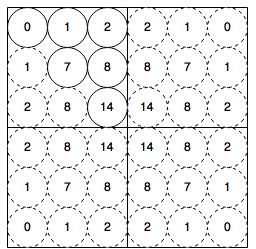
\includegraphics[height=4cm]{images/p180_90_dp0.png}
\end{table}			
				\item O primeiro quadrante não é simétrico relativamente à sua diagonal principal. Então basta explorar as próximas jogadas nos nós do primeiro quadrante.
\begin{table}[H]
\centering
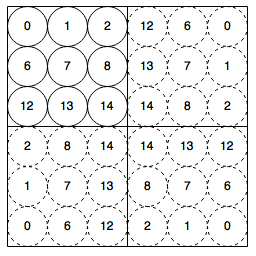
\includegraphics[height=4cm]{images/p180_90.png}
\end{table}			
			\end{enumerate}
			\item O tabuleiro não é simétrico relativamente à rotação de $90^{\circ}$, mas é simétrico relativamente à reflexão vertical.
			\begin{enumerate}
				\item O primeiro quadrante é simétrico relativamente à sua diagonal principal. Então basta explorar as próximas jogadas nos nós acima da diagonal principal do primeiro quadrante.
\begin{table}[H]
\centering
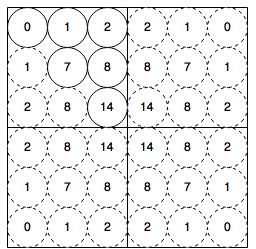
\includegraphics[height=4cm]{images/p180_rv_dp0.png}
\end{table}			
				\item O primeiro quadrante não é simétrico relativamente à sua diagonal principal. Então basta explorar as próximas jogadas nos nós do primeiro quadrante.
\begin{table}[H]
\centering
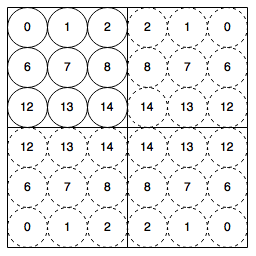
\includegraphics[height=4cm]{images/p180_rv.png}
\end{table}			
			\end{enumerate}
			\item O tabuleiro não é simétrico relativamente à rotação de $90^{\circ}$, nem é relativamente à reflexão vertical, mas é simétrico relativamente à reflexão na diagonal principal. Então basta explorar as próximas jogadas no \emph{triangulo superior}.
\begin{table}[H]
\centering
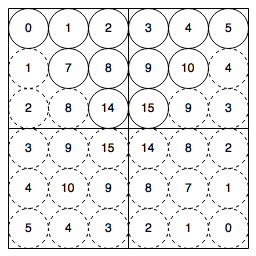
\includegraphics[height=4cm]{images/p180_dp.png}
\end{table}			
			\item O tabuleiro não é simétrico relativamente à rotação de $90^{\circ}$, nem é relativamente à reflexão vertical, nem relativamente à reflexão na diagonal principal. Então basta explorar as próximas jogadas nos nós dos dois primeiros quadrantes.
\begin{table}[H]
\centering
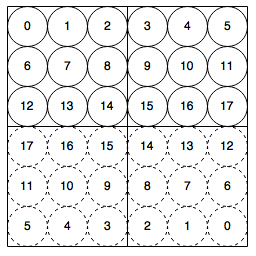
\includegraphics[height=4cm]{images/p180.png}
\end{table}			
		\end{enumerate}
	\item O tabuleiro não é simétrico relativamente à rotação de $180^{\circ}$.		
		\begin{enumerate}
			\item O tabuleiro é simétrico relativamente à reflexão vertical. Então basta explorar as próximas jogadas nos nós dos dois primeiros quadrantes.
\begin{table}[H]
\centering
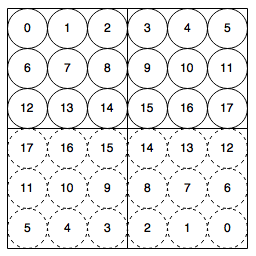
\includegraphics[height=4cm]{images/p_rv.png}
\end{table}
			\item O tabuleiro não é simétrico relativamente à reflexão vertical, mas é simétrico relativamente à reflexão horizontal. Então basta explorar as próximas jogadas no primeiro e no terceiro quadrantes.
\begin{table}[H]
\centering
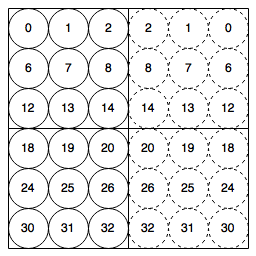
\includegraphics[height=4cm]{images/p_rh.png}
\end{table}			
			\item O tabuleiro não é simétrico relativamente à reflexão vertical, nem relativamente à reflexão horizontal, mas é simétrico relativamente à reflexão na diagonal principal. Então basta explorar as próximas jogadas acima da diagonal principal.
\begin{table}[H]
\centering
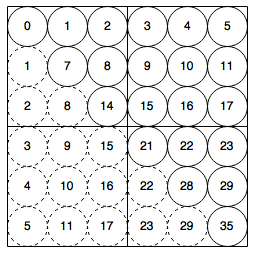
\includegraphics[height=4cm]{images/p_dp.png}
\end{table}			
			\item O tabuleiro não é simétrico relativamente à reflexão vertical, nem relativamente à reflexão horizontal, nem relativamente à reflexão na diagonal principal, mas é simétrico relativamente à reflexão na anti diagonal. Então basta explorar as próximas jogadas acima da anti diagonal.
\begin{table}[H]
\centering
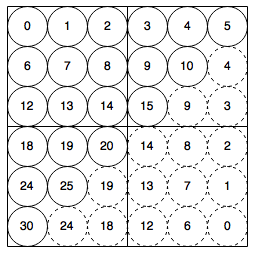
\includegraphics[height=4cm]{images/p_ad.png}
\end{table}			
		\end{enumerate}
\end{enumerate}

Uma vez que apenas podem existir simetrias quando o número de peças no tabuleiro é par, para agilizar o processamento, apenas verificamos as simetrias nesta situação. Quando o número de peças no tabuleiro é muito reduzido, a verificação de simetrias introduz melhorias significativas. Uma vez perante um número de peças maior os resultados são significativamente piores. Na versão final do projeto, foi colocada uma restrição para apenas ser efetuada validação de simetrias para tabuleiros com um número de peças reduzido. Esta restrição está em vigor nos testes de eficiência temporal apresentados.

\subsubsection{Profundidade Automática}

Ao aumentar o número de peças de um tabuleiro o número médio de nodos filho a analisar por cada nodo no Minmax diminui. Assim é possível analisar a uma profundidade mais elevada,  mantendo (aproximadamente) o mesmo tempo de execução. As profundidades usadas automaticamente face ao número de peças foram escolhidas de acordo com palpites educados, calculando o número aproximado de nós a serem visitados, sendo depois realizados ajustes manualmente após a realização de testes de eficiência temporal. Por prevenção foi dada alguma margem de erro, isto é, algumas profundidades podiam ser aplicadas com um maior número de peças no tabuleiro do que aquele que está estabelecido no código.

%!TEX root=main.tex
\newpage
\subsection{Heurísticas}

\subsubsection{Heurística 1}
%!TEX root=main.tex

A heurística 1, cujo o nome vem do facto de ter sido a primeira a ser implementada, tenta analisar as possibilidades de vitória para ambos os jogadores de uma forma relativamente ingénua. Para explicar como funciona observem-se os seguintes tabuleiros, onde os círculos a verde representam posições ocupadas pelo jogador 1, e a vermelhos as ocupadas pelo jogador 2.

\begin{table}[H]
\centering
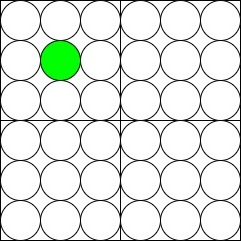
\includegraphics[height=4cm]{images/h1_block1.jpg}
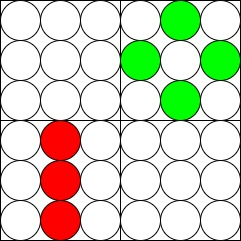
\includegraphics[height=4cm]{images/h1_block2.jpg}
\end{table}

Se atentarmos à segunda linha horizontal, em ambos os tabuleiros, podemos concluir rapidamente que o jogador 2 nunca poderá efetuar quatro em linha na segunda linha horizontal uma vez que esta se encontra bloqueada pelas peças do jogador 1. 

Podemos averiguar que temos 4 conjuntos de posições em cada um dos quadrantes que contêm a segunda linha horizontal. Quando um dos quadrantes fica com os 4 conjuntos ocupados por peças de um jogador deixa de ser possível ao jogador adversário usar essa linha para ganhar o jogo. As figuras seguintes ajudam a ilustrar esta situação no caso da segunda linha horizontal. 

\begin{table}[H]
\centering
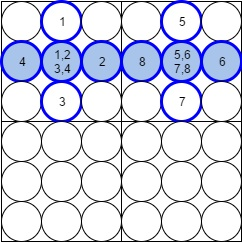
\includegraphics[height=4cm]{images/h1_pattern1.jpg}
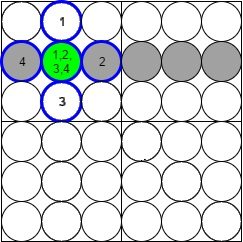
\includegraphics[height=4cm]{images/h1_block3.jpg}
\end{table}

A heurística 1 considera que o \emph{número de possibilidades} que um jogador tem para fazer 5 em linha na segunda linha horizontal é igual ao mínimo número de grupos livres (ainda não ocupados pelo adversário) entre os dois quadrantes que contêm a linha.
Este raciocínio é estendido para as outras linhas que podem ser usadas, sendo no caso das diagonais menores, considerados o mínimo de 3 quadrantes. As figuras seguintes ajudam a perceber o quais os grupos usados para cada linha em cada um dos quadrantes.

\begin{table}[H]
\centering
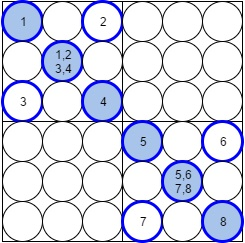
\includegraphics[height=4cm]{images/h1_pattern2.jpg}
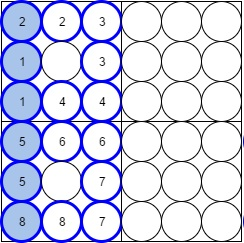
\includegraphics[height=4cm]{images/h1_pattern3.jpg}
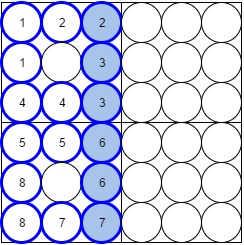
\includegraphics[height=4cm]{images/h1_pattern4.jpg}
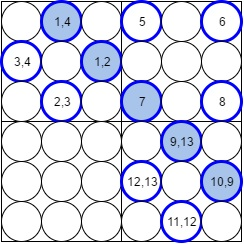
\includegraphics[height=4cm]{images/h1_pattern5.jpg}
\end{table}

A heurística inclui também uma variável \verb|bias| que permite dar mais peso às possibilidades dos jogador ou às possibilidades do jogador adversário. Assim é possível parametrizar a heurística de modo a que tenha um comportamento mais otimista, pessimista, defensivo ou ofensivo. A seguinte fórmula apresenta como é obtido um valor pela heurística, onde $Pm$ é o número de possibilidades para o próprio, $Po$ o número de possibilidades para o oponente e alfa a variável de \verb|bias|.

\begin{equation}
\alpha Pm-(1-\alpha)Po  \qquad\qquad\alpha\in[0,1] 
\end{equation}

Esta consideração é algo ingénua pois é possível que o adversário, fazendo uso das rotações, não permitir o uso de determinadas linhas enganando assim a heurística. Além disso se não é possível usar o minmax para evitar jogadas fatalistas no inicio do jogo, dado existirem demasiadas possibilidades a analisar, a heurística 1, isoladamente, não permite criar um adversário muito forte pois é muito passiva em relação ao estado do tabuleiro, não averiguando derrotas eminentes.

Foram também adicionados pesos aos diversos tipos de linhas. Assim, é possível ao algoritmo priorizar ou desprezar alguns tipos de linhas. Sem entrar em detalhe nos tipos de linhas considerados, intuitivamente estes pesos parecem ser importantes para desprezar as diagonais pequenas que não podem ser usadas em ataques de duas pontas e que ocupam 3 quadrantes. Foi realizada alguma experimentação com estes pesos mas não se chegou a uma solução ideal e não foram realizados testes similares aos apresentados nos anexos dado que já existiam demasiadas variáveis a testar. A adição destas nos testes ia aumentar o número de testes a realizar consideravelmente caso se testasse para todas as possíveis combinações dos \verb|biases|(pesos) na heurística 1 e 1.2.



\subsubsection{Heurística 1.2}
%!TEX root=main.tex

A heurística 1.2 surgiu como na tentava de melhorar a heurística 1. Esta heurística faz o que a sua predecessora já fazia e adicionalmente mais algumas avaliações semelhantes que visão evitar jogadas fatalistas ou aproveitar oportunidades ofensivas. Para tal a heurística considera além do \emph{número de possibilidades} o \emph{número de possibilidades fortes}. 
Para explicar o que o algoritmo entende como possibilidades fortes vamos atentar a segunda linha horizontal do tabuleiro do Pentago. 

\begin{table}[H]
\centering
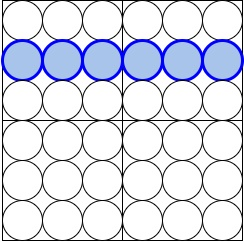
\includegraphics[height=3.5cm]{images/h12_hline.jpg}
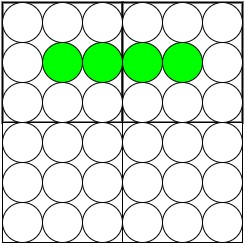
\includegraphics[height=3.5cm]{images/h12_fatal.jpg}
\end{table}

Podemos observar que o tipo de padrão usado na figura à direita é interessante do ponto de vista ofensivo, pois cria uma vitória garantida, e é contra este género de situações que o algoritmo tenta precaver-se ou tirar proveito ofensivo.
Para tal, o algoritmo contabiliza 2 tipos de casos. Denominemos esses tipos de tipo \emph{forte} e de tipo \emph{muito forte} sendo que qualquer caso que seja do tipo muito forte é também um caso do tipo forte mas o inverso pode não ser verdade. Considera-se um caso forte quando um grupo, dos definidos na heurística 1, está ocupado por peças de um jogador. Um caso muito forte acontece quando um grupo está ocupado por peças de um jogador e a sua extensão no mesmo quadrante se encontra sem uma peça adversária (podendo estar vazia ou não). Assim as 3 imagens seguintes ilustram respetivamente 2 jogadas do tipo muito forte e uma do tipo forte.

\begin{table}[H]
\centering
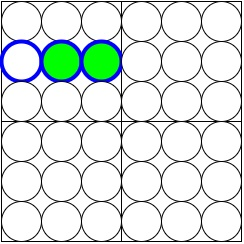
\includegraphics[height=3.5cm]{images/h12_VS.jpg}
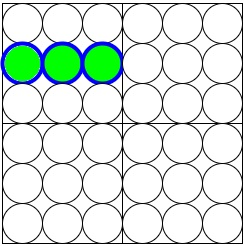
\includegraphics[height=3.5cm]{images/h12_VS2.jpg}
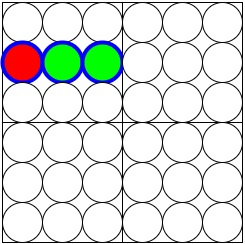
\includegraphics[height=3.5cm]{images/h12_S.jpg}
\end{table}

Depois de contabilizadas estes casos o número de jogadas fortes para a segunda linha horizontal é dada pela seguinte fórmula:
\begin{equation}
F_hor2 = max( min(F_1,M_1) , min(M_2,F_2) )
\end{equation}
Onde $Fi$ e $Mi$ representam respetivamente o número de casos fortes e o número de casos muito fortes no quadrante $i$. Os quadrantes usados, são os que contêm a linha como mostra a figura seguinte.

\begin{table}[H]
\centering
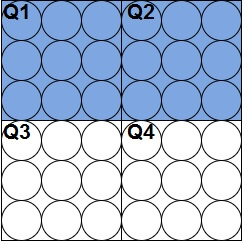
\includegraphics[height=3.5cm]{images/boardsQuadrants.jpg}
\end{table}

Assim, para melhor ilustrar a contabilização referida, são apresentadas abaixo exemplos onde o número de jogadas fortes para a segunda linha horizontal são respetivamente 1, 1, 1 e 2.

\begin{table}[H]
\centering
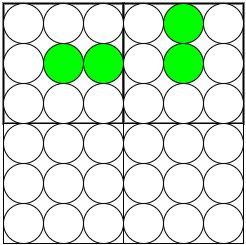
\includegraphics[height=4cm]{images/h12_ex1.jpg}
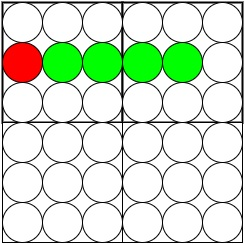
\includegraphics[height=4cm]{images/h12_ex2.jpg}
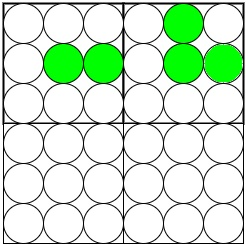
\includegraphics[height=4cm]{images/h12_ex3.jpg}
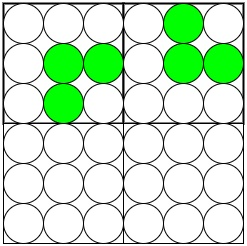
\includegraphics[height=4cm]{images/h12_ex4.jpg}
\end{table}

A mesmos cálculos são efetuados para as outras linhas (excluindo s diagonais menores que são tratadas de forma diferente) para ambos os jogadores. A heurística usa o número de jogadas fortes para o jogador (com valor positivo), para adversário (com valor negativo) e também as possibilidades da heurísticas 1. Todas estas componentes têm um peso associado que confere à heurística alguma flexibilidade podendo esta variar não só entre uma abordagem otimista ou pessimista mas também por abordagem mais passiva ou reativa.

Apesar destas considerações a heurística têm algumas dificuldades em lidar com  limitações de profundidade no Minmax pelo que foi implantada uma versão relaxada. Na sua versão relaxada consideram-se como fortes os blocos ocupados com pelo menos uma peça do jogador e nenhuma do adversário, tal como apresentado na ilustração abaixo.

\begin{table}[H]
\centering
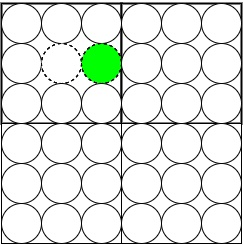
\includegraphics[height=4cm]{images/h12_relax.jpg}
\end{table}

Apesar de melhorar a sua predecessora também herda as suas fraquezas não sabendo lidar com as rotações do jogador adversário.



\subsubsection{Heurística A}
%!TEX root=main.tex

Esta heurística foi inspirada pelo guia estratégico~[2].

Há 4 formas de obter 5 em linha e ganhar um jogo de Pentago:
\begin{itemize}
	\item Monica - numa das diagonais principais do tabuleiro - força relativa 3
\begin{table}[H]
\centering
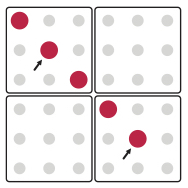
\includegraphics[height=3.7cm]{images/monica.jpg}
\end{table}
	\item Meio - na vertical ou na horizontal através do meio de dois quadrantes adjacentes - força relativa 5
\begin{table}[H]
\centering
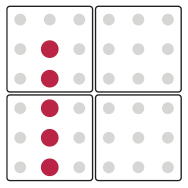
\includegraphics[height=3.7cm]{images/middle.jpg}
\end{table}
	\item Direito - na vertical ou na horizontal usando os bordos de dois quadrantes adjacentes - força relativa 7
\begin{table}[H]
\centering
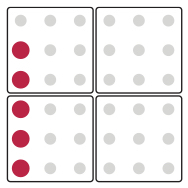
\includegraphics[height=3.7cm]{images/straight.jpg}
\end{table}
	\item Tripla - diagonalmente, abaixo ou acima das diagonais principais do tabuleiro - força relativa 9
\begin{table}[H]
\centering
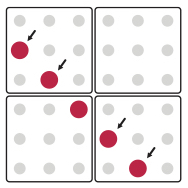
\includegraphics[height=3.7cm]{images/triple.jpg}
\end{table}
\end{itemize}

Para cada uma destas estratégias, considera-se a sua versatilidade, isto é, o número de diferentes possibilidades de aproveitar parte das peças quando um dos caminhos é bloqueado pelo adversário. Além disso, também nos interessa a dificuldade que o adversário tem de se defender contra um jogador que use a estratégia. São esses dois fatores que determinam a força relativa.

Dada uma posição do jogo, a heurística A começa por percorrer cada uma das linhas em que é possível ganhar e calcular o número de peças de cada cor. No entanto, apenas nos interessa contabilizar as peças quando há possibilidade do jogador conseguir ganhar nessa linha. Para isso, vamos verificar quantas peças há no interior da linha e quantas peças há nos bordos, dado que peças do adversário no interior bloqueiam imediatamente e para bloquear nos bordos são necessárias duas peças. Depois de efetuada esta contagem, sabemos quão forte é a posição de cada jogador em cada linha. Por exemplo, se há 3 peças brancas no interior e nenhuma peça preta em toda a linha, a posição branca é muito forte, porque basta mais uma peça para assegurar a sua vitória. 

No passo seguinte, usamos as forças relativas e as contagens para calcular o valor do tabuleiro. Sendo~$b$ o número de peças brancas,~$p$ o número de peças pretas e~$r$ a força relativa na linha em questão, adicionamos~$r^b - r^p$ ao valor previamente calculado. Este valor está a ser calculado assumindo que a IA está a jogar com as peças brancas, mas caso esteja a jogar com as pretas, basta multiplicar por -1 no final. O motivo pelo qual usamos a potência, é para garantir que ter várias peças na mesma linha é mais valorizado do que ter as mesmas peças espalhadas por linhas diferentes.

O método acima é usado para calcular o valor de todos os 8 tabuleiros que se obtém do tabuleiro atual por rotação de um quadrante. Depois disso, é usado o máximo ou o mínimo destes tabuleiros rodados, consoante o próximo jogador é a IA ou o adversário, tal como no minmax.

Em relação às forças relativas, apesar de querermos favorecer determinadas estratégias em detrimento de outras, não usamos os valores 3, 5, 7, e 9, porque devido ao uso de potências, eles conduzem a discrepâncias enormes entre jogadas, que fariam com que algumas das estratégias fossem completamente desprezadas. Sendo assim, após alguns cálculos com várias posições de jogo, optamos pelos valores 1.13, 1.15, 1.17 e 1.19. Isto contribui também para que os valores finais do tabuleiro sejam pequenos, o que será usado noutras considerações da heurística como veremos adiante. Dada a arbitrariedade da escolha dos valores, decidimos efetuar experiências estatísticas para determinar os melhores valores, mas isso será visto mais adiante na secção das experiências.

Observando jogos em que a heurística A perdia, rapidamente conseguimos determinar algumas das suas falhas. A primeira destas observações é que se um jogador conseguir 4 em linha com as duas pontas abertas (em jogadas do tipo monica, meio ou direito), então irá ganhar na próxima jogada, a não ser que o seu adversário ganhe já nesta. Assim, ao detetar estas situações a heurística A ignora todos os outros cálculos e dá valor 100 ao tabuleiro se ganha e -100 se perde.

Outra maneira certa de ganhar é conseguir duas ou mais linhas em que apenas falta uma peça para ganhar. Estas situações também foram introduzidas como exceção na heurística A, embora possam levar a alguns falsos positivos, quando ambas as linhas de vitória necessitam de uma peça na mesma posição do tabuleiro.

Finalmente, fizemos ainda algumas pequenas alterações aos valores da heurística:
\begin{itemize}
	\item se tivermos 4 peças em linha com as pontas abertas, mas for a vez do adversário, calculamos o valor como se fossem 10 peças, para que seja claramente mais valorizada que as restantes;
	\item se faltar apenas uma peça para obter 5 em linha e não estivermos na situação anterior, incrementamos a contagem de peças em 1;
	\item se houver 1, 2 ou 3 peças não bloqueadas na mesma linha (monica, meio ou direito), como ambas as pontas abertas, incrementamos a contagem em 1.
\end{itemize}

\subsubsection{Heurística A hacked}

A heurística A hacked não apresenta nenhuma construção nova face às anteriores. Na verdade apenas aparece na secção de especificação para ser referida na mesma secção das outras heurísticas neste relatório. A heurística A hacked resulta de experimentação, tendo sido descoberto, combinando pesos das diferentes heurísticas implementadas, que a heurística A tinha alguma facilidade em perder nas diagonais principais. A heurística A hacked apareceu como uma contra-heurística à A fazendo uso de funcionalidades da heurística 1.2 para evitar perder nas diagonais principais. Atualmente a heurística A star apresenta melhores resultados ao usar uma profundidade de 4 (2 jogadas).

\subsubsection{Heurística A star}

Esta heurística é uma melhoria da heurística A. A ideia básica é a mesma, mas introduzimos mais algumas verificações e alteramos outras. Além disso, nesta heurística também é possível determinar se se estudam todos os tabuleiros rodados quando a jogada é de rotação. No entanto, como veremos na secção das experiências, o desempenho da heurística é melhor quando se estudam todas as rotações.

Uma das mudanças essenciais nesta heurística é que há uma maior preocupação com quem é o próximo jogador a jogar. Por exemplo, imaginemos que ambos os jogadores têm 4 em linha com as duas pontas abertas. Então, quem irá ganhar é o próximo a jogar. Por outro lado, se apenas um dos jogadores estiver nessa posição, mesmo que não seja a vez dele, ele irá ganhar a seguir, a não ser que o outro ganhe antes por outra situação. Sendo assim, há que estudar em todos os tabuleiros rodados, quais as possibilidades de vitória dos dois jogadores. O próximo a jogar apenas precisa que um dos rodados lhe dê vitória. Enquanto que o outro precisa que um dos rodados lhe dê vitória e nenhum dê ao seu adversário.

Outra mudança significativa tem a ver com possibilidades de vitória, ainda que não seja certa. Isto é, com situações em que um dos jogadores ganha, a não ser que o outro o impeça. Nesses casos o tabuleiro é classificado com os valores 50 ou -50 consoante é o jogador computador que tem a possibilidade de ganhar ou o seu adversário. Mais uma vez, isto é estudado tendo em conta todos os rodados e quem é o próximo a jogar.

Em vários aspetos, esta heurística efetua correções à heurística A, isto é, calcula o valor da forma que realmente se pretendia fazer em A, mas que pela complexidade da heurística não foi inicialmente conseguido. No entanto, como a performance da A por vezes é melhor que a da A star, optamos por manter as duas heurísticas no jogo.

Usando profundidade 4, a profundidade máxima que se pode usar nas nossas máquinas que ainda obtém uma reposta imediata do ponto de vista do utilizador, esta é a única heurística que com os valores das forças relativas default consegue precaver-se contra uma tática ofensiva específica no Pentago. Ao controlar o centro dos quadrantes e atacar pelas diagonais as outras heurísticas perdem se não usarem profundidades mais elevadas. 

\newpage
\section{Desenvolvimento}

%!TEX root=main.tex

\subsection{Ferramentas utilizadas}

\subsubsection{Geral}

Para partilha de documentação, código e backups de segurança foi usado o \href{https://github.com/}{Github}.
O repositório está disponível em ... ... ...

Foi usado o \href{http://andrejv.github.io/wxmaxima/}{wxMáxima} para realização de cálculos diversos.

Para a elaboração de documentação e do relatório foram usados o \href{https://www.draw.io/}{Draw.io} e o \href{https://www.overleaf.com}{Overleaf}.

\subsubsection{Protótipo Inicial em Consola}

Foi usado o \href{https://eclipse.org/mars/}{Eclipse Mars} na implementação do protótipo inicial do jogo em Java. Este protótipo apenas funcionava em consola e ainda apresentava algumas inconsistência. Terá sido exportado para C\# para que se pudesse numa fase posterior integrar o projeto com o \href{https://unity3d.com/pt}{Unity3d}. 

\subsubsection{Código Core}

O código relativo ao Pentago e á inteligência artificial foram desenvolvidos na linguagem de programação C\#, no \href{https://www.visualstudio.com/}{Visual Studio} IDE para Windows OS. Como um dos elementos usou MAC OS X foi usado também o ?????????????? para trabalhar em Windows através de Máquina Virtual. Alternativamente poderia ter sido utilizado o \href{http://www.monodevelop.com/}{Monodevlop}, também compatível com MAC OS X.
A possibilidade de utilizar \emph{Partial Classes} em C\# ofereceu alguma flexibilidade adicional aos elementos do grupo ao permitir trabalhar nos mesmos módulos sem que ocorram grandes conflitos nas diferentes versões do código.

\subsubsection{Jogo com Interface Gráfica}

Para a criar o jogo Pentago com uma interface gráfica apelativa foi utilizado o \href{https://unity3d.com/pt}{Unity3d}. Todo o código, excluindo \emph{enhancements} visuais foi criado de raiz, sendo integrado com os módulos do projeto em consola desenvolvido no Visual Studio. 
Foi também usado o \href{https://www.blender.org/}{Blender}. na criação dos modelos 3d para interface gráfico do jogo.

\subsubsection{Testes de Performance temporal e de desempenho das Heurísticas}

Os dados que apresentamos neste relatório demoraram um tempo considerável a ser recolhidos, desde um dia no caso dos testes para avaliar o desempenho das heurísticas, a aproximadamente 3 no caso dos testes de performance temporal. Assim, para a realização destes, foram usados dois desktops controlados remotamente. Para a maioria dos testes foi utilizado um desktop com os seguintes características:
\begin{itemize}
\item Windows 10 SO, 64 bits
\item Processador Pentium(R) Dual-Core CPU E5500 @ 2.8GHz 2.8GHz 
\item Ram instalada 4GB(3.65GB utilizável)
\end{itemize}
Apenas nos testes de performance temporal com 100 tabuleiros foi usado um desktop com as seguintes características: 
\begin{itemize}
\item Windows 8 SO, 64 bits
\item Processador Pentium(R) Dual-Core CPU E5700 @ 3GHz 3GHz 
\item Ram instalada 2GB
\end{itemize}




%!TEX root=main.tex
\subsection{Minmax Genérico}

Para que o Minmax pudesse ser reutilizado em outros jogos foi implementada a classe Genérica MinMax e o Interface IGameRules, O IGameRules estabelece um conjunto de métodos que devem ser implementados de modo a que se possa correr o Minmax sobre um jogo especifico.%Alternativamente, todos os métodos estabelecidos no IGameRules poderiam ser \emph{delegates} (estrutura semelhante a apontadores de funções) na classe MinMax. Esta segunda solução tornaria o Minmax ligeiramente mais flexível na implementação de hacks e permitiria poupar a implementação de uma classe caso os métodos já estivessem todos implementados por quem quisesse fazer uso deste. Por questões de organização de código não resolvemos optar por esta alternativa.
Estes fazem uso de duas estruturas de dados uma para representação do estado do jogo e outra para representação de jogadas que devem ser fornecidas por quem quiser fazer uso deste Minmax genérico. 
\label{subjogadas_estrutura}
De modo a permitir as sub-jogadas presentes no Pentago e também qualquer conjunto de sub-jogadas possível em outros jogos, em vez de alternarmos entre nodos \emph{Min} e \emph{Max}. obrigamos, através da Interface IGameRules, a implementação de um método que diz qual o nodo a seguir consoante o estado do tabuleiro. Isto obrigado que as representação do estado de jogo permitam identificar o tipo nodo, seja de forma direta ou indireta. No caso da nossa implementação do Pentago esta identificação é direta, guardando de quem é o turno na estrutura que representa o tabuleiro. Alternativamente, poderia ser indireta contando o número de peças de cada jogador no tabuleiro, o que não foi usado devido ao óbvio decréscimo na eficiência temporal do Minmax. Em consequência desta decisão de implementação seria necessário, em muitos jogos, ter sempre o turno na estrutura que representa o estado de jogo pois o tabuleiro só por si pode não ser suficiente para identificar o tipo de nodo.

As primeiras iteraç\~oes relativas à primeira jogada são efetuadas de forma relativamente diferente do resto do algoritmo, guardando o conjunto de sub-jogadas que o jogador faz até terminar a sua jogada. Esta modificação foi implementada a pensar na componente de Interdace Gráfica do jogo.
Alternativamente ao caminho seguido, seria também possível usar o Minmax apenas usando estados do jogo. Nesta alternativa, de modo a representar uma jogada na Interface Gráfica seria necessário ter uma função que obtivesse uma jogada (ou várias) analisando o tabuleiro inicial e final. 

\subsection{Estrutura do código}

\subsubsection{Diagrama de Classes}

\begin{table}[H]
\centering
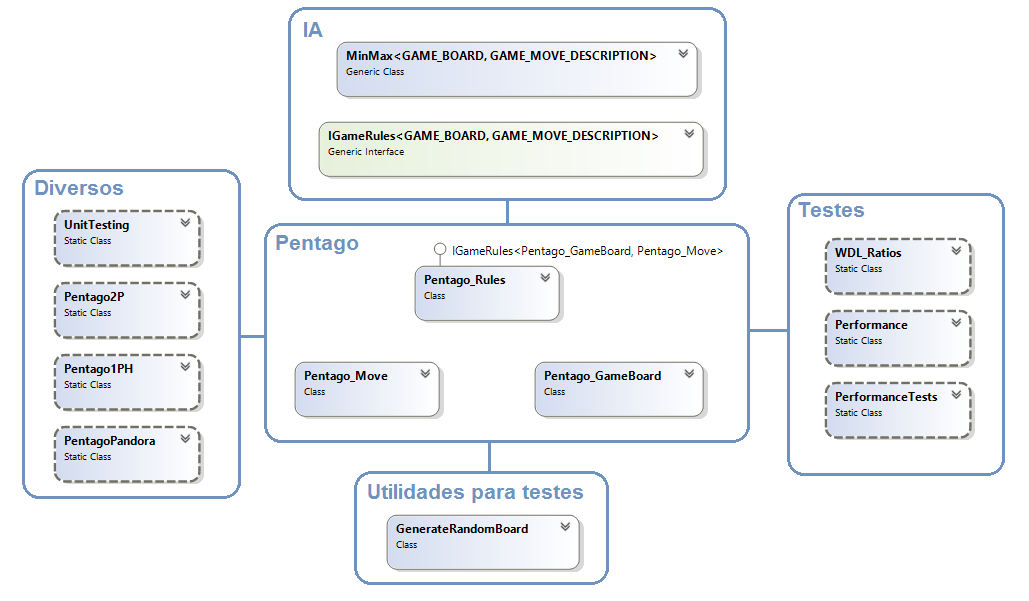
\includegraphics[height=8cm]{images/ClassDiagram1.png}
\end{table}

\subsubsection{Descrição das Classes e Interfaces}

\begin{itemize}  

\item MinMax \\
Contem a implementação genérica do algoritmo de Minmax e variantes.

\item IGameRules \\
Interface necessária à implementação de um Minmax genérico, não dependente do jogo que analisa. Uma implementação da interface deve conter duas estruturas de dados diferentes, uma para representação do ambiente de jogo (tabuleiro no caso do Pentago) e outra para representação das jogadas a efetuar sobre este. A Interface pode ser consultada no anexo ~\ref{IGameRules}.

\item Pentago\_GameBoard \\
Contem o array que representa o tabuleiro. Contem também uma variável que indica o qual o jogador a jogar e ainda qual o estado da jogada (colocar peça ou rodar quadrante). Também contem métodos auxiliares para identificar fim de jogo, clonar tabuleiros, transformar índices do tabuleiro e coordenadas e virse-versa. A classe é necessária para fazer uso da interface implementada.

\item Pentago\_Move \\
Contem informação necessária para representar uma jogada. Havendo dois tipos de jogadas poderia alternativamente optar-se pela a criação de 2 subclasses, uma para cada tipo de jogada ao invés de guardar as duas numa mesma. A classe é necessária para fazer uso da interface implementada.

\item Pentago\_Rules \\
Classe que implementa a Interface IGameRules para o Pentago. Contem também as funções de heurística, métodos para identificação de simetrias e de tabuleiros idênticos. A classe é extensa e foi divida em vários ficheiros. Em conjunto com Pentago\_Move e Pentago\_GameBoard formam a implementação do jogo concreto.

\item GenerateRandomBoard \\
Como o nome sugere a classe é responsável pela geração de tabuleiros aleatórios que são usados nos testes de \verb|performance|. 

\item WDL\_Ratios \\
Responsável por testar a \verb|performance| das heurísticas e do Minmax em termos de taxa de vitórias, derrotas e empates e fazer output dos resultados já formatados para serem inseridos em Latex.

\item Performance \\
Classe que testa a \verb|performance| temporal de uma heurística para um dado conjunto de tabuleiros.

\item PerformanceTests \\
Classe responsável por testar a \verb|performance| temporal das várias heurísticas. 

\item PentagoPandora \\
\label{PandoraDescricao}
Classe cuja única função é descobrir e exportar para memória não volátil uma árvore de Minmax apenas para o primeiro jogador, com raiz no tabuleiro inicial, que permita garantir a vitória. Não tendo sido totalmente otimizada para efetuar o seu objetivo, acabou por ser deixada de lado uma vez que saia do âmbito do projeto.

\item Pentago2P \\
Classe que apenas implementa uma versão do Pentago para 2 jogadores em consola. Usada inicialmente para testar o código.

\item Pentago1PH \\
Apenas usada no inicio do desenvolvimento, antes de codificado o algoritmo de Minmax. Permitia a um jogador humano jogar contra um minmax com profundidade de 1 jogada.

\item UnitTesting \\
Classe com testes unitários. 

\end{itemize}

\subsection{Outros Detalhes}

\newpage
%!TEX root=main.tex

\section{Experiências}

Foram realizados 2 tipos de experiências distintas. As primeiras experiências foram desenhadas para testar a qualidade das heurísticas implementadas. Isto é, para determinar se os jogadores computador que usam estas heurísticas conseguem atingir bons desempenhos a jogar Pentago. Nomeadamente, tendo duas heurísticas diferentes a jogar Pentago, interessa-nos saber qual ganha. O segundo grupo de experiências pretende determinar qual a eficiência dos algoritmos implementados. Em particular, queremos comparar estes algoritmos entre si.

\subsection{Qualidade das Heurísticas}

As estatísticas apresentadas nesta secção referem-se ao jogador destacado a negrito. Por exemplo, o número de vitórias refere-se a vitórias desse jogador. As vitórias, derrotas, empates e número médio de turnos são representados respetivamente pelas cores azul, vermelha, verde e preta. As três primeiras são apresentadas em permilagem. Todos valores originais foram arredondados para baixo pelo que o somatório das componentes pode n\~ao igualar 1000\perthousand. 

O jogador artificial que jogar com as brancas inicia a partida (ao contrário do Pentago original). 

As informações apresentadas abaixo do nome das heurísticas referem-se aos pesos/opç\~oes usadas. Nas heurísticas 1 e 1.2 são sempre usados (e ocultados nas tabelas) os pesos \verb|default| usados para os diferentes tipos de linhas. Isto porque consideramos que a sua inclusão nos testes não se justifica, dada a reduzida relevância para projeto. Muitas das combinações usadas foram descobertas ao testar, de forma automatizada, as heurísticas com valores pseudo-aleatórios (dentro de determinados intervalos).

Para cada cada heurística os dados apresentados referem-se a:
\begin{itemize}  
	\item 1 - \verb|bias|
	\item 1.2 Relaxada? (Y=sim, N=não); Usa Hack Diagonal? (Y=sim, N=não); possibilidades ; possibilidades para oponente; possibilidades fortes; possibilidades fortes para oponente
	\item A - monica ; meio ; direito ; tripla
	\item A hacked - Pesos da 1.2 ; Pesos da A
	\item A star - Pesos da A ;  Analisa Rotaç\~oes? (Y=sim,N=não)
\end{itemize} 

A primeira ocorrência de uma heurística numa tabela apresenta sempre os pesos \verb|default| da mesma.

Além de testes automáticos foram realizadas também alguns jogos de humano contra as heurísticas implementadas. Para uma profundidade de 4 a heurística A e variantes normalmente conseguem realizar um jogo interessante contra um humano. Ao aumentar a profundidade o jogador humano tem que esperar algum tempo pela resposta, no entanto torna-se muito mais difícil vencer estas heurísticas. 

\subsubsection{Testes de Heurísticas versus Controlo}

Cada teste consiste em 400 partidas com tabuleiro inicial vazio e 400 com tabuleiros aleatórios. Dos 400 tabuleiros aleatórios uma metade são com um número de peças ímpares (jogador com pretas a iniciar a primeira jogada) e a outra metade com um número de peças par (jogador com brancas a iniciar a primeira jogada). 

\begin{table}[H]
\centering
\resizebox{\columnwidth}{!} {
\setlength\tabcolsep{ 1.5pt}
\begin{tabular}{|c|c|c|c|c|c|c|c|c|c|c|c|c|c|}
\hline
 &  & \multicolumn{4}{c|}{Tabuleio Inicial Vazio} & \multicolumn{4}{c|}{Tabuleiro Inicial Aleatorio} & \multicolumn{4}{c|}{Total} \\ \cline{3-14}
\multirow{-2}{*}{Joga com Brancas} & \multirow{-2}{*}{Joga com Pretas} & {\color[HTML]{00009B} Vit\perthousand} & {\color[HTML]{9A0000} Der\perthousand} & {\color[HTML]{009901} Emp\perthousand} & Tur & {\color[HTML]{00009B} Vit\perthousand} & {\color[HTML]{9A0000} Der\perthousand} & {\color[HTML]{009901} Emp\perthousand} & Tur & {\color[HTML]{00009B} Vit\perthousand} & {\color[HTML]{9A0000} Der\perthousand} & {\color[HTML]{009901} Emp\perthousand} & Tur \\ \hline

\cellcolor{blue!15}\textbf{control} & control& {\color[HTML]{00009B} } & {\color[HTML]{9A0000} } & {\color[HTML]{009901} } &  & {\color[HTML]{00009B} } & {\color[HTML]{9A0000} } & {\color[HTML]{009901} } &  & {\color[HTML]{00009B} } & {\color[HTML]{9A0000} } & {\color[HTML]{009901} } &  \\ 
\cellcolor{ blue!15} &  & \multirow{-2}{*}{{\color[HTML]{00009B} 627}} & \multirow{-2}{*}{{\color[HTML]{9A0000} 330}} & \multirow{-2}{*}{{\color[HTML]{009901} 42}} & \multirow{-2}{*}{25} & \multirow{-2}{*}{{\color[HTML]{00009B} 660}} & \multirow{-2}{*}{{\color[HTML]{9A0000} 297}} & \multirow{-2}{*}{{\color[HTML]{009901} 42}} & \multirow{-2}{*}{12} & \multirow{-2}{*}{{\color[HTML]{00009B} 643}} & \multirow{-2}{*}{{\color[HTML]{9A0000} 313}} & \multirow{-2}{*}{{\color[HTML]{009901} 42}} & \multirow{-2}{*}{18} \\ \hline

\end{tabular}} \caption{Heurística de Controlo versus Controlo usando Alfa-Beta com profundidade 4 (2 jogadas)} \label{ controlonly } \end{table}
%dv4 tests:200

\begin{table}[H]
\centering
\resizebox{\columnwidth}{!} {
\setlength\tabcolsep{ 1.5pt}
\begin{tabular}{|c|c|c|c|c|c|c|c|c|c|c|c|c|c|}
\hline
 &  & \multicolumn{4}{c|}{Tabuleio Inicial Vazio} & \multicolumn{4}{c|}{Tabuleiro Inicial Aleatorio} & \multicolumn{4}{c|}{Total} \\ \cline{3-14}
\multirow{-2}{*}{Joga com Brancas} & \multirow{-2}{*}{Joga com Pretas} & {\color[HTML]{00009B} Vit\perthousand} & {\color[HTML]{9A0000} Der\perthousand} & {\color[HTML]{009901} Emp\perthousand} & Tur & {\color[HTML]{00009B} Vit\perthousand} & {\color[HTML]{9A0000} Der\perthousand} & {\color[HTML]{009901} Emp\perthousand} & Tur & {\color[HTML]{00009B} Vit\perthousand} & {\color[HTML]{9A0000} Der\perthousand} & {\color[HTML]{009901} Emp\perthousand} & Tur \\ \hline


\cellcolor{blue!15}\textbf{one} & control& {\color[HTML]{00009B} } & {\color[HTML]{9A0000} } & {\color[HTML]{009901} } &  & {\color[HTML]{00009B} } & {\color[HTML]{9A0000} } & {\color[HTML]{009901} } &  & {\color[HTML]{00009B} } & {\color[HTML]{9A0000} } & {\color[HTML]{009901} } &  \\ 
\cellcolor{ blue!15}0,5 &  & \multirow{-2}{*}{{\color[HTML]{00009B} 775}} & \multirow{-2}{*}{{\color[HTML]{9A0000} 170}} & \multirow{-2}{*}{{\color[HTML]{009901} 55}} & \multirow{-2}{*}{23} & \multirow{-2}{*}{{\color[HTML]{00009B} 742}} & \multirow{-2}{*}{{\color[HTML]{9A0000} 175}} & \multirow{-2}{*}{{\color[HTML]{009901} 82}} & \multirow{-2}{*}{12} & \multirow{-2}{*}{{\color[HTML]{00009B} 758}} & \multirow{-2}{*}{{\color[HTML]{9A0000} 172}} & \multirow{-2}{*}{{\color[HTML]{009901} 68}} & \multirow{-2}{*}{17} \\ \hline

control & \cellcolor{blue!15}\textbf{one}& {\color[HTML]{00009B} } & {\color[HTML]{9A0000} } & {\color[HTML]{009901} } &  & {\color[HTML]{00009B} } & {\color[HTML]{9A0000} } & {\color[HTML]{009901} } &  & {\color[HTML]{00009B} } & {\color[HTML]{9A0000} } & {\color[HTML]{009901} } &  \\ 
 & \cellcolor{ blue!15}0,5 & \multirow{-2}{*}{{\color[HTML]{00009B} 482}} & \multirow{-2}{*}{{\color[HTML]{9A0000} 432}} & \multirow{-2}{*}{{\color[HTML]{009901} 85}} & \multirow{-2}{*}{24} & \multirow{-2}{*}{{\color[HTML]{00009B} 377}} & \multirow{-2}{*}{{\color[HTML]{9A0000} 555}} & \multirow{-2}{*}{{\color[HTML]{009901} 67}} & \multirow{-2}{*}{12} & \multirow{-2}{*}{{\color[HTML]{00009B} 430}} & \multirow{-2}{*}{{\color[HTML]{9A0000} 493}} & \multirow{-2}{*}{{\color[HTML]{009901} 76}} & \multirow{-2}{*}{18} \\ \hline

\cellcolor{blue!15}\textbf{one} & control& {\color[HTML]{00009B} } & {\color[HTML]{9A0000} } & {\color[HTML]{009901} } &  & {\color[HTML]{00009B} } & {\color[HTML]{9A0000} } & {\color[HTML]{009901} } &  & {\color[HTML]{00009B} } & {\color[HTML]{9A0000} } & {\color[HTML]{009901} } &  \\ 
\cellcolor{ blue!15}0 &  & \multirow{-2}{*}{{\color[HTML]{00009B} 762}} & \multirow{-2}{*}{{\color[HTML]{9A0000} 105}} & \multirow{-2}{*}{{\color[HTML]{009901} 132}} & \multirow{-2}{*}{24} & \multirow{-2}{*}{{\color[HTML]{00009B} 712}} & \multirow{-2}{*}{{\color[HTML]{9A0000} 185}} & \multirow{-2}{*}{{\color[HTML]{009901} 102}} & \multirow{-2}{*}{12} & \multirow{-2}{*}{{\color[HTML]{00009B} 737}} & \multirow{-2}{*}{{\color[HTML]{9A0000} 145}} & \multirow{-2}{*}{{\color[HTML]{009901} 117}} & \multirow{-2}{*}{18} \\ \hline

control & \cellcolor{blue!15}\textbf{one}& {\color[HTML]{00009B} } & {\color[HTML]{9A0000} } & {\color[HTML]{009901} } &  & {\color[HTML]{00009B} } & {\color[HTML]{9A0000} } & {\color[HTML]{009901} } &  & {\color[HTML]{00009B} } & {\color[HTML]{9A0000} } & {\color[HTML]{009901} } &  \\ 
 & \cellcolor{ blue!15}0 & \multirow{-2}{*}{{\color[HTML]{00009B} 475}} & \multirow{-2}{*}{{\color[HTML]{9A0000} 355}} & \multirow{-2}{*}{{\color[HTML]{009901} 170}} & \multirow{-2}{*}{24} & \multirow{-2}{*}{{\color[HTML]{00009B} 352}} & \multirow{-2}{*}{{\color[HTML]{9A0000} 530}} & \multirow{-2}{*}{{\color[HTML]{009901} 117}} & \multirow{-2}{*}{13} & \multirow{-2}{*}{{\color[HTML]{00009B} 413}} & \multirow{-2}{*}{{\color[HTML]{9A0000} 442}} & \multirow{-2}{*}{{\color[HTML]{009901} 143}} & \multirow{-2}{*}{18} \\ \hline

\cellcolor{blue!15}\textbf{one} & control& {\color[HTML]{00009B} } & {\color[HTML]{9A0000} } & {\color[HTML]{009901} } &  & {\color[HTML]{00009B} } & {\color[HTML]{9A0000} } & {\color[HTML]{009901} } &  & {\color[HTML]{00009B} } & {\color[HTML]{9A0000} } & {\color[HTML]{009901} } &  \\ 
\cellcolor{ blue!15}1 &  & \multirow{-2}{*}{{\color[HTML]{00009B} 695}} & \multirow{-2}{*}{{\color[HTML]{9A0000} 255}} & \multirow{-2}{*}{{\color[HTML]{009901} 50}} & \multirow{-2}{*}{23} & \multirow{-2}{*}{{\color[HTML]{00009B} 770}} & \multirow{-2}{*}{{\color[HTML]{9A0000} 217}} & \multirow{-2}{*}{{\color[HTML]{009901} 12}} & \multirow{-2}{*}{11} & \multirow{-2}{*}{{\color[HTML]{00009B} 732}} & \multirow{-2}{*}{{\color[HTML]{9A0000} 236}} & \multirow{-2}{*}{{\color[HTML]{009901} 31}} & \multirow{-2}{*}{17} \\ \hline

control & \cellcolor{blue!15}\textbf{one}& {\color[HTML]{00009B} } & {\color[HTML]{9A0000} } & {\color[HTML]{009901} } &  & {\color[HTML]{00009B} } & {\color[HTML]{9A0000} } & {\color[HTML]{009901} } &  & {\color[HTML]{00009B} } & {\color[HTML]{9A0000} } & {\color[HTML]{009901} } &  \\ 
 & \cellcolor{ blue!15}1 & \multirow{-2}{*}{{\color[HTML]{00009B} 427}} & \multirow{-2}{*}{{\color[HTML]{9A0000} 542}} & \multirow{-2}{*}{{\color[HTML]{009901} 30}} & \multirow{-2}{*}{23} & \multirow{-2}{*}{{\color[HTML]{00009B} 365}} & \multirow{-2}{*}{{\color[HTML]{9A0000} 620}} & \multirow{-2}{*}{{\color[HTML]{009901} 15}} & \multirow{-2}{*}{11} & \multirow{-2}{*}{{\color[HTML]{00009B} 396}} & \multirow{-2}{*}{{\color[HTML]{9A0000} 581}} & \multirow{-2}{*}{{\color[HTML]{009901} 22}} & \multirow{-2}{*}{17} \\ \hline


\cellcolor{blue!15}\textbf{oneDotTwo} & control& {\color[HTML]{00009B} } & {\color[HTML]{9A0000} } & {\color[HTML]{009901} } &  & {\color[HTML]{00009B} } & {\color[HTML]{9A0000} } & {\color[HTML]{009901} } &  & {\color[HTML]{00009B} } & {\color[HTML]{9A0000} } & {\color[HTML]{009901} } &  \\ 
\cellcolor{ blue!15}R:Y ; DH:N ; 1 ; 1 ; 1 ; 1 &  & \multirow{-2}{*}{{\color[HTML]{00009B} 787}} & \multirow{-2}{*}{{\color[HTML]{9A0000} 157}} & \multirow{-2}{*}{{\color[HTML]{009901} 55}} & \multirow{-2}{*}{23} & \multirow{-2}{*}{{\color[HTML]{00009B} 767}} & \multirow{-2}{*}{{\color[HTML]{9A0000} 175}} & \multirow{-2}{*}{{\color[HTML]{009901} 57}} & \multirow{-2}{*}{12} & \multirow{-2}{*}{{\color[HTML]{00009B} 777}} & \multirow{-2}{*}{{\color[HTML]{9A0000} 166}} & \multirow{-2}{*}{{\color[HTML]{009901} 56}} & \multirow{-2}{*}{17} \\ \hline

\cellcolor{blue!15}\textbf{oneDotTwo} & control& {\color[HTML]{00009B} } & {\color[HTML]{9A0000} } & {\color[HTML]{009901} } &  & {\color[HTML]{00009B} } & {\color[HTML]{9A0000} } & {\color[HTML]{009901} } &  & {\color[HTML]{00009B} } & {\color[HTML]{9A0000} } & {\color[HTML]{009901} } &  \\ 
\cellcolor{ blue!15}R:Y ; DH:N ; 4 ; 3 ; 2 ; 8 &  & \multirow{-2}{*}{{\color[HTML]{00009B} 790}} & \multirow{-2}{*}{{\color[HTML]{9A0000} 112}} & \multirow{-2}{*}{{\color[HTML]{009901} 97}} & \multirow{-2}{*}{24} & \multirow{-2}{*}{{\color[HTML]{00009B} 760}} & \multirow{-2}{*}{{\color[HTML]{9A0000} 152}} & \multirow{-2}{*}{{\color[HTML]{009901} 87}} & \multirow{-2}{*}{13} & \multirow{-2}{*}{{\color[HTML]{00009B} 775}} & \multirow{-2}{*}{{\color[HTML]{9A0000} 132}} & \multirow{-2}{*}{{\color[HTML]{009901} 92}} & \multirow{-2}{*}{18} \\ \hline

\cellcolor{blue!15}\textbf{oneDotTwo} & control& {\color[HTML]{00009B} } & {\color[HTML]{9A0000} } & {\color[HTML]{009901} } &  & {\color[HTML]{00009B} } & {\color[HTML]{9A0000} } & {\color[HTML]{009901} } &  & {\color[HTML]{00009B} } & {\color[HTML]{9A0000} } & {\color[HTML]{009901} } &  \\ 
\cellcolor{ blue!15}R:Y ; DH:N ; 3 ; 4 ; 8 ; 3 &  & \multirow{-2}{*}{{\color[HTML]{00009B} 685}} & \multirow{-2}{*}{{\color[HTML]{9A0000} 250}} & \multirow{-2}{*}{{\color[HTML]{009901} 65}} & \multirow{-2}{*}{26} & \multirow{-2}{*}{{\color[HTML]{00009B} 750}} & \multirow{-2}{*}{{\color[HTML]{9A0000} 190}} & \multirow{-2}{*}{{\color[HTML]{009901} 60}} & \multirow{-2}{*}{12} & \multirow{-2}{*}{{\color[HTML]{00009B} 717}} & \multirow{-2}{*}{{\color[HTML]{9A0000} 220}} & \multirow{-2}{*}{{\color[HTML]{009901} 62}} & \multirow{-2}{*}{19} \\ \hline

\cellcolor{blue!15}\textbf{oneDotTwo} & control& {\color[HTML]{00009B} } & {\color[HTML]{9A0000} } & {\color[HTML]{009901} } &  & {\color[HTML]{00009B} } & {\color[HTML]{9A0000} } & {\color[HTML]{009901} } &  & {\color[HTML]{00009B} } & {\color[HTML]{9A0000} } & {\color[HTML]{009901} } &  \\ 
\cellcolor{ blue!15}R:Y ; DH:N ; 1 ; 5 ; 3 ; 10,1 &  & \multirow{-2}{*}{{\color[HTML]{00009B} 805}} & \multirow{-2}{*}{{\color[HTML]{9A0000} 97}} & \multirow{-2}{*}{{\color[HTML]{009901} 97}} & \multirow{-2}{*}{24} & \multirow{-2}{*}{{\color[HTML]{00009B} 732}} & \multirow{-2}{*}{{\color[HTML]{9A0000} 185}} & \multirow{-2}{*}{{\color[HTML]{009901} 82}} & \multirow{-2}{*}{12} & \multirow{-2}{*}{{\color[HTML]{00009B} 768}} & \multirow{-2}{*}{{\color[HTML]{9A0000} 141}} & \multirow{-2}{*}{{\color[HTML]{009901} 90}} & \multirow{-2}{*}{18} \\ \hline

\cellcolor{blue!15}\textbf{oneDotTwo} & control& {\color[HTML]{00009B} } & {\color[HTML]{9A0000} } & {\color[HTML]{009901} } &  & {\color[HTML]{00009B} } & {\color[HTML]{9A0000} } & {\color[HTML]{009901} } &  & {\color[HTML]{00009B} } & {\color[HTML]{9A0000} } & {\color[HTML]{009901} } &  \\ 
\cellcolor{ blue!15}R:Y ; DH:N ; 5 ; 1 ; 8,1 ; 3 &  & \multirow{-2}{*}{{\color[HTML]{00009B} 730}} & \multirow{-2}{*}{{\color[HTML]{9A0000} 205}} & \multirow{-2}{*}{{\color[HTML]{009901} 65}} & \multirow{-2}{*}{25} & \multirow{-2}{*}{{\color[HTML]{00009B} 755}} & \multirow{-2}{*}{{\color[HTML]{9A0000} 207}} & \multirow{-2}{*}{{\color[HTML]{009901} 37}} & \multirow{-2}{*}{12} & \multirow{-2}{*}{{\color[HTML]{00009B} 742}} & \multirow{-2}{*}{{\color[HTML]{9A0000} 206}} & \multirow{-2}{*}{{\color[HTML]{009901} 51}} & \multirow{-2}{*}{18} \\ \hline

\cellcolor{blue!15}\textbf{oneDotTwo} & control& {\color[HTML]{00009B} } & {\color[HTML]{9A0000} } & {\color[HTML]{009901} } &  & {\color[HTML]{00009B} } & {\color[HTML]{9A0000} } & {\color[HTML]{009901} } &  & {\color[HTML]{00009B} } & {\color[HTML]{9A0000} } & {\color[HTML]{009901} } &  \\ 
\cellcolor{ blue!15}R:Y ; DH:N ; 10 ; 10 ; 6 ; 4 &  & \multirow{-2}{*}{{\color[HTML]{00009B} 795}} & \multirow{-2}{*}{{\color[HTML]{9A0000} 170}} & \multirow{-2}{*}{{\color[HTML]{009901} 35}} & \multirow{-2}{*}{23} & \multirow{-2}{*}{{\color[HTML]{00009B} 727}} & \multirow{-2}{*}{{\color[HTML]{9A0000} 192}} & \multirow{-2}{*}{{\color[HTML]{009901} 80}} & \multirow{-2}{*}{12} & \multirow{-2}{*}{{\color[HTML]{00009B} 761}} & \multirow{-2}{*}{{\color[HTML]{9A0000} 181}} & \multirow{-2}{*}{{\color[HTML]{009901} 57}} & \multirow{-2}{*}{17} \\ \hline

control & \cellcolor{blue!15}\textbf{oneDotTwo}& {\color[HTML]{00009B} } & {\color[HTML]{9A0000} } & {\color[HTML]{009901} } &  & {\color[HTML]{00009B} } & {\color[HTML]{9A0000} } & {\color[HTML]{009901} } &  & {\color[HTML]{00009B} } & {\color[HTML]{9A0000} } & {\color[HTML]{009901} } &  \\ 
 & \cellcolor{ blue!15}R:Y ; DH:N ; 1 ; 1 ; 1 ; 1 & \multirow{-2}{*}{{\color[HTML]{00009B} 650}} & \multirow{-2}{*}{{\color[HTML]{9A0000} 300}} & \multirow{-2}{*}{{\color[HTML]{009901} 50}} & \multirow{-2}{*}{22} & \multirow{-2}{*}{{\color[HTML]{00009B} 412}} & \multirow{-2}{*}{{\color[HTML]{9A0000} 520}} & \multirow{-2}{*}{{\color[HTML]{009901} 67}} & \multirow{-2}{*}{12} & \multirow{-2}{*}{{\color[HTML]{00009B} 531}} & \multirow{-2}{*}{{\color[HTML]{9A0000} 410}} & \multirow{-2}{*}{{\color[HTML]{009901} 58}} & \multirow{-2}{*}{17} \\ \hline

control & \cellcolor{blue!15}\textbf{oneDotTwo}& {\color[HTML]{00009B} } & {\color[HTML]{9A0000} } & {\color[HTML]{009901} } &  & {\color[HTML]{00009B} } & {\color[HTML]{9A0000} } & {\color[HTML]{009901} } &  & {\color[HTML]{00009B} } & {\color[HTML]{9A0000} } & {\color[HTML]{009901} } &  \\ 
 & \cellcolor{ blue!15}R:Y ; DH:N ; 4 ; 3 ; 2 ; 8 & \multirow{-2}{*}{{\color[HTML]{00009B} 475}} & \multirow{-2}{*}{{\color[HTML]{9A0000} 405}} & \multirow{-2}{*}{{\color[HTML]{009901} 120}} & \multirow{-2}{*}{26} & \multirow{-2}{*}{{\color[HTML]{00009B} 322}} & \multirow{-2}{*}{{\color[HTML]{9A0000} 585}} & \multirow{-2}{*}{{\color[HTML]{009901} 92}} & \multirow{-2}{*}{13} & \multirow{-2}{*}{{\color[HTML]{00009B} 398}} & \multirow{-2}{*}{{\color[HTML]{9A0000} 495}} & \multirow{-2}{*}{{\color[HTML]{009901} 106}} & \multirow{-2}{*}{19} \\ \hline

control & \cellcolor{blue!15}\textbf{oneDotTwo}& {\color[HTML]{00009B} } & {\color[HTML]{9A0000} } & {\color[HTML]{009901} } &  & {\color[HTML]{00009B} } & {\color[HTML]{9A0000} } & {\color[HTML]{009901} } &  & {\color[HTML]{00009B} } & {\color[HTML]{9A0000} } & {\color[HTML]{009901} } &  \\ 
 & \cellcolor{ blue!15}R:Y ; DH:N ; 3 ; 4 ; 8 ; 3 & \multirow{-2}{*}{{\color[HTML]{00009B} 835}} & \multirow{-2}{*}{{\color[HTML]{9A0000} 155}} & \multirow{-2}{*}{{\color[HTML]{009901} 10}} & \multirow{-2}{*}{18} & \multirow{-2}{*}{{\color[HTML]{00009B} 480}} & \multirow{-2}{*}{{\color[HTML]{9A0000} 477}} & \multirow{-2}{*}{{\color[HTML]{009901} 42}} & \multirow{-2}{*}{11} & \multirow{-2}{*}{{\color[HTML]{00009B} 657}} & \multirow{-2}{*}{{\color[HTML]{9A0000} 316}} & \multirow{-2}{*}{{\color[HTML]{009901} 26}} & \multirow{-2}{*}{14} \\ \hline

control & \cellcolor{blue!15}\textbf{oneDotTwo}& {\color[HTML]{00009B} } & {\color[HTML]{9A0000} } & {\color[HTML]{009901} } &  & {\color[HTML]{00009B} } & {\color[HTML]{9A0000} } & {\color[HTML]{009901} } &  & {\color[HTML]{00009B} } & {\color[HTML]{9A0000} } & {\color[HTML]{009901} } &  \\ 
 & \cellcolor{ blue!15}R:Y ; DH:N ; 1 ; 5 ; 3 ; 10,1 & \multirow{-2}{*}{{\color[HTML]{00009B} 510}} & \multirow{-2}{*}{{\color[HTML]{9A0000} 382}} & \multirow{-2}{*}{{\color[HTML]{009901} 107}} & \multirow{-2}{*}{26} & \multirow{-2}{*}{{\color[HTML]{00009B} 365}} & \multirow{-2}{*}{{\color[HTML]{9A0000} 552}} & \multirow{-2}{*}{{\color[HTML]{009901} 82}} & \multirow{-2}{*}{13} & \multirow{-2}{*}{{\color[HTML]{00009B} 437}} & \multirow{-2}{*}{{\color[HTML]{9A0000} 467}} & \multirow{-2}{*}{{\color[HTML]{009901} 95}} & \multirow{-2}{*}{19} \\ \hline

control & \cellcolor{blue!15}\textbf{oneDotTwo}& {\color[HTML]{00009B} } & {\color[HTML]{9A0000} } & {\color[HTML]{009901} } &  & {\color[HTML]{00009B} } & {\color[HTML]{9A0000} } & {\color[HTML]{009901} } &  & {\color[HTML]{00009B} } & {\color[HTML]{9A0000} } & {\color[HTML]{009901} } &  \\ 
 & \cellcolor{ blue!15}R:Y ; DH:N ; 5 ; 1 ; 8,1 ; 3 & \multirow{-2}{*}{{\color[HTML]{00009B} 482}} & \multirow{-2}{*}{{\color[HTML]{9A0000} 495}} & \multirow{-2}{*}{{\color[HTML]{009901} 22}} & \multirow{-2}{*}{22} & \multirow{-2}{*}{{\color[HTML]{00009B} 370}} & \multirow{-2}{*}{{\color[HTML]{9A0000} 590}} & \multirow{-2}{*}{{\color[HTML]{009901} 40}} & \multirow{-2}{*}{12} & \multirow{-2}{*}{{\color[HTML]{00009B} 426}} & \multirow{-2}{*}{{\color[HTML]{9A0000} 542}} & \multirow{-2}{*}{{\color[HTML]{009901} 31}} & \multirow{-2}{*}{17} \\ \hline

control & \cellcolor{blue!15}\textbf{oneDotTwo}& {\color[HTML]{00009B} } & {\color[HTML]{9A0000} } & {\color[HTML]{009901} } &  & {\color[HTML]{00009B} } & {\color[HTML]{9A0000} } & {\color[HTML]{009901} } &  & {\color[HTML]{00009B} } & {\color[HTML]{9A0000} } & {\color[HTML]{009901} } &  \\ 
 & \cellcolor{ blue!15}R:Y ; DH:N ; 10 ; 10 ; 6 ; 4 & \multirow{-2}{*}{{\color[HTML]{00009B} 522}} & \multirow{-2}{*}{{\color[HTML]{9A0000} 442}} & \multirow{-2}{*}{{\color[HTML]{009901} 35}} & \multirow{-2}{*}{23} & \multirow{-2}{*}{{\color[HTML]{00009B} 395}} & \multirow{-2}{*}{{\color[HTML]{9A0000} 535}} & \multirow{-2}{*}{{\color[HTML]{009901} 70}} & \multirow{-2}{*}{12} & \multirow{-2}{*}{{\color[HTML]{00009B} 458}} & \multirow{-2}{*}{{\color[HTML]{9A0000} 488}} & \multirow{-2}{*}{{\color[HTML]{009901} 52}} & \multirow{-2}{*}{17} \\ \hline
\end{tabular}} \caption{Heurística '1' e variantes versus Controlo usando Alfa-Beta com profundidade 4 (2 jogadas)} \label{onecontrol} \end{table}

%===========================================
%===========================================
%===========================================

%dv4 tests:200

\begin{table}[H]
\centering
\resizebox{\columnwidth}{!} {
\setlength\tabcolsep{ 1.5pt}
\begin{tabular}{|c|c|c|c|c|c|c|c|c|c|c|c|c|c|}
\hline
 &  & \multicolumn{4}{c|}{Tabuleio Inicial Vazio} & \multicolumn{4}{c|}{Tabuleiro Inicial Aleatorio} & \multicolumn{4}{c|}{Total} \\ \cline{3-14}
\multirow{-2}{*}{Joga com Brancas} & \multirow{-2}{*}{Joga com Pretas} & {\color[HTML]{00009B} Vit\perthousand} & {\color[HTML]{9A0000} Der\perthousand} & {\color[HTML]{009901} Emp\perthousand} & Tur & {\color[HTML]{00009B} Vit\perthousand} & {\color[HTML]{9A0000} Der\perthousand} & {\color[HTML]{009901} Emp\perthousand} & Tur & {\color[HTML]{00009B} Vit\perthousand} & {\color[HTML]{9A0000} Der\perthousand} & {\color[HTML]{009901} Emp\perthousand} & Tur \\ \hline


\cellcolor{blue!15}\textbf{A} & control& {\color[HTML]{00009B} } & {\color[HTML]{9A0000} } & {\color[HTML]{009901} } &  & {\color[HTML]{00009B} } & {\color[HTML]{9A0000} } & {\color[HTML]{009901} } &  & {\color[HTML]{00009B} } & {\color[HTML]{9A0000} } & {\color[HTML]{009901} } &  \\ 
\cellcolor{ blue!15}1,13 ; 1,15 ; 1,17 ; 1,19 &  & \multirow{-2}{*}{{\color[HTML]{00009B} 977}} & \multirow{-2}{*}{{\color[HTML]{9A0000} 20}} & \multirow{-2}{*}{{\color[HTML]{009901} 2}} & \multirow{-2}{*}{17} & \multirow{-2}{*}{{\color[HTML]{00009B} 905}} & \multirow{-2}{*}{{\color[HTML]{9A0000} 67}} & \multirow{-2}{*}{{\color[HTML]{009901} 27}} & \multirow{-2}{*}{8} & \multirow{-2}{*}{{\color[HTML]{00009B} 941}} & \multirow{-2}{*}{{\color[HTML]{9A0000} 43}} & \multirow{-2}{*}{{\color[HTML]{009901} 15}} & \multirow{-2}{*}{12} \\ \hline

\cellcolor{blue!15}\textbf{A} & control& {\color[HTML]{00009B} } & {\color[HTML]{9A0000} } & {\color[HTML]{009901} } &  & {\color[HTML]{00009B} } & {\color[HTML]{9A0000} } & {\color[HTML]{009901} } &  & {\color[HTML]{00009B} } & {\color[HTML]{9A0000} } & {\color[HTML]{009901} } &  \\ 
\cellcolor{ blue!15}1,23308 ; 1,26326 ; 1,11807 ; 0,99693 &  & \multirow{-2}{*}{{\color[HTML]{00009B} 997}} & \multirow{-2}{*}{{\color[HTML]{9A0000} 2}} & \multirow{-2}{*}{{\color[HTML]{009901} 0}} & \multirow{-2}{*}{13} & \multirow{-2}{*}{{\color[HTML]{00009B} 912}} & \multirow{-2}{*}{{\color[HTML]{9A0000} 67}} & \multirow{-2}{*}{{\color[HTML]{009901} 20}} & \multirow{-2}{*}{6} & \multirow{-2}{*}{{\color[HTML]{00009B} 955}} & \multirow{-2}{*}{{\color[HTML]{9A0000} 35}} & \multirow{-2}{*}{{\color[HTML]{009901} 10}} & \multirow{-2}{*}{9} \\ \hline

\cellcolor{blue!15}\textbf{A} & control& {\color[HTML]{00009B} } & {\color[HTML]{9A0000} } & {\color[HTML]{009901} } &  & {\color[HTML]{00009B} } & {\color[HTML]{9A0000} } & {\color[HTML]{009901} } &  & {\color[HTML]{00009B} } & {\color[HTML]{9A0000} } & {\color[HTML]{009901} } &  \\ 
\cellcolor{ blue!15}0,946981 ; 1,120938 ; 1,126149 ; 1,23813 &  & \multirow{-2}{*}{{\color[HTML]{00009B} 940}} & \multirow{-2}{*}{{\color[HTML]{9A0000} 40}} & \multirow{-2}{*}{{\color[HTML]{009901} 20}} & \multirow{-2}{*}{20} & \multirow{-2}{*}{{\color[HTML]{00009B} 902}} & \multirow{-2}{*}{{\color[HTML]{9A0000} 80}} & \multirow{-2}{*}{{\color[HTML]{009901} 17}} & \multirow{-2}{*}{9} & \multirow{-2}{*}{{\color[HTML]{00009B} 921}} & \multirow{-2}{*}{{\color[HTML]{9A0000} 60}} & \multirow{-2}{*}{{\color[HTML]{009901} 18}} & \multirow{-2}{*}{14} \\ \hline

\cellcolor{blue!15}\textbf{A} & control& {\color[HTML]{00009B} } & {\color[HTML]{9A0000} } & {\color[HTML]{009901} } &  & {\color[HTML]{00009B} } & {\color[HTML]{9A0000} } & {\color[HTML]{009901} } &  & {\color[HTML]{00009B} } & {\color[HTML]{9A0000} } & {\color[HTML]{009901} } &  \\ 
\cellcolor{ blue!15}0,917492 ; 1,138074 ; 1,259564 ; 1,168299 &  & \multirow{-2}{*}{{\color[HTML]{00009B} 950}} & \multirow{-2}{*}{{\color[HTML]{9A0000} 35}} & \multirow{-2}{*}{{\color[HTML]{009901} 15}} & \multirow{-2}{*}{21} & \multirow{-2}{*}{{\color[HTML]{00009B} 895}} & \multirow{-2}{*}{{\color[HTML]{9A0000} 80}} & \multirow{-2}{*}{{\color[HTML]{009901} 25}} & \multirow{-2}{*}{10} & \multirow{-2}{*}{{\color[HTML]{00009B} 922}} & \multirow{-2}{*}{{\color[HTML]{9A0000} 57}} & \multirow{-2}{*}{{\color[HTML]{009901} 20}} & \multirow{-2}{*}{15} \\ \hline

control & \cellcolor{blue!15}\textbf{A}& {\color[HTML]{00009B} } & {\color[HTML]{9A0000} } & {\color[HTML]{009901} } &  & {\color[HTML]{00009B} } & {\color[HTML]{9A0000} } & {\color[HTML]{009901} } &  & {\color[HTML]{00009B} } & {\color[HTML]{9A0000} } & {\color[HTML]{009901} } &  \\ 
 & \cellcolor{ blue!15}1,13 ; 1,15 ; 1,17 ; 1,19 & \multirow{-2}{*}{{\color[HTML]{00009B} 912}} & \multirow{-2}{*}{{\color[HTML]{9A0000} 72}} & \multirow{-2}{*}{{\color[HTML]{009901} 15}} & \multirow{-2}{*}{20} & \multirow{-2}{*}{{\color[HTML]{00009B} 697}} & \multirow{-2}{*}{{\color[HTML]{9A0000} 265}} & \multirow{-2}{*}{{\color[HTML]{009901} 37}} & \multirow{-2}{*}{9} & \multirow{-2}{*}{{\color[HTML]{00009B} 805}} & \multirow{-2}{*}{{\color[HTML]{9A0000} 168}} & \multirow{-2}{*}{{\color[HTML]{009901} 26}} & \multirow{-2}{*}{14} \\ \hline

control & \cellcolor{blue!15}\textbf{A}& {\color[HTML]{00009B} } & {\color[HTML]{9A0000} } & {\color[HTML]{009901} } &  & {\color[HTML]{00009B} } & {\color[HTML]{9A0000} } & {\color[HTML]{009901} } &  & {\color[HTML]{00009B} } & {\color[HTML]{9A0000} } & {\color[HTML]{009901} } &  \\ 
 & \cellcolor{ blue!15}1,23308 ; 1,26326 ; 1,11807 ; 0,99693 & \multirow{-2}{*}{{\color[HTML]{00009B} 992}} & \multirow{-2}{*}{{\color[HTML]{9A0000} 5}} & \multirow{-2}{*}{{\color[HTML]{009901} 2}} & \multirow{-2}{*}{14} & \multirow{-2}{*}{{\color[HTML]{00009B} 717}} & \multirow{-2}{*}{{\color[HTML]{9A0000} 252}} & \multirow{-2}{*}{{\color[HTML]{009901} 30}} & \multirow{-2}{*}{7} & \multirow{-2}{*}{{\color[HTML]{00009B} 855}} & \multirow{-2}{*}{{\color[HTML]{9A0000} 128}} & \multirow{-2}{*}{{\color[HTML]{009901} 16}} & \multirow{-2}{*}{10} \\ \hline

control & \cellcolor{blue!15}\textbf{A}& {\color[HTML]{00009B} } & {\color[HTML]{9A0000} } & {\color[HTML]{009901} } &  & {\color[HTML]{00009B} } & {\color[HTML]{9A0000} } & {\color[HTML]{009901} } &  & {\color[HTML]{00009B} } & {\color[HTML]{9A0000} } & {\color[HTML]{009901} } &  \\ 
 & \cellcolor{ blue!15}0,946981 ; 1,120938 ; 1,126149 ; 1,23813 & \multirow{-2}{*}{{\color[HTML]{00009B} 847}} & \multirow{-2}{*}{{\color[HTML]{9A0000} 122}} & \multirow{-2}{*}{{\color[HTML]{009901} 30}} & \multirow{-2}{*}{22} & \multirow{-2}{*}{{\color[HTML]{00009B} 687}} & \multirow{-2}{*}{{\color[HTML]{9A0000} 280}} & \multirow{-2}{*}{{\color[HTML]{009901} 32}} & \multirow{-2}{*}{10} & \multirow{-2}{*}{{\color[HTML]{00009B} 767}} & \multirow{-2}{*}{{\color[HTML]{9A0000} 201}} & \multirow{-2}{*}{{\color[HTML]{009901} 31}} & \multirow{-2}{*}{16} \\ \hline

control & \cellcolor{blue!15}\textbf{A}& {\color[HTML]{00009B} } & {\color[HTML]{9A0000} } & {\color[HTML]{009901} } &  & {\color[HTML]{00009B} } & {\color[HTML]{9A0000} } & {\color[HTML]{009901} } &  & {\color[HTML]{00009B} } & {\color[HTML]{9A0000} } & {\color[HTML]{009901} } &  \\ 
 & \cellcolor{ blue!15}0,917492 ; 1,138074 ; 1,259564 ; 1,168299 & \multirow{-2}{*}{{\color[HTML]{00009B} 775}} & \multirow{-2}{*}{{\color[HTML]{9A0000} 170}} & \multirow{-2}{*}{{\color[HTML]{009901} 55}} & \multirow{-2}{*}{23} & \multirow{-2}{*}{{\color[HTML]{00009B} 612}} & \multirow{-2}{*}{{\color[HTML]{9A0000} 335}} & \multirow{-2}{*}{{\color[HTML]{009901} 52}} & \multirow{-2}{*}{11} & \multirow{-2}{*}{{\color[HTML]{00009B} 693}} & \multirow{-2}{*}{{\color[HTML]{9A0000} 252}} & \multirow{-2}{*}{{\color[HTML]{009901} 53}} & \multirow{-2}{*}{17} \\ \hline


\cellcolor{blue!15}\textbf{Astar} & control& {\color[HTML]{00009B} } & {\color[HTML]{9A0000} } & {\color[HTML]{009901} } &  & {\color[HTML]{00009B} } & {\color[HTML]{9A0000} } & {\color[HTML]{009901} } &  & {\color[HTML]{00009B} } & {\color[HTML]{9A0000} } & {\color[HTML]{009901} } &  \\ 
\cellcolor{ blue!15}1,13 ; 1,15 ; 1,17 ; 1,19 ; Y &  & \multirow{-2}{*}{{\color[HTML]{00009B} 985}} & \multirow{-2}{*}{{\color[HTML]{9A0000} 7}} & \multirow{-2}{*}{{\color[HTML]{009901} 7}} & \multirow{-2}{*}{11} & \multirow{-2}{*}{{\color[HTML]{00009B} 897}} & \multirow{-2}{*}{{\color[HTML]{9A0000} 67}} & \multirow{-2}{*}{{\color[HTML]{009901} 35}} & \multirow{-2}{*}{6} & \multirow{-2}{*}{{\color[HTML]{00009B} 941}} & \multirow{-2}{*}{{\color[HTML]{9A0000} 37}} & \multirow{-2}{*}{{\color[HTML]{009901} 21}} & \multirow{-2}{*}{8} \\ \hline

\cellcolor{blue!15}\textbf{Astar} & control& {\color[HTML]{00009B} } & {\color[HTML]{9A0000} } & {\color[HTML]{009901} } &  & {\color[HTML]{00009B} } & {\color[HTML]{9A0000} } & {\color[HTML]{009901} } &  & {\color[HTML]{00009B} } & {\color[HTML]{9A0000} } & {\color[HTML]{009901} } &  \\ 
\cellcolor{ blue!15}1,23308 ; 1,26326 ; 1,11807 ; 0,99693 ; Y &  & \multirow{-2}{*}{{\color[HTML]{00009B} 1000}} & \multirow{-2}{*}{{\color[HTML]{9A0000} 0}} & \multirow{-2}{*}{{\color[HTML]{009901} 0}} & \multirow{-2}{*}{9} & \multirow{-2}{*}{{\color[HTML]{00009B} 907}} & \multirow{-2}{*}{{\color[HTML]{9A0000} 65}} & \multirow{-2}{*}{{\color[HTML]{009901} 27}} & \multirow{-2}{*}{6} & \multirow{-2}{*}{{\color[HTML]{00009B} 953}} & \multirow{-2}{*}{{\color[HTML]{9A0000} 32}} & \multirow{-2}{*}{{\color[HTML]{009901} 13}} & \multirow{-2}{*}{7} \\ \hline

\cellcolor{blue!15}\textbf{Astar} & control& {\color[HTML]{00009B} } & {\color[HTML]{9A0000} } & {\color[HTML]{009901} } &  & {\color[HTML]{00009B} } & {\color[HTML]{9A0000} } & {\color[HTML]{009901} } &  & {\color[HTML]{00009B} } & {\color[HTML]{9A0000} } & {\color[HTML]{009901} } &  \\ 
\cellcolor{ blue!15}0,946981 ; 1,120938 ; 1,126149 ; 1,23813 ; Y &  & \multirow{-2}{*}{{\color[HTML]{00009B} 980}} & \multirow{-2}{*}{{\color[HTML]{9A0000} 10}} & \multirow{-2}{*}{{\color[HTML]{009901} 10}} & \multirow{-2}{*}{15} & \multirow{-2}{*}{{\color[HTML]{00009B} 897}} & \multirow{-2}{*}{{\color[HTML]{9A0000} 70}} & \multirow{-2}{*}{{\color[HTML]{009901} 32}} & \multirow{-2}{*}{7} & \multirow{-2}{*}{{\color[HTML]{00009B} 938}} & \multirow{-2}{*}{{\color[HTML]{9A0000} 40}} & \multirow{-2}{*}{{\color[HTML]{009901} 21}} & \multirow{-2}{*}{11} \\ \hline

\cellcolor{blue!15}\textbf{Astar} & control& {\color[HTML]{00009B} } & {\color[HTML]{9A0000} } & {\color[HTML]{009901} } &  & {\color[HTML]{00009B} } & {\color[HTML]{9A0000} } & {\color[HTML]{009901} } &  & {\color[HTML]{00009B} } & {\color[HTML]{9A0000} } & {\color[HTML]{009901} } &  \\ 
\cellcolor{ blue!15}0,917492 ; 1,138074 ; 1,259564 ; 1,168299 ; Y &  & \multirow{-2}{*}{{\color[HTML]{00009B} 985}} & \multirow{-2}{*}{{\color[HTML]{9A0000} 7}} & \multirow{-2}{*}{{\color[HTML]{009901} 7}} & \multirow{-2}{*}{14} & \multirow{-2}{*}{{\color[HTML]{00009B} 902}} & \multirow{-2}{*}{{\color[HTML]{9A0000} 67}} & \multirow{-2}{*}{{\color[HTML]{009901} 30}} & \multirow{-2}{*}{7} & \multirow{-2}{*}{{\color[HTML]{00009B} 943}} & \multirow{-2}{*}{{\color[HTML]{9A0000} 37}} & \multirow{-2}{*}{{\color[HTML]{009901} 18}} & \multirow{-2}{*}{10} \\ \hline

control & \cellcolor{blue!15}\textbf{Astar}& {\color[HTML]{00009B} } & {\color[HTML]{9A0000} } & {\color[HTML]{009901} } &  & {\color[HTML]{00009B} } & {\color[HTML]{9A0000} } & {\color[HTML]{009901} } &  & {\color[HTML]{00009B} } & {\color[HTML]{9A0000} } & {\color[HTML]{009901} } &  \\ 
 & \cellcolor{ blue!15}1,13 ; 1,15 ; 1,17 ; 1,19 ; Y & \multirow{-2}{*}{{\color[HTML]{00009B} 982}} & \multirow{-2}{*}{{\color[HTML]{9A0000} 12}} & \multirow{-2}{*}{{\color[HTML]{009901} 5}} & \multirow{-2}{*}{12} & \multirow{-2}{*}{{\color[HTML]{00009B} 712}} & \multirow{-2}{*}{{\color[HTML]{9A0000} 245}} & \multirow{-2}{*}{{\color[HTML]{009901} 42}} & \multirow{-2}{*}{7} & \multirow{-2}{*}{{\color[HTML]{00009B} 847}} & \multirow{-2}{*}{{\color[HTML]{9A0000} 128}} & \multirow{-2}{*}{{\color[HTML]{009901} 23}} & \multirow{-2}{*}{9} \\ \hline

control & \cellcolor{blue!15}\textbf{Astar}& {\color[HTML]{00009B} } & {\color[HTML]{9A0000} } & {\color[HTML]{009901} } &  & {\color[HTML]{00009B} } & {\color[HTML]{9A0000} } & {\color[HTML]{009901} } &  & {\color[HTML]{00009B} } & {\color[HTML]{9A0000} } & {\color[HTML]{009901} } &  \\ 
 & \cellcolor{ blue!15}1,23308 ; 1,26326 ; 1,11807 ; 0,99693 ; Y & \multirow{-2}{*}{{\color[HTML]{00009B} 1000}} & \multirow{-2}{*}{{\color[HTML]{9A0000} 0}} & \multirow{-2}{*}{{\color[HTML]{009901} 0}} & \multirow{-2}{*}{11} & \multirow{-2}{*}{{\color[HTML]{00009B} 742}} & \multirow{-2}{*}{{\color[HTML]{9A0000} 220}} & \multirow{-2}{*}{{\color[HTML]{009901} 37}} & \multirow{-2}{*}{7} & \multirow{-2}{*}{{\color[HTML]{00009B} 871}} & \multirow{-2}{*}{{\color[HTML]{9A0000} 110}} & \multirow{-2}{*}{{\color[HTML]{009901} 18}} & \multirow{-2}{*}{9} \\ \hline

control & \cellcolor{blue!15}\textbf{Astar}& {\color[HTML]{00009B} } & {\color[HTML]{9A0000} } & {\color[HTML]{009901} } &  & {\color[HTML]{00009B} } & {\color[HTML]{9A0000} } & {\color[HTML]{009901} } &  & {\color[HTML]{00009B} } & {\color[HTML]{9A0000} } & {\color[HTML]{009901} } &  \\ 
 & \cellcolor{ blue!15}0,946981 ; 1,120938 ; 1,126149 ; 1,23813 ; Y & \multirow{-2}{*}{{\color[HTML]{00009B} 920}} & \multirow{-2}{*}{{\color[HTML]{9A0000} 52}} & \multirow{-2}{*}{{\color[HTML]{009901} 27}} & \multirow{-2}{*}{18} & \multirow{-2}{*}{{\color[HTML]{00009B} 705}} & \multirow{-2}{*}{{\color[HTML]{9A0000} 232}} & \multirow{-2}{*}{{\color[HTML]{009901} 62}} & \multirow{-2}{*}{8} & \multirow{-2}{*}{{\color[HTML]{00009B} 812}} & \multirow{-2}{*}{{\color[HTML]{9A0000} 142}} & \multirow{-2}{*}{{\color[HTML]{009901} 45}} & \multirow{-2}{*}{13} \\ \hline

control & \cellcolor{blue!15}\textbf{Astar}& {\color[HTML]{00009B} } & {\color[HTML]{9A0000} } & {\color[HTML]{009901} } &  & {\color[HTML]{00009B} } & {\color[HTML]{9A0000} } & {\color[HTML]{009901} } &  & {\color[HTML]{00009B} } & {\color[HTML]{9A0000} } & {\color[HTML]{009901} } &  \\ 
 & \cellcolor{ blue!15}0,917492 ; 1,138074 ; 1,259564 ; 1,168299 ; Y & \multirow{-2}{*}{{\color[HTML]{00009B} 922}} & \multirow{-2}{*}{{\color[HTML]{9A0000} 45}} & \multirow{-2}{*}{{\color[HTML]{009901} 32}} & \multirow{-2}{*}{16} & \multirow{-2}{*}{{\color[HTML]{00009B} 660}} & \multirow{-2}{*}{{\color[HTML]{9A0000} 265}} & \multirow{-2}{*}{{\color[HTML]{009901} 75}} & \multirow{-2}{*}{9} & \multirow{-2}{*}{{\color[HTML]{00009B} 791}} & \multirow{-2}{*}{{\color[HTML]{9A0000} 155}} & \multirow{-2}{*}{{\color[HTML]{009901} 53}} & \multirow{-2}{*}{12} \\ \hline


\cellcolor{blue!15}\textbf{AplusDiagHack} & control& {\color[HTML]{00009B} } & {\color[HTML]{9A0000} } & {\color[HTML]{009901} } &  & {\color[HTML]{00009B} } & {\color[HTML]{9A0000} } & {\color[HTML]{009901} } &  & {\color[HTML]{00009B} } & {\color[HTML]{9A0000} } & {\color[HTML]{009901} } &  \\ 
\cellcolor{ blue!15}0 ; 0 ; 1 ; 0 ; 1,13 ; 1,15 ; 1,17 ; 1,19 &  & \multirow{-2}{*}{{\color[HTML]{00009B} 975}} & \multirow{-2}{*}{{\color[HTML]{9A0000} 15}} & \multirow{-2}{*}{{\color[HTML]{009901} 10}} & \multirow{-2}{*}{16} & \multirow{-2}{*}{{\color[HTML]{00009B} 887}} & \multirow{-2}{*}{{\color[HTML]{9A0000} 70}} & \multirow{-2}{*}{{\color[HTML]{009901} 42}} & \multirow{-2}{*}{8} & \multirow{-2}{*}{{\color[HTML]{00009B} 931}} & \multirow{-2}{*}{{\color[HTML]{9A0000} 42}} & \multirow{-2}{*}{{\color[HTML]{009901} 26}} & \multirow{-2}{*}{12} \\ \hline

\cellcolor{blue!15}\textbf{AplusDiagHack} & control& {\color[HTML]{00009B} } & {\color[HTML]{9A0000} } & {\color[HTML]{009901} } &  & {\color[HTML]{00009B} } & {\color[HTML]{9A0000} } & {\color[HTML]{009901} } &  & {\color[HTML]{00009B} } & {\color[HTML]{9A0000} } & {\color[HTML]{009901} } &  \\ 
\cellcolor{ blue!15}0 ; 0 ; 1 ; 0 ; 1,23308 ; 1,26326 ; 1,11807 ; 0,99693 &  & \multirow{-2}{*}{{\color[HTML]{00009B} 965}} & \multirow{-2}{*}{{\color[HTML]{9A0000} 22}} & \multirow{-2}{*}{{\color[HTML]{009901} 12}} & \multirow{-2}{*}{14} & \multirow{-2}{*}{{\color[HTML]{00009B} 882}} & \multirow{-2}{*}{{\color[HTML]{9A0000} 87}} & \multirow{-2}{*}{{\color[HTML]{009901} 30}} & \multirow{-2}{*}{7} & \multirow{-2}{*}{{\color[HTML]{00009B} 923}} & \multirow{-2}{*}{{\color[HTML]{9A0000} 55}} & \multirow{-2}{*}{{\color[HTML]{009901} 21}} & \multirow{-2}{*}{10} \\ \hline

\cellcolor{blue!15}\textbf{AplusDiagHack} & control& {\color[HTML]{00009B} } & {\color[HTML]{9A0000} } & {\color[HTML]{009901} } &  & {\color[HTML]{00009B} } & {\color[HTML]{9A0000} } & {\color[HTML]{009901} } &  & {\color[HTML]{00009B} } & {\color[HTML]{9A0000} } & {\color[HTML]{009901} } &  \\ 
\cellcolor{ blue!15}0 ; 0 ; 1 ; 0 ; 0,946981 ; 1,120938 ; 1,126149 ; 1,23813 &  & \multirow{-2}{*}{{\color[HTML]{00009B} 950}} & \multirow{-2}{*}{{\color[HTML]{9A0000} 35}} & \multirow{-2}{*}{{\color[HTML]{009901} 15}} & \multirow{-2}{*}{18} & \multirow{-2}{*}{{\color[HTML]{00009B} 895}} & \multirow{-2}{*}{{\color[HTML]{9A0000} 80}} & \multirow{-2}{*}{{\color[HTML]{009901} 25}} & \multirow{-2}{*}{9} & \multirow{-2}{*}{{\color[HTML]{00009B} 922}} & \multirow{-2}{*}{{\color[HTML]{9A0000} 57}} & \multirow{-2}{*}{{\color[HTML]{009901} 20}} & \multirow{-2}{*}{13} \\ \hline

\cellcolor{blue!15}\textbf{AplusDiagHack} & control& {\color[HTML]{00009B} } & {\color[HTML]{9A0000} } & {\color[HTML]{009901} } &  & {\color[HTML]{00009B} } & {\color[HTML]{9A0000} } & {\color[HTML]{009901} } &  & {\color[HTML]{00009B} } & {\color[HTML]{9A0000} } & {\color[HTML]{009901} } &  \\ 
\cellcolor{ blue!15}0 ; 0 ; 1 ; 0 ; 0,917492 ; 1,138074 ; 1,259564 ; 1,168299 &  & \multirow{-2}{*}{{\color[HTML]{00009B} 935}} & \multirow{-2}{*}{{\color[HTML]{9A0000} 37}} & \multirow{-2}{*}{{\color[HTML]{009901} 27}} & \multirow{-2}{*}{19} & \multirow{-2}{*}{{\color[HTML]{00009B} 877}} & \multirow{-2}{*}{{\color[HTML]{9A0000} 95}} & \multirow{-2}{*}{{\color[HTML]{009901} 27}} & \multirow{-2}{*}{9} & \multirow{-2}{*}{{\color[HTML]{00009B} 906}} & \multirow{-2}{*}{{\color[HTML]{9A0000} 66}} & \multirow{-2}{*}{{\color[HTML]{009901} 27}} & \multirow{-2}{*}{14} \\ \hline

control & \cellcolor{blue!15}\textbf{AplusDiagHack}& {\color[HTML]{00009B} } & {\color[HTML]{9A0000} } & {\color[HTML]{009901} } &  & {\color[HTML]{00009B} } & {\color[HTML]{9A0000} } & {\color[HTML]{009901} } &  & {\color[HTML]{00009B} } & {\color[HTML]{9A0000} } & {\color[HTML]{009901} } &  \\ 
 & \cellcolor{ blue!15}0 ; 0 ; 1 ; 2 ; 1,13 ; 1,15 ; 1,17 ; 1,19 & \multirow{-2}{*}{{\color[HTML]{00009B} 912}} & \multirow{-2}{*}{{\color[HTML]{9A0000} 60}} & \multirow{-2}{*}{{\color[HTML]{009901} 27}} & \multirow{-2}{*}{18} & \multirow{-2}{*}{{\color[HTML]{00009B} 745}} & \multirow{-2}{*}{{\color[HTML]{9A0000} 227}} & \multirow{-2}{*}{{\color[HTML]{009901} 27}} & \multirow{-2}{*}{9} & \multirow{-2}{*}{{\color[HTML]{00009B} 828}} & \multirow{-2}{*}{{\color[HTML]{9A0000} 143}} & \multirow{-2}{*}{{\color[HTML]{009901} 27}} & \multirow{-2}{*}{13} \\ \hline

control & \cellcolor{blue!15}\textbf{AplusDiagHack}& {\color[HTML]{00009B} } & {\color[HTML]{9A0000} } & {\color[HTML]{009901} } &  & {\color[HTML]{00009B} } & {\color[HTML]{9A0000} } & {\color[HTML]{009901} } &  & {\color[HTML]{00009B} } & {\color[HTML]{9A0000} } & {\color[HTML]{009901} } &  \\ 
 & \cellcolor{ blue!15}0 ; 0 ; 1 ; 2 ; 1,23308 ; 1,26326 ; 1,11807 ; 0,99693 & \multirow{-2}{*}{{\color[HTML]{00009B} 975}} & \multirow{-2}{*}{{\color[HTML]{9A0000} 20}} & \multirow{-2}{*}{{\color[HTML]{009901} 5}} & \multirow{-2}{*}{13} & \multirow{-2}{*}{{\color[HTML]{00009B} 720}} & \multirow{-2}{*}{{\color[HTML]{9A0000} 260}} & \multirow{-2}{*}{{\color[HTML]{009901} 20}} & \multirow{-2}{*}{7} & \multirow{-2}{*}{{\color[HTML]{00009B} 847}} & \multirow{-2}{*}{{\color[HTML]{9A0000} 140}} & \multirow{-2}{*}{{\color[HTML]{009901} 12}} & \multirow{-2}{*}{10} \\ \hline

control & \cellcolor{blue!15}\textbf{AplusDiagHack}& {\color[HTML]{00009B} } & {\color[HTML]{9A0000} } & {\color[HTML]{009901} } &  & {\color[HTML]{00009B} } & {\color[HTML]{9A0000} } & {\color[HTML]{009901} } &  & {\color[HTML]{00009B} } & {\color[HTML]{9A0000} } & {\color[HTML]{009901} } &  \\ 
 & \cellcolor{ blue!15}0 ; 0 ; 1 ; 2 ; 0,946981 ; 1,120938 ; 1,126149 ; 1,23813 & \multirow{-2}{*}{{\color[HTML]{00009B} 880}} & \multirow{-2}{*}{{\color[HTML]{9A0000} 80}} & \multirow{-2}{*}{{\color[HTML]{009901} 40}} & \multirow{-2}{*}{20} & \multirow{-2}{*}{{\color[HTML]{00009B} 645}} & \multirow{-2}{*}{{\color[HTML]{9A0000} 310}} & \multirow{-2}{*}{{\color[HTML]{009901} 45}} & \multirow{-2}{*}{9} & \multirow{-2}{*}{{\color[HTML]{00009B} 762}} & \multirow{-2}{*}{{\color[HTML]{9A0000} 195}} & \multirow{-2}{*}{{\color[HTML]{009901} 42}} & \multirow{-2}{*}{14} \\ \hline

control & \cellcolor{blue!15}\textbf{AplusDiagHack}& {\color[HTML]{00009B} } & {\color[HTML]{9A0000} } & {\color[HTML]{009901} } &  & {\color[HTML]{00009B} } & {\color[HTML]{9A0000} } & {\color[HTML]{009901} } &  & {\color[HTML]{00009B} } & {\color[HTML]{9A0000} } & {\color[HTML]{009901} } &  \\ 
 & \cellcolor{ blue!15}0 ; 0 ; 1 ; 2 ; 0,917492 ; 1,138074 ; 1,259564 ; 1,168299 & \multirow{-2}{*}{{\color[HTML]{00009B} 780}} & \multirow{-2}{*}{{\color[HTML]{9A0000} 172}} & \multirow{-2}{*}{{\color[HTML]{009901} 47}} & \multirow{-2}{*}{23} & \multirow{-2}{*}{{\color[HTML]{00009B} 672}} & \multirow{-2}{*}{{\color[HTML]{9A0000} 292}} & \multirow{-2}{*}{{\color[HTML]{009901} 35}} & \multirow{-2}{*}{10} & \multirow{-2}{*}{{\color[HTML]{00009B} 726}} & \multirow{-2}{*}{{\color[HTML]{9A0000} 232}} & \multirow{-2}{*}{{\color[HTML]{009901} 41}} & \multirow{-2}{*}{16} \\ \hline
\end{tabular}} \caption{Heurística A e variantes versus Controlo usando Alfa-Beta com profundidade 4 (2 jogadas)} \label{Acontrol} \end{table}


\newpage
\subsubsection{Testes de Heurísticas versus Heurísticas}

Cada teste consiste em 200 partidas com tabuleiro inicial vazio e 200 com tabuleiros aleatórios. Dos 200 tabuleiros aleatórios uma metade são com um número de peças ímpares (jogador com pretas a iniciar a primeira jogada) e a outra metade com um número de peças par (jogador com brancas a iniciar a primeira jogada).

%dv4 tests:100

\begin{table}[H]
\centering
\resizebox{\columnwidth}{!} {
\setlength\tabcolsep{ 1.5pt}
\begin{tabular}{|c|c|c|c|c|c|c|c|c|c|c|c|c|c|}
\hline
 &  & \multicolumn{4}{c|}{Tabuleio Inicial Vazio} & \multicolumn{4}{c|}{Tabuleiro Inicial Aleatorio} & \multicolumn{4}{c|}{Total} \\ \cline{3-14}
\multirow{-2}{*}{Joga com Brancas} & \multirow{-2}{*}{Joga com Pretas} & {\color[HTML]{00009B} Vit\perthousand} & {\color[HTML]{9A0000} Der\perthousand} & {\color[HTML]{009901} Emp\perthousand} & Tur & {\color[HTML]{00009B} Vit\perthousand} & {\color[HTML]{9A0000} Der\perthousand} & {\color[HTML]{009901} Emp\perthousand} & Tur & {\color[HTML]{00009B} Vit\perthousand} & {\color[HTML]{9A0000} Der\perthousand} & {\color[HTML]{009901} Emp\perthousand} & Tur \\ \hline

\cellcolor{blue!15}\textbf{A} & A& {\color[HTML]{00009B} } & {\color[HTML]{9A0000} } & {\color[HTML]{009901} } &  & {\color[HTML]{00009B} } & {\color[HTML]{9A0000} } & {\color[HTML]{009901} } &  & {\color[HTML]{00009B} } & {\color[HTML]{9A0000} } & {\color[HTML]{009901} } &  \\ 
\cellcolor{ blue!15}1,13 ; 1,15 ; 1,17 ; 1,19 & 1,13 ; 1,15 ; 1,17 ; 1,19 & \multirow{-2}{*}{{\color[HTML]{00009B} 420}} & \multirow{-2}{*}{{\color[HTML]{9A0000} 535}} & \multirow{-2}{*}{{\color[HTML]{009901} 45}} & \multirow{-2}{*}{21} & \multirow{-2}{*}{{\color[HTML]{00009B} 540}} & \multirow{-2}{*}{{\color[HTML]{9A0000} 385}} & \multirow{-2}{*}{{\color[HTML]{009901} 75}} & \multirow{-2}{*}{9} & \multirow{-2}{*}{{\color[HTML]{00009B} 480}} & \multirow{-2}{*}{{\color[HTML]{9A0000} 460}} & \multirow{-2}{*}{{\color[HTML]{009901} 60}} & \multirow{-2}{*}{15} \\ \hline

\cellcolor{blue!15}\textbf{A} & Astar& {\color[HTML]{00009B} } & {\color[HTML]{9A0000} } & {\color[HTML]{009901} } &  & {\color[HTML]{00009B} } & {\color[HTML]{9A0000} } & {\color[HTML]{009901} } &  & {\color[HTML]{00009B} } & {\color[HTML]{9A0000} } & {\color[HTML]{009901} } &  \\ 
\cellcolor{ blue!15}1,13 ; 1,15 ; 1,17 ; 1,19 & 1,13 ; 1,15 ; 1,17 ; 1,19 ; Y & \multirow{-2}{*}{{\color[HTML]{00009B} 670}} & \multirow{-2}{*}{{\color[HTML]{9A0000} 325}} & \multirow{-2}{*}{{\color[HTML]{009901} 5}} & \multirow{-2}{*}{21} & \multirow{-2}{*}{{\color[HTML]{00009B} 405}} & \multirow{-2}{*}{{\color[HTML]{9A0000} 520}} & \multirow{-2}{*}{{\color[HTML]{009901} 75}} & \multirow{-2}{*}{8} & \multirow{-2}{*}{{\color[HTML]{00009B} 537}} & \multirow{-2}{*}{{\color[HTML]{9A0000} 422}} & \multirow{-2}{*}{{\color[HTML]{009901} 40}} & \multirow{-2}{*}{14} \\ \hline

\cellcolor{blue!15}\textbf{A} & one& {\color[HTML]{00009B} } & {\color[HTML]{9A0000} } & {\color[HTML]{009901} } &  & {\color[HTML]{00009B} } & {\color[HTML]{9A0000} } & {\color[HTML]{009901} } &  & {\color[HTML]{00009B} } & {\color[HTML]{9A0000} } & {\color[HTML]{009901} } &  \\ 
\cellcolor{ blue!15}1,13 ; 1,15 ; 1,17 ; 1,19 & 0,5 & \multirow{-2}{*}{{\color[HTML]{00009B} 900}} & \multirow{-2}{*}{{\color[HTML]{9A0000} 55}} & \multirow{-2}{*}{{\color[HTML]{009901} 45}} & \multirow{-2}{*}{20} & \multirow{-2}{*}{{\color[HTML]{00009B} 745}} & \multirow{-2}{*}{{\color[HTML]{9A0000} 180}} & \multirow{-2}{*}{{\color[HTML]{009901} 75}} & \multirow{-2}{*}{9} & \multirow{-2}{*}{{\color[HTML]{00009B} 822}} & \multirow{-2}{*}{{\color[HTML]{9A0000} 117}} & \multirow{-2}{*}{{\color[HTML]{009901} 60}} & \multirow{-2}{*}{14} \\ \hline

\cellcolor{blue!15}\textbf{A} & oneDotTwo& {\color[HTML]{00009B} } & {\color[HTML]{9A0000} } & {\color[HTML]{009901} } &  & {\color[HTML]{00009B} } & {\color[HTML]{9A0000} } & {\color[HTML]{009901} } &  & {\color[HTML]{00009B} } & {\color[HTML]{9A0000} } & {\color[HTML]{009901} } &  \\ 
\cellcolor{ blue!15}1,13 ; 1,15 ; 1,17 ; 1,19 & R:Y ; DH:N ; 1 ; 1 ; 1 ; 1 & \multirow{-2}{*}{{\color[HTML]{00009B} 815}} & \multirow{-2}{*}{{\color[HTML]{9A0000} 120}} & \multirow{-2}{*}{{\color[HTML]{009901} 65}} & \multirow{-2}{*}{22} & \multirow{-2}{*}{{\color[HTML]{00009B} 765}} & \multirow{-2}{*}{{\color[HTML]{9A0000} 185}} & \multirow{-2}{*}{{\color[HTML]{009901} 50}} & \multirow{-2}{*}{9} & \multirow{-2}{*}{{\color[HTML]{00009B} 790}} & \multirow{-2}{*}{{\color[HTML]{9A0000} 152}} & \multirow{-2}{*}{{\color[HTML]{009901} 57}} & \multirow{-2}{*}{15} \\ \hline

\cellcolor{blue!15}\textbf{A} & AplusDiagHack& {\color[HTML]{00009B} } & {\color[HTML]{9A0000} } & {\color[HTML]{009901} } &  & {\color[HTML]{00009B} } & {\color[HTML]{9A0000} } & {\color[HTML]{009901} } &  & {\color[HTML]{00009B} } & {\color[HTML]{9A0000} } & {\color[HTML]{009901} } &  \\ 
\cellcolor{ blue!15}1,13 ; 1,15 ; 1,17 ; 1,19 & 0 ; 0 ; 1 ; 2 ; 1,13 ; 1,15 ; 1,17 ; 1,19 & \multirow{-2}{*}{{\color[HTML]{00009B} 0}} & \multirow{-2}{*}{{\color[HTML]{9A0000} 990}} & \multirow{-2}{*}{{\color[HTML]{009901} 10}} & \multirow{-2}{*}{16} & \multirow{-2}{*}{{\color[HTML]{00009B} 500}} & \multirow{-2}{*}{{\color[HTML]{9A0000} 415}} & \multirow{-2}{*}{{\color[HTML]{009901} 85}} & \multirow{-2}{*}{9} & \multirow{-2}{*}{{\color[HTML]{00009B} 250}} & \multirow{-2}{*}{{\color[HTML]{9A0000} 702}} & \multirow{-2}{*}{{\color[HTML]{009901} 47}} & \multirow{-2}{*}{12} \\ \hline

\cellcolor{blue!15}\textbf{Astar} & A& {\color[HTML]{00009B} } & {\color[HTML]{9A0000} } & {\color[HTML]{009901} } &  & {\color[HTML]{00009B} } & {\color[HTML]{9A0000} } & {\color[HTML]{009901} } &  & {\color[HTML]{00009B} } & {\color[HTML]{9A0000} } & {\color[HTML]{009901} } &  \\ 
\cellcolor{ blue!15}1,13 ; 1,15 ; 1,17 ; 1,19 ; Y & 1,13 ; 1,15 ; 1,17 ; 1,19 & \multirow{-2}{*}{{\color[HTML]{00009B} 425}} & \multirow{-2}{*}{{\color[HTML]{9A0000} 530}} & \multirow{-2}{*}{{\color[HTML]{009901} 45}} & \multirow{-2}{*}{24} & \multirow{-2}{*}{{\color[HTML]{00009B} 600}} & \multirow{-2}{*}{{\color[HTML]{9A0000} 320}} & \multirow{-2}{*}{{\color[HTML]{009901} 80}} & \multirow{-2}{*}{7} & \multirow{-2}{*}{{\color[HTML]{00009B} 512}} & \multirow{-2}{*}{{\color[HTML]{9A0000} 425}} & \multirow{-2}{*}{{\color[HTML]{009901} 62}} & \multirow{-2}{*}{15} \\ \hline

\cellcolor{blue!15}\textbf{Astar} & Astar& {\color[HTML]{00009B} } & {\color[HTML]{9A0000} } & {\color[HTML]{009901} } &  & {\color[HTML]{00009B} } & {\color[HTML]{9A0000} } & {\color[HTML]{009901} } &  & {\color[HTML]{00009B} } & {\color[HTML]{9A0000} } & {\color[HTML]{009901} } &  \\ 
\cellcolor{ blue!15}1,13 ; 1,15 ; 1,17 ; 1,19 ; Y & 1,13 ; 1,15 ; 1,17 ; 1,19 ; Y & \multirow{-2}{*}{{\color[HTML]{00009B} 915}} & \multirow{-2}{*}{{\color[HTML]{9A0000} 60}} & \multirow{-2}{*}{{\color[HTML]{009901} 25}} & \multirow{-2}{*}{11} & \multirow{-2}{*}{{\color[HTML]{00009B} 530}} & \multirow{-2}{*}{{\color[HTML]{9A0000} 390}} & \multirow{-2}{*}{{\color[HTML]{009901} 80}} & \multirow{-2}{*}{8} & \multirow{-2}{*}{{\color[HTML]{00009B} 722}} & \multirow{-2}{*}{{\color[HTML]{9A0000} 225}} & \multirow{-2}{*}{{\color[HTML]{009901} 52}} & \multirow{-2}{*}{9} \\ \hline

\cellcolor{blue!15}\textbf{Astar} & one& {\color[HTML]{00009B} } & {\color[HTML]{9A0000} } & {\color[HTML]{009901} } &  & {\color[HTML]{00009B} } & {\color[HTML]{9A0000} } & {\color[HTML]{009901} } &  & {\color[HTML]{00009B} } & {\color[HTML]{9A0000} } & {\color[HTML]{009901} } &  \\ 
\cellcolor{ blue!15}1,13 ; 1,15 ; 1,17 ; 1,19 ; Y & 0,5 & \multirow{-2}{*}{{\color[HTML]{00009B} 970}} & \multirow{-2}{*}{{\color[HTML]{9A0000} 0}} & \multirow{-2}{*}{{\color[HTML]{009901} 30}} & \multirow{-2}{*}{16} & \multirow{-2}{*}{{\color[HTML]{00009B} 790}} & \multirow{-2}{*}{{\color[HTML]{9A0000} 165}} & \multirow{-2}{*}{{\color[HTML]{009901} 45}} & \multirow{-2}{*}{7} & \multirow{-2}{*}{{\color[HTML]{00009B} 880}} & \multirow{-2}{*}{{\color[HTML]{9A0000} 82}} & \multirow{-2}{*}{{\color[HTML]{009901} 37}} & \multirow{-2}{*}{11} \\ \hline

\cellcolor{blue!15}\textbf{Astar} & oneDotTwo& {\color[HTML]{00009B} } & {\color[HTML]{9A0000} } & {\color[HTML]{009901} } &  & {\color[HTML]{00009B} } & {\color[HTML]{9A0000} } & {\color[HTML]{009901} } &  & {\color[HTML]{00009B} } & {\color[HTML]{9A0000} } & {\color[HTML]{009901} } &  \\ 
\cellcolor{ blue!15}1,13 ; 1,15 ; 1,17 ; 1,19 ; Y & R:Y ; DH:N ; 1 ; 1 ; 1 ; 1 & \multirow{-2}{*}{{\color[HTML]{00009B} 615}} & \multirow{-2}{*}{{\color[HTML]{9A0000} 370}} & \multirow{-2}{*}{{\color[HTML]{009901} 15}} & \multirow{-2}{*}{14} & \multirow{-2}{*}{{\color[HTML]{00009B} 790}} & \multirow{-2}{*}{{\color[HTML]{9A0000} 165}} & \multirow{-2}{*}{{\color[HTML]{009901} 45}} & \multirow{-2}{*}{7} & \multirow{-2}{*}{{\color[HTML]{00009B} 702}} & \multirow{-2}{*}{{\color[HTML]{9A0000} 267}} & \multirow{-2}{*}{{\color[HTML]{009901} 30}} & \multirow{-2}{*}{10} \\ \hline

\cellcolor{blue!15}\textbf{Astar} & AplusDiagHack& {\color[HTML]{00009B} } & {\color[HTML]{9A0000} } & {\color[HTML]{009901} } &  & {\color[HTML]{00009B} } & {\color[HTML]{9A0000} } & {\color[HTML]{009901} } &  & {\color[HTML]{00009B} } & {\color[HTML]{9A0000} } & {\color[HTML]{009901} } &  \\ 
\cellcolor{ blue!15}1,13 ; 1,15 ; 1,17 ; 1,19 ; Y & 0 ; 0 ; 1 ; 2 ; 1,13 ; 1,15 ; 1,17 ; 1,19 & \multirow{-2}{*}{{\color[HTML]{00009B} 685}} & \multirow{-2}{*}{{\color[HTML]{9A0000} 315}} & \multirow{-2}{*}{{\color[HTML]{009901} 0}} & \multirow{-2}{*}{14} & \multirow{-2}{*}{{\color[HTML]{00009B} 605}} & \multirow{-2}{*}{{\color[HTML]{9A0000} 300}} & \multirow{-2}{*}{{\color[HTML]{009901} 95}} & \multirow{-2}{*}{7} & \multirow{-2}{*}{{\color[HTML]{00009B} 645}} & \multirow{-2}{*}{{\color[HTML]{9A0000} 307}} & \multirow{-2}{*}{{\color[HTML]{009901} 47}} & \multirow{-2}{*}{10} \\ \hline

\cellcolor{blue!15}\textbf{one} & A& {\color[HTML]{00009B} } & {\color[HTML]{9A0000} } & {\color[HTML]{009901} } &  & {\color[HTML]{00009B} } & {\color[HTML]{9A0000} } & {\color[HTML]{009901} } &  & {\color[HTML]{00009B} } & {\color[HTML]{9A0000} } & {\color[HTML]{009901} } &  \\ 
\cellcolor{ blue!15}0,5 & 1,13 ; 1,15 ; 1,17 ; 1,19 & \multirow{-2}{*}{{\color[HTML]{00009B} 250}} & \multirow{-2}{*}{{\color[HTML]{9A0000} 650}} & \multirow{-2}{*}{{\color[HTML]{009901} 100}} & \multirow{-2}{*}{22} & \multirow{-2}{*}{{\color[HTML]{00009B} 290}} & \multirow{-2}{*}{{\color[HTML]{9A0000} 655}} & \multirow{-2}{*}{{\color[HTML]{009901} 55}} & \multirow{-2}{*}{9} & \multirow{-2}{*}{{\color[HTML]{00009B} 270}} & \multirow{-2}{*}{{\color[HTML]{9A0000} 652}} & \multirow{-2}{*}{{\color[HTML]{009901} 77}} & \multirow{-2}{*}{15} \\ \hline

\cellcolor{blue!15}\textbf{one} & Astar& {\color[HTML]{00009B} } & {\color[HTML]{9A0000} } & {\color[HTML]{009901} } &  & {\color[HTML]{00009B} } & {\color[HTML]{9A0000} } & {\color[HTML]{009901} } &  & {\color[HTML]{00009B} } & {\color[HTML]{9A0000} } & {\color[HTML]{009901} } &  \\ 
\cellcolor{ blue!15}0,5 & 1,13 ; 1,15 ; 1,17 ; 1,19 ; Y & \multirow{-2}{*}{{\color[HTML]{00009B} 5}} & \multirow{-2}{*}{{\color[HTML]{9A0000} 995}} & \multirow{-2}{*}{{\color[HTML]{009901} 0}} & \multirow{-2}{*}{12} & \multirow{-2}{*}{{\color[HTML]{00009B} 160}} & \multirow{-2}{*}{{\color[HTML]{9A0000} 790}} & \multirow{-2}{*}{{\color[HTML]{009901} 50}} & \multirow{-2}{*}{7} & \multirow{-2}{*}{{\color[HTML]{00009B} 82}} & \multirow{-2}{*}{{\color[HTML]{9A0000} 892}} & \multirow{-2}{*}{{\color[HTML]{009901} 25}} & \multirow{-2}{*}{9} \\ \hline

\cellcolor{blue!15}\textbf{one} & one& {\color[HTML]{00009B} } & {\color[HTML]{9A0000} } & {\color[HTML]{009901} } &  & {\color[HTML]{00009B} } & {\color[HTML]{9A0000} } & {\color[HTML]{009901} } &  & {\color[HTML]{00009B} } & {\color[HTML]{9A0000} } & {\color[HTML]{009901} } &  \\ 
\cellcolor{ blue!15}0,5 & 0,5 & \multirow{-2}{*}{{\color[HTML]{00009B} 460}} & \multirow{-2}{*}{{\color[HTML]{9A0000} 165}} & \multirow{-2}{*}{{\color[HTML]{009901} 375}} & \multirow{-2}{*}{29} & \multirow{-2}{*}{{\color[HTML]{00009B} 475}} & \multirow{-2}{*}{{\color[HTML]{9A0000} 335}} & \multirow{-2}{*}{{\color[HTML]{009901} 190}} & \multirow{-2}{*}{14} & \multirow{-2}{*}{{\color[HTML]{00009B} 467}} & \multirow{-2}{*}{{\color[HTML]{9A0000} 250}} & \multirow{-2}{*}{{\color[HTML]{009901} 282}} & \multirow{-2}{*}{21} \\ \hline

\cellcolor{blue!15}\textbf{one} & oneDotTwo& {\color[HTML]{00009B} } & {\color[HTML]{9A0000} } & {\color[HTML]{009901} } &  & {\color[HTML]{00009B} } & {\color[HTML]{9A0000} } & {\color[HTML]{009901} } &  & {\color[HTML]{00009B} } & {\color[HTML]{9A0000} } & {\color[HTML]{009901} } &  \\ 
\cellcolor{ blue!15}0,5 & R:Y ; DH:N ; 1 ; 1 ; 1 ; 1 & \multirow{-2}{*}{{\color[HTML]{00009B} 445}} & \multirow{-2}{*}{{\color[HTML]{9A0000} 225}} & \multirow{-2}{*}{{\color[HTML]{009901} 330}} & \multirow{-2}{*}{29} & \multirow{-2}{*}{{\color[HTML]{00009B} 475}} & \multirow{-2}{*}{{\color[HTML]{9A0000} 350}} & \multirow{-2}{*}{{\color[HTML]{009901} 175}} & \multirow{-2}{*}{14} & \multirow{-2}{*}{{\color[HTML]{00009B} 460}} & \multirow{-2}{*}{{\color[HTML]{9A0000} 287}} & \multirow{-2}{*}{{\color[HTML]{009901} 252}} & \multirow{-2}{*}{21} \\ \hline

\cellcolor{blue!15}\textbf{one} & AplusDiagHack& {\color[HTML]{00009B} } & {\color[HTML]{9A0000} } & {\color[HTML]{009901} } &  & {\color[HTML]{00009B} } & {\color[HTML]{9A0000} } & {\color[HTML]{009901} } &  & {\color[HTML]{00009B} } & {\color[HTML]{9A0000} } & {\color[HTML]{009901} } &  \\ 
\cellcolor{ blue!15}0,5 & 0 ; 0 ; 1 ; 2 ; 1,13 ; 1,15 ; 1,17 ; 1,19 & \multirow{-2}{*}{{\color[HTML]{00009B} 345}} & \multirow{-2}{*}{{\color[HTML]{9A0000} 600}} & \multirow{-2}{*}{{\color[HTML]{009901} 55}} & \multirow{-2}{*}{18} & \multirow{-2}{*}{{\color[HTML]{00009B} 235}} & \multirow{-2}{*}{{\color[HTML]{9A0000} 695}} & \multirow{-2}{*}{{\color[HTML]{009901} 70}} & \multirow{-2}{*}{9} & \multirow{-2}{*}{{\color[HTML]{00009B} 290}} & \multirow{-2}{*}{{\color[HTML]{9A0000} 647}} & \multirow{-2}{*}{{\color[HTML]{009901} 62}} & \multirow{-2}{*}{13} \\ \hline

\cellcolor{blue!15}\textbf{oneDotTwo} & A& {\color[HTML]{00009B} } & {\color[HTML]{9A0000} } & {\color[HTML]{009901} } &  & {\color[HTML]{00009B} } & {\color[HTML]{9A0000} } & {\color[HTML]{009901} } &  & {\color[HTML]{00009B} } & {\color[HTML]{9A0000} } & {\color[HTML]{009901} } &  \\ 
\cellcolor{ blue!15}R:Y ; DH:N ; 1 ; 1 ; 1 ; 1 & 1,13 ; 1,15 ; 1,17 ; 1,19 & \multirow{-2}{*}{{\color[HTML]{00009B} 140}} & \multirow{-2}{*}{{\color[HTML]{9A0000} 820}} & \multirow{-2}{*}{{\color[HTML]{009901} 40}} & \multirow{-2}{*}{22} & \multirow{-2}{*}{{\color[HTML]{00009B} 240}} & \multirow{-2}{*}{{\color[HTML]{9A0000} 675}} & \multirow{-2}{*}{{\color[HTML]{009901} 85}} & \multirow{-2}{*}{10} & \multirow{-2}{*}{{\color[HTML]{00009B} 190}} & \multirow{-2}{*}{{\color[HTML]{9A0000} 747}} & \multirow{-2}{*}{{\color[HTML]{009901} 62}} & \multirow{-2}{*}{16} \\ \hline

\cellcolor{blue!15}\textbf{oneDotTwo} & Astar& {\color[HTML]{00009B} } & {\color[HTML]{9A0000} } & {\color[HTML]{009901} } &  & {\color[HTML]{00009B} } & {\color[HTML]{9A0000} } & {\color[HTML]{009901} } &  & {\color[HTML]{00009B} } & {\color[HTML]{9A0000} } & {\color[HTML]{009901} } &  \\ 
\cellcolor{ blue!15}R:Y ; DH:N ; 1 ; 1 ; 1 ; 1 & 1,13 ; 1,15 ; 1,17 ; 1,19 ; Y & \multirow{-2}{*}{{\color[HTML]{00009B} 0}} & \multirow{-2}{*}{{\color[HTML]{9A0000} 1000}} & \multirow{-2}{*}{{\color[HTML]{009901} 0}} & \multirow{-2}{*}{13} & \multirow{-2}{*}{{\color[HTML]{00009B} 185}} & \multirow{-2}{*}{{\color[HTML]{9A0000} 760}} & \multirow{-2}{*}{{\color[HTML]{009901} 55}} & \multirow{-2}{*}{7} & \multirow{-2}{*}{{\color[HTML]{00009B} 92}} & \multirow{-2}{*}{{\color[HTML]{9A0000} 880}} & \multirow{-2}{*}{{\color[HTML]{009901} 27}} & \multirow{-2}{*}{10} \\ \hline

\cellcolor{blue!15}\textbf{oneDotTwo} & one& {\color[HTML]{00009B} } & {\color[HTML]{9A0000} } & {\color[HTML]{009901} } &  & {\color[HTML]{00009B} } & {\color[HTML]{9A0000} } & {\color[HTML]{009901} } &  & {\color[HTML]{00009B} } & {\color[HTML]{9A0000} } & {\color[HTML]{009901} } &  \\ 
\cellcolor{ blue!15}R:Y ; DH:N ; 1 ; 1 ; 1 ; 1 & 0,5 & \multirow{-2}{*}{{\color[HTML]{00009B} 440}} & \multirow{-2}{*}{{\color[HTML]{9A0000} 150}} & \multirow{-2}{*}{{\color[HTML]{009901} 410}} & \multirow{-2}{*}{30} & \multirow{-2}{*}{{\color[HTML]{00009B} 480}} & \multirow{-2}{*}{{\color[HTML]{9A0000} 305}} & \multirow{-2}{*}{{\color[HTML]{009901} 215}} & \multirow{-2}{*}{14} & \multirow{-2}{*}{{\color[HTML]{00009B} 460}} & \multirow{-2}{*}{{\color[HTML]{9A0000} 227}} & \multirow{-2}{*}{{\color[HTML]{009901} 312}} & \multirow{-2}{*}{22} \\ \hline

\cellcolor{blue!15}\textbf{oneDotTwo} & oneDotTwo& {\color[HTML]{00009B} } & {\color[HTML]{9A0000} } & {\color[HTML]{009901} } &  & {\color[HTML]{00009B} } & {\color[HTML]{9A0000} } & {\color[HTML]{009901} } &  & {\color[HTML]{00009B} } & {\color[HTML]{9A0000} } & {\color[HTML]{009901} } &  \\ 
\cellcolor{ blue!15}R:Y ; DH:N ; 1 ; 1 ; 1 ; 1 & R:Y ; DH:N ; 1 ; 1 ; 1 ; 1 & \multirow{-2}{*}{{\color[HTML]{00009B} 400}} & \multirow{-2}{*}{{\color[HTML]{9A0000} 170}} & \multirow{-2}{*}{{\color[HTML]{009901} 430}} & \multirow{-2}{*}{30} & \multirow{-2}{*}{{\color[HTML]{00009B} 480}} & \multirow{-2}{*}{{\color[HTML]{9A0000} 355}} & \multirow{-2}{*}{{\color[HTML]{009901} 165}} & \multirow{-2}{*}{14} & \multirow{-2}{*}{{\color[HTML]{00009B} 440}} & \multirow{-2}{*}{{\color[HTML]{9A0000} 262}} & \multirow{-2}{*}{{\color[HTML]{009901} 297}} & \multirow{-2}{*}{22} \\ \hline

\cellcolor{blue!15}\textbf{oneDotTwo} & AplusDiagHack& {\color[HTML]{00009B} } & {\color[HTML]{9A0000} } & {\color[HTML]{009901} } &  & {\color[HTML]{00009B} } & {\color[HTML]{9A0000} } & {\color[HTML]{009901} } &  & {\color[HTML]{00009B} } & {\color[HTML]{9A0000} } & {\color[HTML]{009901} } &  \\ 
\cellcolor{ blue!15}R:Y ; DH:N ; 1 ; 1 ; 1 ; 1 & 0 ; 0 ; 1 ; 2 ; 1,13 ; 1,15 ; 1,17 ; 1,19 & \multirow{-2}{*}{{\color[HTML]{00009B} 225}} & \multirow{-2}{*}{{\color[HTML]{9A0000} 665}} & \multirow{-2}{*}{{\color[HTML]{009901} 110}} & \multirow{-2}{*}{20} & \multirow{-2}{*}{{\color[HTML]{00009B} 245}} & \multirow{-2}{*}{{\color[HTML]{9A0000} 685}} & \multirow{-2}{*}{{\color[HTML]{009901} 70}} & \multirow{-2}{*}{9} & \multirow{-2}{*}{{\color[HTML]{00009B} 235}} & \multirow{-2}{*}{{\color[HTML]{9A0000} 675}} & \multirow{-2}{*}{{\color[HTML]{009901} 90}} & \multirow{-2}{*}{14} \\ \hline

\cellcolor{blue!15}\textbf{AplusDiagHack} & A& {\color[HTML]{00009B} } & {\color[HTML]{9A0000} } & {\color[HTML]{009901} } &  & {\color[HTML]{00009B} } & {\color[HTML]{9A0000} } & {\color[HTML]{009901} } &  & {\color[HTML]{00009B} } & {\color[HTML]{9A0000} } & {\color[HTML]{009901} } &  \\ 
\cellcolor{ blue!15}0 ; 0 ; 1 ; 0 ; 1,13 ; 1,15 ; 1,17 ; 1,19 & 1,13 ; 1,15 ; 1,17 ; 1,19 & \multirow{-2}{*}{{\color[HTML]{00009B} 740}} & \multirow{-2}{*}{{\color[HTML]{9A0000} 215}} & \multirow{-2}{*}{{\color[HTML]{009901} 45}} & \multirow{-2}{*}{19} & \multirow{-2}{*}{{\color[HTML]{00009B} 485}} & \multirow{-2}{*}{{\color[HTML]{9A0000} 405}} & \multirow{-2}{*}{{\color[HTML]{009901} 110}} & \multirow{-2}{*}{9} & \multirow{-2}{*}{{\color[HTML]{00009B} 612}} & \multirow{-2}{*}{{\color[HTML]{9A0000} 310}} & \multirow{-2}{*}{{\color[HTML]{009901} 77}} & \multirow{-2}{*}{14} \\ \hline

\cellcolor{blue!15}\textbf{AplusDiagHack} & Astar& {\color[HTML]{00009B} } & {\color[HTML]{9A0000} } & {\color[HTML]{009901} } &  & {\color[HTML]{00009B} } & {\color[HTML]{9A0000} } & {\color[HTML]{009901} } &  & {\color[HTML]{00009B} } & {\color[HTML]{9A0000} } & {\color[HTML]{009901} } &  \\ 
\cellcolor{ blue!15}0 ; 0 ; 1 ; 0 ; 1,13 ; 1,15 ; 1,17 ; 1,19 & 1,13 ; 1,15 ; 1,17 ; 1,19 ; Y & \multirow{-2}{*}{{\color[HTML]{00009B} 175}} & \multirow{-2}{*}{{\color[HTML]{9A0000} 765}} & \multirow{-2}{*}{{\color[HTML]{009901} 60}} & \multirow{-2}{*}{18} & \multirow{-2}{*}{{\color[HTML]{00009B} 390}} & \multirow{-2}{*}{{\color[HTML]{9A0000} 565}} & \multirow{-2}{*}{{\color[HTML]{009901} 45}} & \multirow{-2}{*}{8} & \multirow{-2}{*}{{\color[HTML]{00009B} 282}} & \multirow{-2}{*}{{\color[HTML]{9A0000} 665}} & \multirow{-2}{*}{{\color[HTML]{009901} 52}} & \multirow{-2}{*}{13} \\ \hline

\cellcolor{blue!15}\textbf{AplusDiagHack} & one& {\color[HTML]{00009B} } & {\color[HTML]{9A0000} } & {\color[HTML]{009901} } &  & {\color[HTML]{00009B} } & {\color[HTML]{9A0000} } & {\color[HTML]{009901} } &  & {\color[HTML]{00009B} } & {\color[HTML]{9A0000} } & {\color[HTML]{009901} } &  \\ 
\cellcolor{ blue!15}0 ; 0 ; 1 ; 0 ; 1,13 ; 1,15 ; 1,17 ; 1,19 & 0,5 & \multirow{-2}{*}{{\color[HTML]{00009B} 960}} & \multirow{-2}{*}{{\color[HTML]{9A0000} 25}} & \multirow{-2}{*}{{\color[HTML]{009901} 15}} & \multirow{-2}{*}{17} & \multirow{-2}{*}{{\color[HTML]{00009B} 785}} & \multirow{-2}{*}{{\color[HTML]{9A0000} 180}} & \multirow{-2}{*}{{\color[HTML]{009901} 35}} & \multirow{-2}{*}{7} & \multirow{-2}{*}{{\color[HTML]{00009B} 872}} & \multirow{-2}{*}{{\color[HTML]{9A0000} 102}} & \multirow{-2}{*}{{\color[HTML]{009901} 25}} & \multirow{-2}{*}{12} \\ \hline

\cellcolor{blue!15}\textbf{AplusDiagHack} & oneDotTwo& {\color[HTML]{00009B} } & {\color[HTML]{9A0000} } & {\color[HTML]{009901} } &  & {\color[HTML]{00009B} } & {\color[HTML]{9A0000} } & {\color[HTML]{009901} } &  & {\color[HTML]{00009B} } & {\color[HTML]{9A0000} } & {\color[HTML]{009901} } &  \\ 
\cellcolor{ blue!15}0 ; 0 ; 1 ; 0 ; 1,13 ; 1,15 ; 1,17 ; 1,19 & R:Y ; DH:N ; 1 ; 1 ; 1 ; 1 & \multirow{-2}{*}{{\color[HTML]{00009B} 925}} & \multirow{-2}{*}{{\color[HTML]{9A0000} 30}} & \multirow{-2}{*}{{\color[HTML]{009901} 45}} & \multirow{-2}{*}{17} & \multirow{-2}{*}{{\color[HTML]{00009B} 730}} & \multirow{-2}{*}{{\color[HTML]{9A0000} 235}} & \multirow{-2}{*}{{\color[HTML]{009901} 35}} & \multirow{-2}{*}{8} & \multirow{-2}{*}{{\color[HTML]{00009B} 827}} & \multirow{-2}{*}{{\color[HTML]{9A0000} 132}} & \multirow{-2}{*}{{\color[HTML]{009901} 40}} & \multirow{-2}{*}{12} \\ \hline

\cellcolor{blue!15}\textbf{AplusDiagHack} & AplusDiagHack& {\color[HTML]{00009B} } & {\color[HTML]{9A0000} } & {\color[HTML]{009901} } &  & {\color[HTML]{00009B} } & {\color[HTML]{9A0000} } & {\color[HTML]{009901} } &  & {\color[HTML]{00009B} } & {\color[HTML]{9A0000} } & {\color[HTML]{009901} } &  \\ 
\cellcolor{ blue!15}0 ; 0 ; 1 ; 0 ; 1,13 ; 1,15 ; 1,17 ; 1,19 & 0 ; 0 ; 1 ; 2 ; 1,13 ; 1,15 ; 1,17 ; 1,19 & \multirow{-2}{*}{{\color[HTML]{00009B} 455}} & \multirow{-2}{*}{{\color[HTML]{9A0000} 310}} & \multirow{-2}{*}{{\color[HTML]{009901} 235}} & \multirow{-2}{*}{23} & \multirow{-2}{*}{{\color[HTML]{00009B} 500}} & \multirow{-2}{*}{{\color[HTML]{9A0000} 415}} & \multirow{-2}{*}{{\color[HTML]{009901} 85}} & \multirow{-2}{*}{8} & \multirow{-2}{*}{{\color[HTML]{00009B} 477}} & \multirow{-2}{*}{{\color[HTML]{9A0000} 362}} & \multirow{-2}{*}{{\color[HTML]{009901} 160}} & \multirow{-2}{*}{15} \\ \hline
\end{tabular}} \caption{Heurísticas contra Heurísticas usando Alfa-Beta com profundidade 4(2jogadas) e os pesos default} \label{HvsH} \end{table}

%dv4 tests:100

\begin{table}[H]
\centering
\resizebox{\columnwidth}{!} {
\setlength\tabcolsep{ 1.5pt}
\begin{tabular}{|c|c|c|c|c|c|c|c|c|c|c|c|c|c|}
\hline
 &  & \multicolumn{4}{c|}{Tabuleio Inicial Vazio} & \multicolumn{4}{c|}{Tabuleiro Inicial Aleatorio} & \multicolumn{4}{c|}{Total} \\ \cline{3-14}
\multirow{-2}{*}{Joga com Brancas} & \multirow{-2}{*}{Joga com Pretas} & {\color[HTML]{00009B} Vit\perthousand} & {\color[HTML]{9A0000} Der\perthousand} & {\color[HTML]{009901} Emp\perthousand} & Tur & {\color[HTML]{00009B} Vit\perthousand} & {\color[HTML]{9A0000} Der\perthousand} & {\color[HTML]{009901} Emp\perthousand} & Tur & {\color[HTML]{00009B} Vit\perthousand} & {\color[HTML]{9A0000} Der\perthousand} & {\color[HTML]{009901} Emp\perthousand} & Tur \\ \hline

\cellcolor{blue!15}\textbf{oneDotTwo} & control& {\color[HTML]{00009B} } & {\color[HTML]{9A0000} } & {\color[HTML]{009901} } &  & {\color[HTML]{00009B} } & {\color[HTML]{9A0000} } & {\color[HTML]{009901} } &  & {\color[HTML]{00009B} } & {\color[HTML]{9A0000} } & {\color[HTML]{009901} } &  \\ 
\cellcolor{ blue!15}R:N ; DH:N ; 1 ; 1 ; 1 ; 1 &  & \multirow{-2}{*}{{\color[HTML]{00009B} 885}} & \multirow{-2}{*}{{\color[HTML]{9A0000} 85}} & \multirow{-2}{*}{{\color[HTML]{009901} 30}} & \multirow{-2}{*}{23} & \multirow{-2}{*}{{\color[HTML]{00009B} 720}} & \multirow{-2}{*}{{\color[HTML]{9A0000} 220}} & \multirow{-2}{*}{{\color[HTML]{009901} 60}} & \multirow{-2}{*}{12} & \multirow{-2}{*}{{\color[HTML]{00009B} 802}} & \multirow{-2}{*}{{\color[HTML]{9A0000} 152}} & \multirow{-2}{*}{{\color[HTML]{009901} 45}} & \multirow{-2}{*}{17} \\ \hline

\cellcolor{blue!15}\textbf{oneDotTwo} & A& {\color[HTML]{00009B} } & {\color[HTML]{9A0000} } & {\color[HTML]{009901} } &  & {\color[HTML]{00009B} } & {\color[HTML]{9A0000} } & {\color[HTML]{009901} } &  & {\color[HTML]{00009B} } & {\color[HTML]{9A0000} } & {\color[HTML]{009901} } &  \\ 
\cellcolor{ blue!15}R:N ; DH:N ; 1 ; 1 ; 1 ; 1 & 1,13 ; 1,15 ; 1,17 ; 1,19 & \multirow{-2}{*}{{\color[HTML]{00009B} 210}} & \multirow{-2}{*}{{\color[HTML]{9A0000} 710}} & \multirow{-2}{*}{{\color[HTML]{009901} 80}} & \multirow{-2}{*}{22} & \multirow{-2}{*}{{\color[HTML]{00009B} 295}} & \multirow{-2}{*}{{\color[HTML]{9A0000} 625}} & \multirow{-2}{*}{{\color[HTML]{009901} 80}} & \multirow{-2}{*}{10} & \multirow{-2}{*}{{\color[HTML]{00009B} 252}} & \multirow{-2}{*}{{\color[HTML]{9A0000} 667}} & \multirow{-2}{*}{{\color[HTML]{009901} 80}} & \multirow{-2}{*}{16} \\ \hline

\cellcolor{blue!15}\textbf{oneDotTwo} & Astar& {\color[HTML]{00009B} } & {\color[HTML]{9A0000} } & {\color[HTML]{009901} } &  & {\color[HTML]{00009B} } & {\color[HTML]{9A0000} } & {\color[HTML]{009901} } &  & {\color[HTML]{00009B} } & {\color[HTML]{9A0000} } & {\color[HTML]{009901} } &  \\ 
\cellcolor{ blue!15}R:N ; DH:N ; 1 ; 1 ; 1 ; 1 & 1,13 ; 1,15 ; 1,17 ; 1,19 ; Y & \multirow{-2}{*}{{\color[HTML]{00009B} 5}} & \multirow{-2}{*}{{\color[HTML]{9A0000} 995}} & \multirow{-2}{*}{{\color[HTML]{009901} 0}} & \multirow{-2}{*}{11} & \multirow{-2}{*}{{\color[HTML]{00009B} 205}} & \multirow{-2}{*}{{\color[HTML]{9A0000} 740}} & \multirow{-2}{*}{{\color[HTML]{009901} 55}} & \multirow{-2}{*}{8} & \multirow{-2}{*}{{\color[HTML]{00009B} 105}} & \multirow{-2}{*}{{\color[HTML]{9A0000} 867}} & \multirow{-2}{*}{{\color[HTML]{009901} 27}} & \multirow{-2}{*}{9} \\ \hline

\cellcolor{blue!15}\textbf{oneDotTwo} & one& {\color[HTML]{00009B} } & {\color[HTML]{9A0000} } & {\color[HTML]{009901} } &  & {\color[HTML]{00009B} } & {\color[HTML]{9A0000} } & {\color[HTML]{009901} } &  & {\color[HTML]{00009B} } & {\color[HTML]{9A0000} } & {\color[HTML]{009901} } &  \\ 
\cellcolor{ blue!15}R:N ; DH:N ; 1 ; 1 ; 1 ; 1 & 0,5 & \multirow{-2}{*}{{\color[HTML]{00009B} 350}} & \multirow{-2}{*}{{\color[HTML]{9A0000} 170}} & \multirow{-2}{*}{{\color[HTML]{009901} 480}} & \multirow{-2}{*}{30} & \multirow{-2}{*}{{\color[HTML]{00009B} 495}} & \multirow{-2}{*}{{\color[HTML]{9A0000} 280}} & \multirow{-2}{*}{{\color[HTML]{009901} 225}} & \multirow{-2}{*}{14} & \multirow{-2}{*}{{\color[HTML]{00009B} 422}} & \multirow{-2}{*}{{\color[HTML]{9A0000} 225}} & \multirow{-2}{*}{{\color[HTML]{009901} 352}} & \multirow{-2}{*}{22} \\ \hline

\cellcolor{blue!15}\textbf{oneDotTwo} & oneDotTwo& {\color[HTML]{00009B} } & {\color[HTML]{9A0000} } & {\color[HTML]{009901} } &  & {\color[HTML]{00009B} } & {\color[HTML]{9A0000} } & {\color[HTML]{009901} } &  & {\color[HTML]{00009B} } & {\color[HTML]{9A0000} } & {\color[HTML]{009901} } &  \\ 
\cellcolor{ blue!15}R:N ; DH:N ; 1 ; 1 ; 1 ; 1 & R:Y ; DH:N ; 1 ; 1 ; 1 ; 1 & \multirow{-2}{*}{{\color[HTML]{00009B} 385}} & \multirow{-2}{*}{{\color[HTML]{9A0000} 210}} & \multirow{-2}{*}{{\color[HTML]{009901} 405}} & \multirow{-2}{*}{29} & \multirow{-2}{*}{{\color[HTML]{00009B} 480}} & \multirow{-2}{*}{{\color[HTML]{9A0000} 360}} & \multirow{-2}{*}{{\color[HTML]{009901} 160}} & \multirow{-2}{*}{14} & \multirow{-2}{*}{{\color[HTML]{00009B} 432}} & \multirow{-2}{*}{{\color[HTML]{9A0000} 285}} & \multirow{-2}{*}{{\color[HTML]{009901} 282}} & \multirow{-2}{*}{21} \\ \hline

\cellcolor{blue!15}\textbf{oneDotTwo} & AplusDiagHack& {\color[HTML]{00009B} } & {\color[HTML]{9A0000} } & {\color[HTML]{009901} } &  & {\color[HTML]{00009B} } & {\color[HTML]{9A0000} } & {\color[HTML]{009901} } &  & {\color[HTML]{00009B} } & {\color[HTML]{9A0000} } & {\color[HTML]{009901} } &  \\ 
\cellcolor{ blue!15}R:N ; DH:N ; 1 ; 1 ; 1 ; 1 & 0 ; 0 ; 1 ; 2 ; 1,13 ; 1,15 ; 1,17 ; 1,19 & \multirow{-2}{*}{{\color[HTML]{00009B} 105}} & \multirow{-2}{*}{{\color[HTML]{9A0000} 805}} & \multirow{-2}{*}{{\color[HTML]{009901} 90}} & \multirow{-2}{*}{19} & \multirow{-2}{*}{{\color[HTML]{00009B} 270}} & \multirow{-2}{*}{{\color[HTML]{9A0000} 685}} & \multirow{-2}{*}{{\color[HTML]{009901} 45}} & \multirow{-2}{*}{9} & \multirow{-2}{*}{{\color[HTML]{00009B} 187}} & \multirow{-2}{*}{{\color[HTML]{9A0000} 745}} & \multirow{-2}{*}{{\color[HTML]{009901} 67}} & \multirow{-2}{*}{14} \\ \hline

control & \cellcolor{blue!15}\textbf{oneDotTwo}& {\color[HTML]{00009B} } & {\color[HTML]{9A0000} } & {\color[HTML]{009901} } &  & {\color[HTML]{00009B} } & {\color[HTML]{9A0000} } & {\color[HTML]{009901} } &  & {\color[HTML]{00009B} } & {\color[HTML]{9A0000} } & {\color[HTML]{009901} } &  \\ 
 & \cellcolor{ blue!15}R:N ; DH:N ; 1 ; 1 ; 1 ; 1 & \multirow{-2}{*}{{\color[HTML]{00009B} 450}} & \multirow{-2}{*}{{\color[HTML]{9A0000} 475}} & \multirow{-2}{*}{{\color[HTML]{009901} 75}} & \multirow{-2}{*}{24} & \multirow{-2}{*}{{\color[HTML]{00009B} 460}} & \multirow{-2}{*}{{\color[HTML]{9A0000} 460}} & \multirow{-2}{*}{{\color[HTML]{009901} 80}} & \multirow{-2}{*}{12} & \multirow{-2}{*}{{\color[HTML]{00009B} 455}} & \multirow{-2}{*}{{\color[HTML]{9A0000} 467}} & \multirow{-2}{*}{{\color[HTML]{009901} 77}} & \multirow{-2}{*}{18} \\ \hline

A & \cellcolor{blue!15}\textbf{oneDotTwo}& {\color[HTML]{00009B} } & {\color[HTML]{9A0000} } & {\color[HTML]{009901} } &  & {\color[HTML]{00009B} } & {\color[HTML]{9A0000} } & {\color[HTML]{009901} } &  & {\color[HTML]{00009B} } & {\color[HTML]{9A0000} } & {\color[HTML]{009901} } &  \\ 
1,13 ; 1,15 ; 1,17 ; 1,19 & \cellcolor{ blue!15}R:N ; DH:N ; 1 ; 1 ; 1 ; 1 & \multirow{-2}{*}{{\color[HTML]{00009B} 60}} & \multirow{-2}{*}{{\color[HTML]{9A0000} 890}} & \multirow{-2}{*}{{\color[HTML]{009901} 50}} & \multirow{-2}{*}{20} & \multirow{-2}{*}{{\color[HTML]{00009B} 170}} & \multirow{-2}{*}{{\color[HTML]{9A0000} 760}} & \multirow{-2}{*}{{\color[HTML]{009901} 70}} & \multirow{-2}{*}{9} & \multirow{-2}{*}{{\color[HTML]{00009B} 115}} & \multirow{-2}{*}{{\color[HTML]{9A0000} 825}} & \multirow{-2}{*}{{\color[HTML]{009901} 60}} & \multirow{-2}{*}{14} \\ \hline

Astar & \cellcolor{blue!15}\textbf{oneDotTwo}& {\color[HTML]{00009B} } & {\color[HTML]{9A0000} } & {\color[HTML]{009901} } &  & {\color[HTML]{00009B} } & {\color[HTML]{9A0000} } & {\color[HTML]{009901} } &  & {\color[HTML]{00009B} } & {\color[HTML]{9A0000} } & {\color[HTML]{009901} } &  \\ 
1,13 ; 1,15 ; 1,17 ; 1,19 ; Y & \cellcolor{ blue!15}R:N ; DH:N ; 1 ; 1 ; 1 ; 1 & \multirow{-2}{*}{{\color[HTML]{00009B} 45}} & \multirow{-2}{*}{{\color[HTML]{9A0000} 895}} & \multirow{-2}{*}{{\color[HTML]{009901} 60}} & \multirow{-2}{*}{17} & \multirow{-2}{*}{{\color[HTML]{00009B} 145}} & \multirow{-2}{*}{{\color[HTML]{9A0000} 835}} & \multirow{-2}{*}{{\color[HTML]{009901} 20}} & \multirow{-2}{*}{6} & \multirow{-2}{*}{{\color[HTML]{00009B} 95}} & \multirow{-2}{*}{{\color[HTML]{9A0000} 865}} & \multirow{-2}{*}{{\color[HTML]{009901} 40}} & \multirow{-2}{*}{11} \\ \hline

one & \cellcolor{blue!15}\textbf{oneDotTwo}& {\color[HTML]{00009B} } & {\color[HTML]{9A0000} } & {\color[HTML]{009901} } &  & {\color[HTML]{00009B} } & {\color[HTML]{9A0000} } & {\color[HTML]{009901} } &  & {\color[HTML]{00009B} } & {\color[HTML]{9A0000} } & {\color[HTML]{009901} } &  \\ 
0,5 & \cellcolor{ blue!15}R:N ; DH:N ; 1 ; 1 ; 1 ; 1 & \multirow{-2}{*}{{\color[HTML]{00009B} 275}} & \multirow{-2}{*}{{\color[HTML]{9A0000} 340}} & \multirow{-2}{*}{{\color[HTML]{009901} 385}} & \multirow{-2}{*}{29} & \multirow{-2}{*}{{\color[HTML]{00009B} 245}} & \multirow{-2}{*}{{\color[HTML]{9A0000} 470}} & \multirow{-2}{*}{{\color[HTML]{009901} 285}} & \multirow{-2}{*}{15} & \multirow{-2}{*}{{\color[HTML]{00009B} 260}} & \multirow{-2}{*}{{\color[HTML]{9A0000} 405}} & \multirow{-2}{*}{{\color[HTML]{009901} 335}} & \multirow{-2}{*}{22} \\ \hline

oneDotTwo & \cellcolor{blue!15}\textbf{oneDotTwo}& {\color[HTML]{00009B} } & {\color[HTML]{9A0000} } & {\color[HTML]{009901} } &  & {\color[HTML]{00009B} } & {\color[HTML]{9A0000} } & {\color[HTML]{009901} } &  & {\color[HTML]{00009B} } & {\color[HTML]{9A0000} } & {\color[HTML]{009901} } &  \\ 
R:Y ; DH:N ; 1 ; 1 ; 1 ; 1 & \cellcolor{ blue!15}R:N ; DH:N ; 1 ; 1 ; 1 ; 1 & \multirow{-2}{*}{{\color[HTML]{00009B} 230}} & \multirow{-2}{*}{{\color[HTML]{9A0000} 440}} & \multirow{-2}{*}{{\color[HTML]{009901} 330}} & \multirow{-2}{*}{29} & \multirow{-2}{*}{{\color[HTML]{00009B} 295}} & \multirow{-2}{*}{{\color[HTML]{9A0000} 540}} & \multirow{-2}{*}{{\color[HTML]{009901} 165}} & \multirow{-2}{*}{14} & \multirow{-2}{*}{{\color[HTML]{00009B} 262}} & \multirow{-2}{*}{{\color[HTML]{9A0000} 490}} & \multirow{-2}{*}{{\color[HTML]{009901} 247}} & \multirow{-2}{*}{21} \\ \hline

AplusDiagHack & \cellcolor{blue!15}\textbf{oneDotTwo}& {\color[HTML]{00009B} } & {\color[HTML]{9A0000} } & {\color[HTML]{009901} } &  & {\color[HTML]{00009B} } & {\color[HTML]{9A0000} } & {\color[HTML]{009901} } &  & {\color[HTML]{00009B} } & {\color[HTML]{9A0000} } & {\color[HTML]{009901} } &  \\ 
0 ; 0 ; 1 ; 0 ; 1,13 ; 1,15 ; 1,17 ; 1,19 & \cellcolor{ blue!15}R:N ; DH:N ; 1 ; 1 ; 1 ; 1 & \multirow{-2}{*}{{\color[HTML]{00009B} 45}} & \multirow{-2}{*}{{\color[HTML]{9A0000} 945}} & \multirow{-2}{*}{{\color[HTML]{009901} 10}} & \multirow{-2}{*}{16} & \multirow{-2}{*}{{\color[HTML]{00009B} 170}} & \multirow{-2}{*}{{\color[HTML]{9A0000} 795}} & \multirow{-2}{*}{{\color[HTML]{009901} 35}} & \multirow{-2}{*}{7} & \multirow{-2}{*}{{\color[HTML]{00009B} 107}} & \multirow{-2}{*}{{\color[HTML]{9A0000} 870}} & \multirow{-2}{*}{{\color[HTML]{009901} 22}} & \multirow{-2}{*}{11} \\ \hline

\cellcolor{blue!15}\textbf{Astar} & control& {\color[HTML]{00009B} } & {\color[HTML]{9A0000} } & {\color[HTML]{009901} } &  & {\color[HTML]{00009B} } & {\color[HTML]{9A0000} } & {\color[HTML]{009901} } &  & {\color[HTML]{00009B} } & {\color[HTML]{9A0000} } & {\color[HTML]{009901} } &  \\ 
\cellcolor{ blue!15}1,13 ; 1,15 ; 1,17 ; 1,19 ; N &  & \multirow{-2}{*}{{\color[HTML]{00009B} 995}} & \multirow{-2}{*}{{\color[HTML]{9A0000} 0}} & \multirow{-2}{*}{{\color[HTML]{009901} 5}} & \multirow{-2}{*}{11} & \multirow{-2}{*}{{\color[HTML]{00009B} 830}} & \multirow{-2}{*}{{\color[HTML]{9A0000} 140}} & \multirow{-2}{*}{{\color[HTML]{009901} 30}} & \multirow{-2}{*}{6} & \multirow{-2}{*}{{\color[HTML]{00009B} 912}} & \multirow{-2}{*}{{\color[HTML]{9A0000} 70}} & \multirow{-2}{*}{{\color[HTML]{009901} 17}} & \multirow{-2}{*}{8} \\ \hline

\cellcolor{blue!15}\textbf{Astar} & A& {\color[HTML]{00009B} } & {\color[HTML]{9A0000} } & {\color[HTML]{009901} } &  & {\color[HTML]{00009B} } & {\color[HTML]{9A0000} } & {\color[HTML]{009901} } &  & {\color[HTML]{00009B} } & {\color[HTML]{9A0000} } & {\color[HTML]{009901} } &  \\ 
\cellcolor{ blue!15}1,13 ; 1,15 ; 1,17 ; 1,19 ; N & 1,13 ; 1,15 ; 1,17 ; 1,19 & \multirow{-2}{*}{{\color[HTML]{00009B} 485}} & \multirow{-2}{*}{{\color[HTML]{9A0000} 500}} & \multirow{-2}{*}{{\color[HTML]{009901} 15}} & \multirow{-2}{*}{23} & \multirow{-2}{*}{{\color[HTML]{00009B} 665}} & \multirow{-2}{*}{{\color[HTML]{9A0000} 275}} & \multirow{-2}{*}{{\color[HTML]{009901} 60}} & \multirow{-2}{*}{7} & \multirow{-2}{*}{{\color[HTML]{00009B} 575}} & \multirow{-2}{*}{{\color[HTML]{9A0000} 387}} & \multirow{-2}{*}{{\color[HTML]{009901} 37}} & \multirow{-2}{*}{15} \\ \hline

\cellcolor{blue!15}\textbf{Astar} & Astar& {\color[HTML]{00009B} } & {\color[HTML]{9A0000} } & {\color[HTML]{009901} } &  & {\color[HTML]{00009B} } & {\color[HTML]{9A0000} } & {\color[HTML]{009901} } &  & {\color[HTML]{00009B} } & {\color[HTML]{9A0000} } & {\color[HTML]{009901} } &  \\ 
\cellcolor{ blue!15}1,13 ; 1,15 ; 1,17 ; 1,19 ; N & 1,13 ; 1,15 ; 1,17 ; 1,19 ; Y & \multirow{-2}{*}{{\color[HTML]{00009B} 920}} & \multirow{-2}{*}{{\color[HTML]{9A0000} 45}} & \multirow{-2}{*}{{\color[HTML]{009901} 35}} & \multirow{-2}{*}{11} & \multirow{-2}{*}{{\color[HTML]{00009B} 555}} & \multirow{-2}{*}{{\color[HTML]{9A0000} 390}} & \multirow{-2}{*}{{\color[HTML]{009901} 55}} & \multirow{-2}{*}{7} & \multirow{-2}{*}{{\color[HTML]{00009B} 737}} & \multirow{-2}{*}{{\color[HTML]{9A0000} 217}} & \multirow{-2}{*}{{\color[HTML]{009901} 45}} & \multirow{-2}{*}{9} \\ \hline

\cellcolor{blue!15}\textbf{Astar} & one& {\color[HTML]{00009B} } & {\color[HTML]{9A0000} } & {\color[HTML]{009901} } &  & {\color[HTML]{00009B} } & {\color[HTML]{9A0000} } & {\color[HTML]{009901} } &  & {\color[HTML]{00009B} } & {\color[HTML]{9A0000} } & {\color[HTML]{009901} } &  \\ 
\cellcolor{ blue!15}1,13 ; 1,15 ; 1,17 ; 1,19 ; N & 0,5 & \multirow{-2}{*}{{\color[HTML]{00009B} 965}} & \multirow{-2}{*}{{\color[HTML]{9A0000} 10}} & \multirow{-2}{*}{{\color[HTML]{009901} 25}} & \multirow{-2}{*}{16} & \multirow{-2}{*}{{\color[HTML]{00009B} 810}} & \multirow{-2}{*}{{\color[HTML]{9A0000} 165}} & \multirow{-2}{*}{{\color[HTML]{009901} 25}} & \multirow{-2}{*}{7} & \multirow{-2}{*}{{\color[HTML]{00009B} 887}} & \multirow{-2}{*}{{\color[HTML]{9A0000} 87}} & \multirow{-2}{*}{{\color[HTML]{009901} 25}} & \multirow{-2}{*}{11} \\ \hline

\cellcolor{blue!15}\textbf{Astar} & oneDotTwo& {\color[HTML]{00009B} } & {\color[HTML]{9A0000} } & {\color[HTML]{009901} } &  & {\color[HTML]{00009B} } & {\color[HTML]{9A0000} } & {\color[HTML]{009901} } &  & {\color[HTML]{00009B} } & {\color[HTML]{9A0000} } & {\color[HTML]{009901} } &  \\ 
\cellcolor{ blue!15}1,13 ; 1,15 ; 1,17 ; 1,19 ; N & R:Y ; DH:N ; 1 ; 1 ; 1 ; 1 & \multirow{-2}{*}{{\color[HTML]{00009B} 650}} & \multirow{-2}{*}{{\color[HTML]{9A0000} 335}} & \multirow{-2}{*}{{\color[HTML]{009901} 15}} & \multirow{-2}{*}{15} & \multirow{-2}{*}{{\color[HTML]{00009B} 765}} & \multirow{-2}{*}{{\color[HTML]{9A0000} 170}} & \multirow{-2}{*}{{\color[HTML]{009901} 65}} & \multirow{-2}{*}{7} & \multirow{-2}{*}{{\color[HTML]{00009B} 707}} & \multirow{-2}{*}{{\color[HTML]{9A0000} 252}} & \multirow{-2}{*}{{\color[HTML]{009901} 40}} & \multirow{-2}{*}{11} \\ \hline

\cellcolor{blue!15}\textbf{Astar} & AplusDiagHack& {\color[HTML]{00009B} } & {\color[HTML]{9A0000} } & {\color[HTML]{009901} } &  & {\color[HTML]{00009B} } & {\color[HTML]{9A0000} } & {\color[HTML]{009901} } &  & {\color[HTML]{00009B} } & {\color[HTML]{9A0000} } & {\color[HTML]{009901} } &  \\ 
\cellcolor{ blue!15}1,13 ; 1,15 ; 1,17 ; 1,19 ; N & 0 ; 0 ; 1 ; 2 ; 1,13 ; 1,15 ; 1,17 ; 1,19 & \multirow{-2}{*}{{\color[HTML]{00009B} 690}} & \multirow{-2}{*}{{\color[HTML]{9A0000} 310}} & \multirow{-2}{*}{{\color[HTML]{009901} 0}} & \multirow{-2}{*}{14} & \multirow{-2}{*}{{\color[HTML]{00009B} 650}} & \multirow{-2}{*}{{\color[HTML]{9A0000} 305}} & \multirow{-2}{*}{{\color[HTML]{009901} 45}} & \multirow{-2}{*}{7} & \multirow{-2}{*}{{\color[HTML]{00009B} 670}} & \multirow{-2}{*}{{\color[HTML]{9A0000} 307}} & \multirow{-2}{*}{{\color[HTML]{009901} 22}} & \multirow{-2}{*}{10} \\ \hline

control & \cellcolor{blue!15}\textbf{Astar}& {\color[HTML]{00009B} } & {\color[HTML]{9A0000} } & {\color[HTML]{009901} } &  & {\color[HTML]{00009B} } & {\color[HTML]{9A0000} } & {\color[HTML]{009901} } &  & {\color[HTML]{00009B} } & {\color[HTML]{9A0000} } & {\color[HTML]{009901} } &  \\ 
 & \cellcolor{ blue!15}1,13 ; 1,15 ; 1,17 ; 1,19 ; N & \multirow{-2}{*}{{\color[HTML]{00009B} 955}} & \multirow{-2}{*}{{\color[HTML]{9A0000} 35}} & \multirow{-2}{*}{{\color[HTML]{009901} 10}} & \multirow{-2}{*}{12} & \multirow{-2}{*}{{\color[HTML]{00009B} 780}} & \multirow{-2}{*}{{\color[HTML]{9A0000} 175}} & \multirow{-2}{*}{{\color[HTML]{009901} 45}} & \multirow{-2}{*}{7} & \multirow{-2}{*}{{\color[HTML]{00009B} 867}} & \multirow{-2}{*}{{\color[HTML]{9A0000} 105}} & \multirow{-2}{*}{{\color[HTML]{009901} 27}} & \multirow{-2}{*}{9} \\ \hline

A & \cellcolor{blue!15}\textbf{Astar}& {\color[HTML]{00009B} } & {\color[HTML]{9A0000} } & {\color[HTML]{009901} } &  & {\color[HTML]{00009B} } & {\color[HTML]{9A0000} } & {\color[HTML]{009901} } &  & {\color[HTML]{00009B} } & {\color[HTML]{9A0000} } & {\color[HTML]{009901} } &  \\ 
1,13 ; 1,15 ; 1,17 ; 1,19 & \cellcolor{ blue!15}1,13 ; 1,15 ; 1,17 ; 1,19 ; N & \multirow{-2}{*}{{\color[HTML]{00009B} 340}} & \multirow{-2}{*}{{\color[HTML]{9A0000} 655}} & \multirow{-2}{*}{{\color[HTML]{009901} 5}} & \multirow{-2}{*}{21} & \multirow{-2}{*}{{\color[HTML]{00009B} 510}} & \multirow{-2}{*}{{\color[HTML]{9A0000} 435}} & \multirow{-2}{*}{{\color[HTML]{009901} 55}} & \multirow{-2}{*}{8} & \multirow{-2}{*}{{\color[HTML]{00009B} 425}} & \multirow{-2}{*}{{\color[HTML]{9A0000} 545}} & \multirow{-2}{*}{{\color[HTML]{009901} 30}} & \multirow{-2}{*}{14} \\ \hline

Astar & \cellcolor{blue!15}\textbf{Astar}& {\color[HTML]{00009B} } & {\color[HTML]{9A0000} } & {\color[HTML]{009901} } &  & {\color[HTML]{00009B} } & {\color[HTML]{9A0000} } & {\color[HTML]{009901} } &  & {\color[HTML]{00009B} } & {\color[HTML]{9A0000} } & {\color[HTML]{009901} } &  \\ 
1,13 ; 1,15 ; 1,17 ; 1,19 ; Y & \cellcolor{ blue!15}1,13 ; 1,15 ; 1,17 ; 1,19 ; N & \multirow{-2}{*}{{\color[HTML]{00009B} 40}} & \multirow{-2}{*}{{\color[HTML]{9A0000} 910}} & \multirow{-2}{*}{{\color[HTML]{009901} 50}} & \multirow{-2}{*}{12} & \multirow{-2}{*}{{\color[HTML]{00009B} 380}} & \multirow{-2}{*}{{\color[HTML]{9A0000} 560}} & \multirow{-2}{*}{{\color[HTML]{009901} 60}} & \multirow{-2}{*}{7} & \multirow{-2}{*}{{\color[HTML]{00009B} 210}} & \multirow{-2}{*}{{\color[HTML]{9A0000} 735}} & \multirow{-2}{*}{{\color[HTML]{009901} 55}} & \multirow{-2}{*}{9} \\ \hline

one & \cellcolor{blue!15}\textbf{Astar}& {\color[HTML]{00009B} } & {\color[HTML]{9A0000} } & {\color[HTML]{009901} } &  & {\color[HTML]{00009B} } & {\color[HTML]{9A0000} } & {\color[HTML]{009901} } &  & {\color[HTML]{00009B} } & {\color[HTML]{9A0000} } & {\color[HTML]{009901} } &  \\ 
0,5 & \cellcolor{ blue!15}1,13 ; 1,15 ; 1,17 ; 1,19 ; N & \multirow{-2}{*}{{\color[HTML]{00009B} 995}} & \multirow{-2}{*}{{\color[HTML]{9A0000} 0}} & \multirow{-2}{*}{{\color[HTML]{009901} 5}} & \multirow{-2}{*}{11} & \multirow{-2}{*}{{\color[HTML]{00009B} 760}} & \multirow{-2}{*}{{\color[HTML]{9A0000} 205}} & \multirow{-2}{*}{{\color[HTML]{009901} 35}} & \multirow{-2}{*}{7} & \multirow{-2}{*}{{\color[HTML]{00009B} 877}} & \multirow{-2}{*}{{\color[HTML]{9A0000} 102}} & \multirow{-2}{*}{{\color[HTML]{009901} 20}} & \multirow{-2}{*}{9} \\ \hline

oneDotTwo & \cellcolor{blue!15}\textbf{Astar}& {\color[HTML]{00009B} } & {\color[HTML]{9A0000} } & {\color[HTML]{009901} } &  & {\color[HTML]{00009B} } & {\color[HTML]{9A0000} } & {\color[HTML]{009901} } &  & {\color[HTML]{00009B} } & {\color[HTML]{9A0000} } & {\color[HTML]{009901} } &  \\ 
R:Y ; DH:N ; 1 ; 1 ; 1 ; 1 & \cellcolor{ blue!15}1,13 ; 1,15 ; 1,17 ; 1,19 ; N & \multirow{-2}{*}{{\color[HTML]{00009B} 1000}} & \multirow{-2}{*}{{\color[HTML]{9A0000} 0}} & \multirow{-2}{*}{{\color[HTML]{009901} 0}} & \multirow{-2}{*}{13} & \multirow{-2}{*}{{\color[HTML]{00009B} 725}} & \multirow{-2}{*}{{\color[HTML]{9A0000} 215}} & \multirow{-2}{*}{{\color[HTML]{009901} 60}} & \multirow{-2}{*}{8} & \multirow{-2}{*}{{\color[HTML]{00009B} 862}} & \multirow{-2}{*}{{\color[HTML]{9A0000} 107}} & \multirow{-2}{*}{{\color[HTML]{009901} 30}} & \multirow{-2}{*}{10} \\ \hline

AplusDiagHack & \cellcolor{blue!15}\textbf{Astar}& {\color[HTML]{00009B} } & {\color[HTML]{9A0000} } & {\color[HTML]{009901} } &  & {\color[HTML]{00009B} } & {\color[HTML]{9A0000} } & {\color[HTML]{009901} } &  & {\color[HTML]{00009B} } & {\color[HTML]{9A0000} } & {\color[HTML]{009901} } &  \\ 
0 ; 0 ; 1 ; 0 ; 1,13 ; 1,15 ; 1,17 ; 1,19 & \cellcolor{ blue!15}1,13 ; 1,15 ; 1,17 ; 1,19 ; N & \multirow{-2}{*}{{\color[HTML]{00009B} 695}} & \multirow{-2}{*}{{\color[HTML]{9A0000} 235}} & \multirow{-2}{*}{{\color[HTML]{009901} 70}} & \multirow{-2}{*}{19} & \multirow{-2}{*}{{\color[HTML]{00009B} 535}} & \multirow{-2}{*}{{\color[HTML]{9A0000} 385}} & \multirow{-2}{*}{{\color[HTML]{009901} 80}} & \multirow{-2}{*}{8} & \multirow{-2}{*}{{\color[HTML]{00009B} 615}} & \multirow{-2}{*}{{\color[HTML]{9A0000} 310}} & \multirow{-2}{*}{{\color[HTML]{009901} 75}} & \multirow{-2}{*}{13} \\ \hline
\end{tabular}} \caption{Heurística 1.2 não relaxada e A star sem rotações} \label{ my - label} \end{table}


\subsection{Eficiência dos Algoritmos}

Para testar a eficiência de cada um dos algoritmos, realizamos dois tipos de testes. Primeiro determinamos o tempo que cada algoritmo demora a efetuar uma jogada em função da nível de profundidade. Depois testamos o tempo que cada algoritmo demora a efetuar uma jogada em função do número de peças no tabuleiro.

Cada teste individual realizado varia no algoritmo usado, profundidade usada e número de peças no tabuleiro. Para um só teste são iterados 100 tabuleiros aleatórios, os mesmos tabuleiros são usados para cada algoritmo para profundidade e número de peças iguais.

Os testes foram automatizados de modo a percorrerem todas as combinações de algoritmo, profundidade e número de peças delimitados. É apresentada nesta secç\~ao apenas uma versão integral dos resultados obtidos com a junção dos dados mais relevantes.

\subsubsection{Variação do nível de profundidade}

Estes testes foram efetuados com número de peças variável. No entanto, por questões de espaço, apenas apresentamos os resultados para a jogada inicial, isto é, quando o número de peças é 0. Dada a complexidade temporal dos algoritmos, apenas apresentamos profundidades até 6 (3 jogadas).

Relativamente à profundidade 8 e outras acima, n\~ao nos foi possível apresentar resultados devido ao tempo que os testes demoraram a completar. Uma semana, usando os testes automatizados para 100 tabuleiros, não foi suficiente para obter dados relativos aos algoritmos para uma profundidade de 8 (4 jogadas). Alterando o número de tabuleiros talvez fosse possível obter resultados a tempo, tal n\~ao foi realizado porque para o uso de simetrias, remoção de de duplicados e para a ordenação aleatória do alfa-beta a utilização de um número reduzido de testes poderia levar a resultados com menor fiabilidade.

\begin{table}[H]
\centering
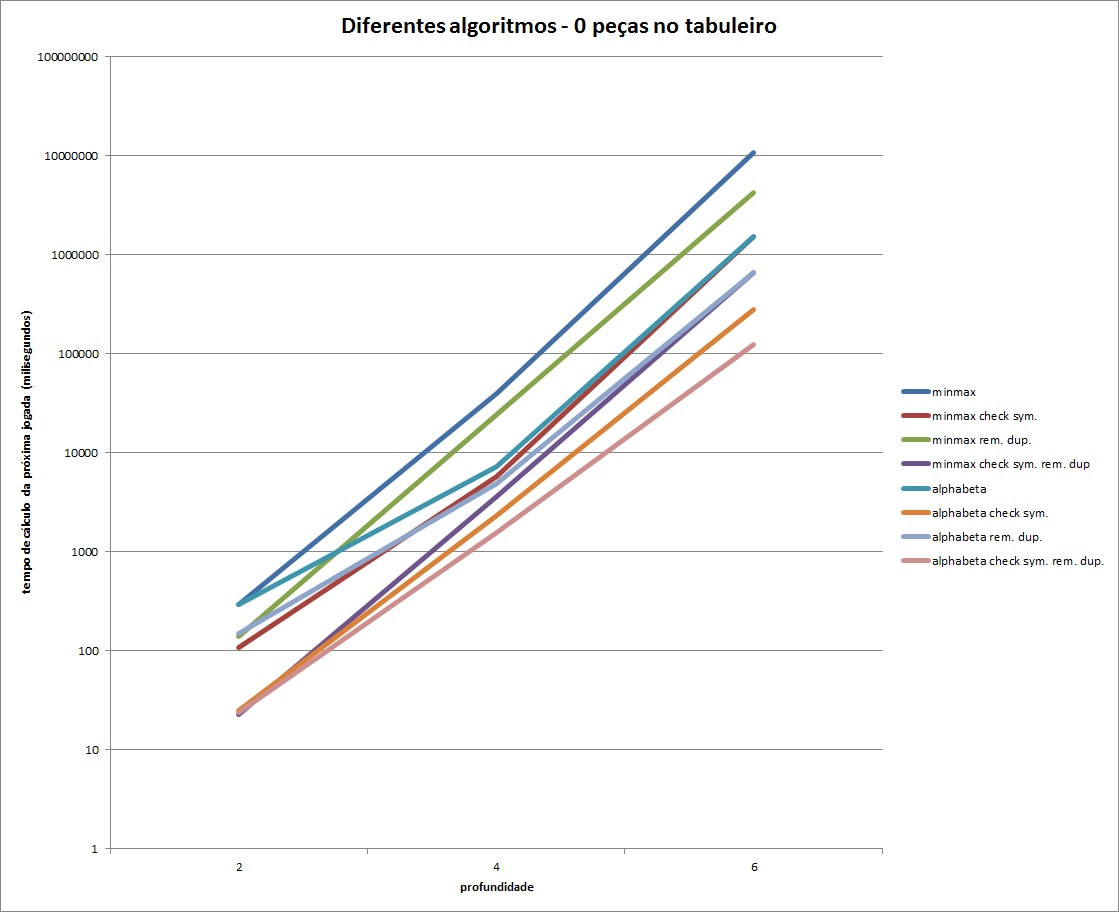
\includegraphics[height=11cm]{performance/tempP0depthComparison.jpg}
\end{table}

O gráfico tem escala logarítmica no eixo dos tempos, daí as retas aproximadas. Isto significa, como já era de esperar, que todos os algoritmos apresentam complexidade logarítmica. Também de esperar é a ordenação destes gráficos, sendo a melhor performance do alpha-beta com verificação de simetrias e remoção de duplicados e a pior do minmax sem qualquer melhoria.

\subsubsection{Variação do número de peças}

A variação do número de peças é útil para perceber que se pode obter resultados imediatos com níveis de profundidade diferentes ao longo do jogo. Enquanto que inicialmente o nível de profundidade 4 é o melhor que conseguimos, ao fim de 8 peças, já se consegue praticamente o mesmo tempo com nível de profundidade 6. Além disso, estes testes também ajudam a perceber quando é útil verificar as simetrias e remover duplicados.

\begin{table}[H]
\centering
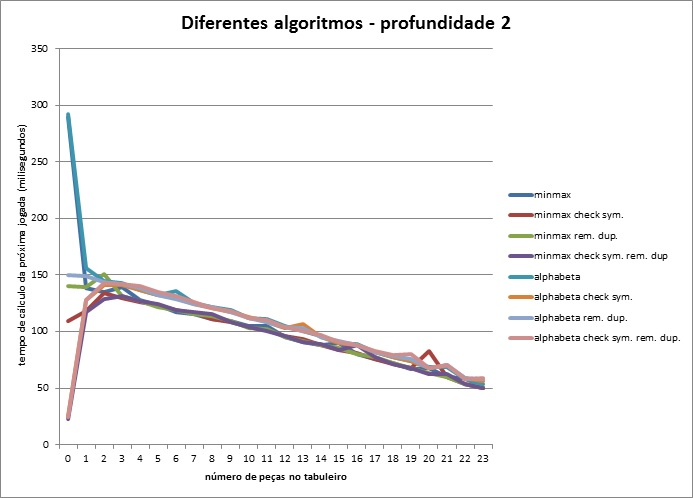
\includegraphics[height=12cm]{performance/tempPerfComparisonDepth2.jpg}
\end{table}

De reparar que a convergência total neste primeiro gráfico se deve ao facto de profundidade 2 corresponder apenas a uma jogada, não existindo por isso cortes alfa-beta.

\begin{table}[H]
\centering
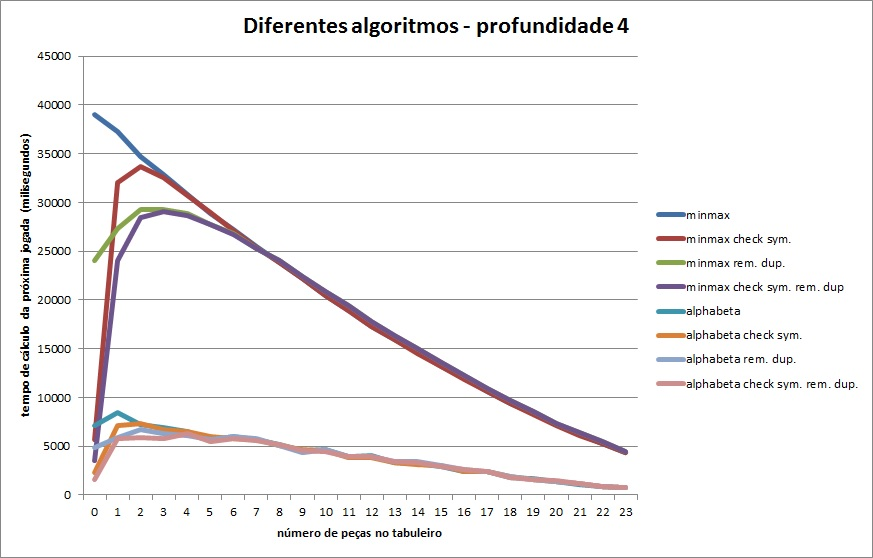
\includegraphics[height=10cm]{performance/tempPerfComparisonDepth4.jpg}
\end{table}

\begin{table}[H]
\centering
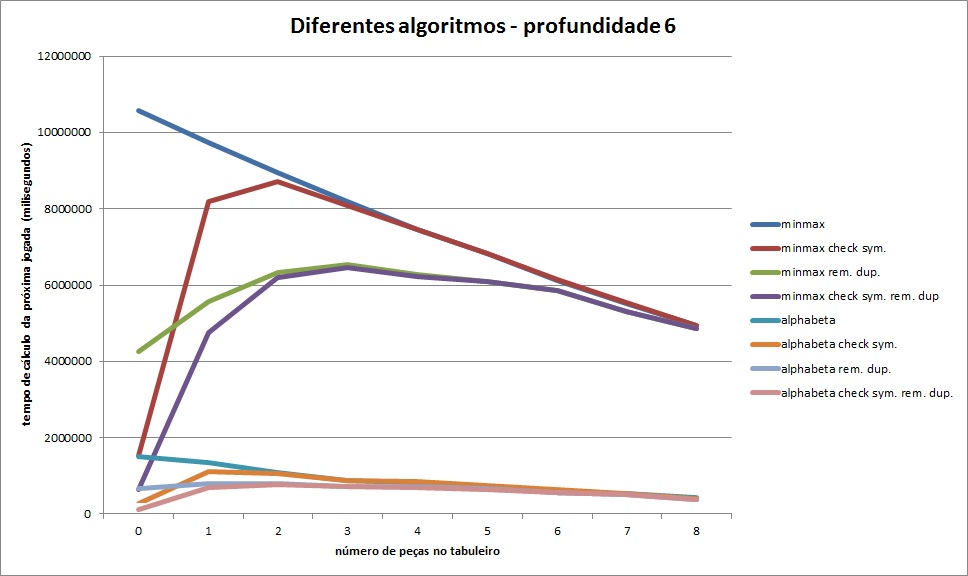
\includegraphics[height=9.5cm]{performance/tempPerfComparisonDepth6.jpg}
\end{table}



%---------------------------------------------------------------------%
%---------------------------------------------------------------------%
\newpage
%!TEX root=main.tex

\section{Conclusões}

Face às heurísticas implementadas, consideramos que o projeto se encontra sólido, sendo que a última implementada apresenta um comportamento bastante satisfatório contra jogadores humanos. 
%!TEX root=main.tex

\section{Futuras Melhorias}

Relativamente à componente de IA existem algoritmos e abordagens não exploradas. A implementação de ~\verb|iterative deepening|  em vez da realização de uma pesquisa única seria um ponto simples de implementar na continuação do projeto. A implementação de ~\verb|negaScout| e a ordenação de tabuleiros por uma ordem não aleatória baseada numa classificação de modo a facilitar a poda também seriam pontos interessantes a explorar.

Face à mini \verb|framework| implementada, seria interessante completá-la refinando e generalizando o PentagoPandora de modo a que consiga criar a árvore Minmax para qualquer jogo e para qualquer jogador.

O interface gráfico e a implementação em Unity3d pode ser ainda melhorada em diversos pontos, seja na apresentação, seja no código implementado. Com o intuito de disponibilizar parte do projeto na Asset Store do Unity3d, todo  grafismo presente não original deverá ser substituído e o código do projeto será revisto após a entrega do trabalho sendo que deverá ficar disponível para download antes de Outubro, caso passe nos testes de qualidade e não existam restrições legais que impeçam a publicação.







%---------------------------------------------------------------------%
%---------------------------------------------------------------------%
\newpage
\section{Recursos}

\subsection{Bibliografia}
\nocite{*}
\printbibliography[heading=none]

%!TEX root=main.tex

\subsection{Lista de Software e Serviços usados}

\begin{itemize}
\item \href{https://www.blender.org/}{Blender}
\item \href{https://eclipse.org/mars/}{Eclipse Mars} 
\item \href{https://github.com/}{Github}
\item \href{https://www.overleaf.com}{Overleaf}
\item \href{https://secure.logmein.com/home/pt}{Logmein}
\item \href{https://unity3d.com/pt}{Unity3d}
\item \href{https://www.visualstudio.com/}{Visual Studio}
\item \href{http://andrejv.github.io/wxmaxima/}{WxMáxima}
\end{itemize}
%!TEX root=main.tex

\subsection{Balanceamento da carga de trabalho}
\begin{itemize}
\item \^Angela Cardoso    %(30% ou mais. nao e debativel! |>__<|! ) 
\item Bruno Madeira \%  %(35% ou mais, nao e debativel! |>__<|! )
\item Francisco Veiga				
\end{itemize}

%=====================================================================
%=====================================================================
\newpage
\begin{appendices}

%!TEX root=main.tex


Para correr 

\newpage
\subsection{Code}
\subsubsection{IGameRules}
\label{IGameRules}

\begin{lstlisting}

/// <summary>
/// Interface that defines all the methods that must be implemented in order to use Minimaz Algorithm
/// </summary>
/// <typeparam name="GAME_BOARD">Class with the representation of the game's board</typeparam>
/// <typeparam name="GAME_MOVE_DESCRIPTION">Class with that is used to represent the game's player allowed moves/plays</typeparam>
public interface IGameRules<GAME_BOARD,GAME_MOVE_DESCRIPTION> { 
	
	GAME_MOVE_DESCRIPTION[] possible_plays(GAME_BOARD gb, int depth = 0);
	
	GAME_BOARD board_after_play(GAME_BOARD gb, GAME_MOVE_DESCRIPTION gmd);

	GAME_BOARD[] next_states(GAME_BOARD gb,int depth=0);

    /// <summary>
    /// checks if the game has ended.
    /// <para>returns null if game did not end or the value of utility if game ended</para>para>
    /// </summary>
    /// <param name="gb"></param>
    /// <param name="depth">optional usage, only usefull to calculate utility</param>
    /// <returns>null if game did not end or the value of utility if game ended</returns>
    float? game_over(GAME_BOARD gb,int depth);

    /// <summary>
    /// method to be used when minimax achieves max depth
    /// <para>may have a heuristics 'selector' in the implementation </para>
    /// <para>may return Float.POSITIVE_INFINITY or Float.NEGATIVE_INFINITY to force prioritization of certain plays</para>
    /// </summary>
    /// <param name="gb"></param>
    /// <returns></returns>
    float evaluate(GAME_BOARD gb);

    /// <summary>
    /// Should select the next node type to use in minimax. 
    /// <para>Default behaviour for most games should be return !currentIterationNode.</para>
    /// <para>Some Games, like pentago, need some additional considerations due to 'half step/play' endgames</para>
    /// </summary>
    /// <param name="gb"></param>
    /// <param name="currentIterationNode"></param>
    /// <returns></returns>
    bool selectMINMAX(GAME_BOARD thisnode_gb, bool currentIterationNode);

    /// <summary>
    /// decide what depth to use on minimax depending on the game board
    /// </summary>
    /// <param name="gb"></param>
    /// <returns></returns>
    int smart_depth(GAME_BOARD gb);

    /// <summary>
    /// get information about 'Rules' to print/display
    /// </summary>
    /// <param name=""></param>
    /// <returns></returns>
    string toDisplayString();
}

\end{lstlisting}
\end{appendices}

\end{document}